A lo largo de los capítulos anteriores se han repasado los conceptos fundamentales que atañen 
al proceso de contratación pública electrónica, la casuística, beneficios y métodos disponibles 
para la aplicación de los principios de \opendata, \linkeddata y Web Semántica a distintos dominios 
de conocimiento. Por otra parte, se ha realizado una definición de un ciclo de vida de datos enlazados 
describiendo procesos, métodos y tareas cuya aplicación conlleva una promoción sostenible de datos a las iniciativas 
previamente citadas, tal y como se ha señalado en el Capítulo~\ref{capitulo:metodos-separados}. Finalmente, con el objetivo 
de suministrar soporte a este ciclo de vida se han implementado una serie de componentes desde un punto de vista de la 
ingeniería. La siguiente etapa, por tanto, corresponde a la validación del trabajo realizado mediante experimentos en los 
cuales se pueda cuantificar el enfoque realizado, en este sentido, la experimentación posible es muy variada, pero atendiendo 
a la hipótesis de partida y a los componentes implementados es posible identificar los siguientes experimentos:

\begin{enumerate}
 \item Experimento para la validación de los datos transformados desde un punto de vista cuantitativo y cualitativo, comparando las versiones 
actuales de los datos disponibles con la versión generada tras la aplicación de los métodos semánticos a las entidades 
implicadas en los anuncios de licitación de un proceso de contratación pública.
\item Experimento para la verificación de la construcción de un sistema de recuperación de información utilizando una fuente 
de datos basada en \linkeddata y tecnologías semánticas.
\item Experimento para la evaluación del rendimiento del sistema construido desde un punto de vista cuantitativo.

\end{enumerate}

El diseño de estos experimentos permite por una parte, la verificación de la hipótesis objeto de estudio en este trabajo y, por otra parte, 
la validación de la construcción de sistemas basados en \linkeddata y tecnologías semánticas.

\subsection{Consideraciones Generales}\label{exp-general}
Es preciso señalar que todos los experimentos llevados a cabo se realizan 
bajo la ejecución de un plan detallado, las etapas a seguir serán las siguientes:

\begin{enumerate}
 \item Definición de los objetivos del experimento. 
\item Selección de una regla de asignación de las unidades experimentales a las condiciones de estudio. 
\begin{itemize}
 \item Cualitativos: tipo de entorno hardware y software, etc. En este caso, se pueden fijar las condiciones \textit{hardware} y \textit{software}:
  \begin{itemize}
  \item Servidor. El software consta de un repositorio \gls{RDF} Virtuoso de OpenLink (version 06.01.3127) desplegado sobre una máquina 
  virtual de Virtual Box (version 4.0.6) sobre un sistema operativo Linux 2.6.35-22-server \#33-Ubuntu 2 SMP x86\_64 GNU/Linux Ubuntu 10.10 con 2GB de RAM y 30GB HardDisk, la 
  máquina física utilizada como anfitrión es un PC DELL con la misma configuración software que la máquina virtual.
  \item Cliente. En este caso el cliente es un Notebook DELL XPS M1330 con un sistema operativo Linux 2.6.32-24-generic \#43-Ubuntu SMP x86\_64 GNU/Linux con 4GB de RAM, las distintas 
  réplicas son ejecutadas a través de la herramienta Java, Junit.
  \end{itemize}
 \item Cuantitativos: tamaño de la muestra, de la memoria y número de posibilidades de expresar una consulta.
\end{itemize}
 \item Especificación de las medidas de trabajo en cuanto a la respuesta.
 \item Ejecución de un experimento piloto. 
 \item Especificación de un modelo.
 \item Esquematización de los pasos a seguir. 
 \item Determinación del tamaño muestral.
 \item Revisión de las decisiones anteriores.
\end{enumerate}


\section{Experimento sobre la aplicación de \textit{Linked Data} a las Licitaciones Públicas}
\subsection{Diseño del experimento sobre la aplicación de \textit{Linked Data} a las Licitaciones Públicas}
Con el objeto de la validación de la hipótesis de partida surge la necesidad de comprobar si el ciclo de vida 
utilizado para la promoción de los datos concernientes a los anuncios de licitación y sus derivados como las 
clasificaciones de productos y las organizaciones ha sido convenientemente ejecutado. Las ventajas 
de uso de \linkeddata, \opendata y la aplicación de tecnologías semánticas ha sido convenientemente 
revisada en la Sección~\ref{capitulo:semantica}, por lo que aplicando los principios promulgados bajo 
esta iniciativa y realizando la correspondiente evaluación de los mismos con resultados positivos 
se estima, evidentemente, que las ventajas adicionales se obtienen de forma automática. Por ejemplo, 
en el caso de suministrar los datos bajo los protocolos y estándares actuales de Internet se asegura 
la interoperabilidad y facilidad de acceso, con lo que utilizando \gls{HTTP URI}s este principio y sus correspondientes 
ventajas quedarían perfectamente demostradas.

Por otra parte, cabe mencionar que la evaluación de los datos ha sido abordada bajo distintos paradigmas, 
como la calidad. En este contexto existen muchos trabajo que tratan de definir métricas sobre cómo determinar
si unos datos son lo suficientemente ``buenos'' pero tanto en las tradicionales bases de datos como en el emergente 
paradigma de datos enlazados, las herramientas, vocabularios y especificaciones para establecer la calidad de los datos 
se centran en evaluar el cumplimiento de ciertas características definidas por los autores pero que en ningún caso 
son de obligado cumplimiento, más bien se trata de buenas prácticas. En este sentido, el enfoque seguido en este experimento 
se basa en la recopilación de buenas prácticas, patrones de diseño, condiciones de los conjuntos de datos para pertenecer 
a una determinada iniciativa, experiencia adquirida, etc., en las cuales se fijan los criterios que posteriormente pueden 
ser expresadas en los vocabularios y herramientas disponibles para obtener los valores que estas tecnologías suministran. En este sentido, 
se dispone de herramientas como \gls{WIQA}~\cite{bizer2007,citeulike:3875270} o LINK-QA~\cite{link-qa} que ofrecen de un lenguaje de patrones para valorar la pertenencia de una tripleta 
a un determinado grafo, por ejemplo evaluando si una propiedad tiene un determinado valor. Por otro lado, se ha propuesto el vocabulario 
\gls{LODQ}~\cite{lodq} para la creación de métricas enclavadas en una ordenación mayor pero cuya implantación se encuentra en una etapa muy temprana. Es necesario 
destacar que en su mayor parte los criterios de evaluación requieren una validación semi-manual por lo que el empleo de herramientas 
aunque es conveniente debe ser valorado para no incurrir en un exceso mayor que la propia validación. En el caso objeto de estudio, 
el enfoque seguido se centra en el cumplimiento de criterios para pertenecer a las iniciativas \linkeddata, \opendata y la suma 
de ambas. En cuanto a la corrección en los valores de los datos se supone, en parte, asumida ya que todos los datos 
proceden de fuentes oficiales y en el caso concreto de los anuncios de licitación han sido previamente validados 
por la empresa Gateway S.C.S. No obstante, hay que destacar que la calidad de datos en \linkeddata es una línea 
de investigación interesante y emergente en la cual se está empezando a avanzar pero que no se ha declarado estratégica en estos primeros años, 
a la vista del número de trabajos existentes hasta la fecha.

En el caso objeto de estudio, el punto de partida son conjuntos de datos generados por las Administraciones Públicas y ya procesados por una empresa por lo que parcialmente la fuente de los mismos se considera 
fiable en cuanto a requerimientos de calidad, adicionalmente y debido a la aplicación de un proceso de transformación de datos utilizando 
herramientas apropiadas para ello y mediante la consecución de tareas determinadas permite asegurar, en un alto grado, el mantenimiento 
de la calidad, minimizando los posibles errores de transformación. Finalmente la evaluación a través de las tablas de validación permite asegurar que los datos generados 
cumplen criterios de accesibilidad, calidad, etc., igualmente éstos se pueden expresar en las herramientas y vocabularios 
citados, en su gran mayoría, por lo que en último término la aportación de los mismos es simplemente la validación automática y la extracción de métricas 
o estadísticas de uso basadas en criterios de clusterización, etc., fijados por las propias herramientas. 

El diseño de este experimento, por tanto, se planifica desde dos puntos de vista:
\begin{description}
 \item [Cuantitativo.] La pregunta principal planteada en este caso se refiere a si con el uso de datos enlazados es posible 
facilitar el acceso a un mayor número de recursos relacionados con los anuncios de licitación y, en consecuencia, a la información 
y datos disponibles en los mismos.
\item [Cualitativo.] La cuestión planteada en este caso se centra en valorar si el proceso de generación y transformación de datos 
a la iniciativa de datos enlazados se puede valorar respecto a una serie de criterios y buenas prácticas.
\end{description}

Adicionalmente la evaluación debe asegurar que se cumplen los principios básicos de \linkeddata y \opendata con lo que 
se aseguran los beneficios y ventajas promulgados por estas iniciativas.

\subsubsection{Punto de vista Cuantitativo}
Una vez presentados las directrices básicas del experimento es necesario realizar la exposición del plan detallado 
y diseño del mismo. Para el primer caso, la evaluación cuantitativa debe suministrar la prueba de que el uso de datos 
enlazados permite facilitar el acceso a un mayor número de anuncios de licitación en general, y a una mayor cantidad de datos 
e información relativa al proceso de licitación pública electrónica en particular. Con ello, se demuestra que el uso de este 
enfoque favorece una mayor expresividad en la consulta de información y los datos. Las etapas a seguir serán las siguientes:

\begin{enumerate}
 \item Definición de los objetivos del experimento. Las preguntas a responder por el experimento serán:
\begin{itemize}
 \item ¿Cuál es la expresividad actual, en términos de número de conceptos para realizar consultas, para el acceso a la información de anuncios de licitación?
 \item ¿Cuál es la ventaja de uso de un modelo \gls{RDF} para la expresión y recuperación de la información de los anuncios de licitación?
 \item ¿Cómo los datos enlazados favorecen el aumento de expresividad en la ejecución de consultas y por tanto facilitan la recuperación de los 
anuncios de licitación? 
 \item ¿Cuál es el beneficio real del uso de datos enlazados para representar la información? 
 \item ¿Se incurre en algún error al aumentar la expresividad?
\end{itemize}

\item Selección de una regla de asignación de las unidades experimentales a las condiciones de estudio. En este caso, 
la unidad experimental de este estudio será un repositorio RDF en el cual se encuentra albergada la información 
sobre los anuncios de licitación, las clasificaciones de productos y las organizaciones.
\begin{itemize}
 \item Cualitativos: tipo de entorno hardware y software, expresividad de las consultas.
 \item Cuantitativos: tamaño de la muestra, de la memoria y número de posibilidades de expresar una consulta.
\end{itemize}

En cuanto a la caracterización de los factores cualitativos, respecto al entorno hardware y 
software se utiliza el definido en la Sección~\ref{exp-general}. 

Sobre la expresividad de las consultas cabe mencionar que no es de recibo establecer una comparación entre un sistema de búsqueda sintáctico 
tradicional basado en texto libre con uno basado en un vocabulario controlado ya sea mediante la concatenación de filtros u otro tipo 
de acotación de la búsqueda. Es por ello que como referente para realizar la comparación tomaremos un sistema de búsqueda que permite 
seleccionar los códigos \gls{CPV} 2008 sobre los cuales realizar búsquedas de anuncios de licitación, la justificación de esta decisión reside 
en que la mayoría de los actuales sistemas de búsqueda huyen del texto libre (obviamente los resultados son menos ajustados) y sólo 
permiten la introducción de varios códigos CPV para la recuperación de documentos. Este es el caso de la herramienta Euroalert.net de Gateway S.C.S. 
o de otros sistemas como Licitaciones.es, etc., igualmente en el ámbito de los datos enlazados, la propuesta realizada en el proyecto LOTED 
se basa en la introducción de códigos para generar consultas en \gls{SPARQL}. Dada esta situación, la comparación se realizará entre una versión 
básica que acepta el CPV 2008 como vocabulario controlado, $10357$ términos, de búsqueda sobre los datos que se han transformado en la Capítulo~\ref{capitulo:metodos-separados}, 
$1M$ de anuncios de licitación y $50000$ organizaciones.

 \item Especificación de las medidas de trabajo en cuanto a la respuesta. En este caso la medida utilizada para valorar los resultados y 
será en magnitud del número de nuevos términos/conceptos que se pueden utilizar al añadir un nuevo vocabulario controlado en el campo 
de las clasificaciones de productos y enlazarlo con el \gls{CPV} 2008.
 \item Ejecución de un experimento piloto. Con el objetivo de ejemplificar el modelo y diseño del experimento se realiza un 
ejemplo a pequeña escala para facilitar la compresión del mismo y realizar una validación previa del enfoque seguido.
 \item Especificación de un modelo. En este sentido, la consecución del experimento permite establecer una fórmula sencilla 
para la predicción de la ganancia expresiva al añadir un nuevo vocabulario de negocio y enlazarlo con el CPV 2008 y \textit{ProductOntology}. De 
esta forma, se suministra un valor a la ganancia expresiva del uso de datos enlazados en este dominio.
 \item Esquematización de los pasos a seguir. Las etapas a cumplir por este experimento, una vez que las clasificaciones de productos 
se encuentran transformadas reside en la extracción de consultas en \gls{SPARQL} para establecer el número de enlaces entre las mismas y 
la realización de un \texttt{script} para la generación de datos finales. Específicamente se realizan los siguientes pasos:
\begin{enumerate}
 \item Estado inicial: clasificaciones de productos ya transformadas y disponibles a través de un \textit{endpoint} de SPARQL.
 \item Extracción de los términos de una \gls{PSC} relacionados con el CPV 2008. Para ello se puede realizar las siguientes consultas 
en SPARQL, ver Figura~\ref{fig:step-1}, generando dos ficheros: \texttt{psc-1} y \texttt{psc-2} con los resultados de la consultas respectivamente.

\begin{figure}[!htp]
\begin{lstlisting}
SELECT DISTINCT ?psck WHERE {
  ?psck rdf:type pscs:PSCConcept.
  ?psck skos:inScheme <http://purl.org/weso/pscs/sitc/v4/resource/ds> .
  ?psck skos:closeMatch ?cpvk.
}

SELECT DISTINCT ?psck WHERE {
  ...
  ?psck skos:exactMatch ?cpvk.
}
\end{lstlisting}
	\caption{Consultas en SPARQL de extracción de términos de una PSC relacionados el CPV 2008.}
	\label{fig:step-1}
\end{figure}

\item Extracción de los términos una PSC, incluida el CPV 2008, relacionados con \textit{ProductOntology} y de los términos en \textit{ProductOntology} 
respecto a una PSC, generando dos ficheros: \texttt{psc-5} y \texttt{cpv-2008-6}.

\begin{figure}[!htp]
\begin{lstlisting}
SELECT DISTINCT ?psck WHERE {
  ...
  ?psck pscs:relatedMatch ?pok.
}

SELECT DISTINCT ?pok WHERE {
  ...
  ?psck pscs:relatedMatch ?pok.
}
\end{lstlisting}
	\caption{Consultas en SPARQL de extracción de términos de una PSC con \textit{ProductOntology}.}
	\label{fig:step-1}
\end{figure}

\item Generación del fichero obtenido de las consultas realizadas en el Paso 2 con los enlaces reales 
de una PSC al CPV 2008. La extracción del número de enlaces se realiza mediante el comando: 
\texttt{cat psc-1 psc-2 | sort | uniq | wc -l}

\item Generación del fichero intersección con los elementos de \textit{ProductOntology} provenientes 
de una PSC y el CPV 2008. La intersección se realiza mediante el comando: \texttt{awk 'NR==FNR{a[\$0];next} \$0 in a' psc-5 cpv-2008-6  > psc-5-6}

\item Generación del listado final de términos únicos de una PSC que tienen enlace directo con el CPV 2008 
o bien a través de \textit{ProductOntology}. Para la realización de esta operación se ha implementado 
un sencillo programa en Java que toma el fichero anterior, \texttt{psc-5-6}, el fichero RDF con los 
datos de la PSC y genera un listado de conceptos pertenecientes a la PSC, fichero \texttt{psc-po-cpv}, que tienen una relación 
con un elemento de \textit{ProductOntology} presente en el fichero de entrada.

\item Extracción del número final de elementos que realmente se encuentran enlazados entre la PSC y el CPV 2008, 
directamente o bien a través de \textit{ProductOntology}, esta operación se realiza mediante el comando:
\texttt{cat psc-1 psc-2 psc-po-cpv | sort | uniq | wc -l }

\item Adición de todos los valores recogidos para la creación de porcentajes mediante un hoja de cálculo.
\end{enumerate}

 \item Determinación del tamaño muestral. Ya se han señalado en los aspectos cuantitativos del experimento
 \item Revisión de las decisiones anteriores.
\end{enumerate}

\subsubsection{Punto de vista Cualitativo}
De acuerdo a la introducción realizado, el objetivo de este experimento se centra en la evaluación y grado 
de cumplimiento de buenas prácticas sobre el uso de datos enlazados, principios de \linkeddata y \opendata, 
patrones de diseño y características para la adición de \datasets \gls{RDF} a la nube de datos enlazados abiertos 
y a registros tipo \gls{CKAN}. Esta evaluación permite discernir qué enfoques cumplen estos requisitos y principios 
para así determinar en qué grado se encuentran unos datos respecto a las iniciativas ya mencionadas. Este 
enfoque permite establecer si el ciclo de vida de generación de datos ha asegurado la calidad de los mismos 
en cuanto a grado de cumplimiento de criterios. A continuación se detalla el plan de experimentación en los 
siguientes pasos:

\begin{enumerate}
 \item Definición de los objetivos del experimento. Las preguntas a responder por el experimento serán:
\begin{itemize}
 \item ¿El ciclo de vida seguido y los datos generados certifican la aplicación de buenas prácticas de \linkeddata?
 \item ¿El ciclo de vida seguido y los datos generados certifican el cumplimiento de los principios de \linkeddata?
 \item ¿Qué nivel del modelo de 5 $\star$ se puede establecer?
 \item ¿Qué porcentaje de patrones de diseño se han aplicado en los datos generados?
 \item ¿Los datos generados pueden pertenecer a la nube de datos enlazados abiertos?
 \item ¿Los datos generados pueden pertenecer a un registro CKAN? 
 \item ¿El ciclo de vida seguido y los datos generados certifican el cumplimiento de los principios de \opendata?
 \item ¿Se puede asegurar que los datos son enlazados y abiertos?
 \item ¿Qué beneficios se obtienen del cumplimiento de estos objetivos?
\end{itemize}

\item Selección de una regla de asignación de las unidades experimentales a las condiciones de estudio. En este caso, 
la unidad experimental de este estudio será cada uno de los \dataset \gls{RDF} generados para los anuncios de licitación públicos, 
el catálogo de clasificaciones de productos y las organizaciones.
\begin{itemize}
 \item Cualitativos: tipo de entorno hardware y software, grado de cumplimiento de los criterios.
 \item Cuantitativos: tamaño de la muestra, número de criterios en cada una de las tablas de validación, selección 
de enfoques a comparar.
\end{itemize}

En cuanto a la caracterización de los factores cualitativos, respecto al entorno hardware y 
software se utiliza el definido en la Sección~\ref{exp-general}. 

Sobre el grado de cumplimiento de criterios se establece un valor numérico y un porcentaje del grado de cumplimiento 
para cada una de las tablas de criterios creadas y para cada uno de los enfoques evaluados. De esta forma, se da respuesta 
a las preguntas planteadas al punto anterior especificando en que nivel de cumplimiento se encuentra cada uno de los 
enfoques.

Respecto a los aspectos cuantitativos, el desarrollo del experimento consiste en la evaluación de $196$ criterios, como una 
encuesta sobre los enfoques seleccionados, distribuidos en distintas tablas que permitan establecer correctamente los 
aspectos cualitativos. El diseño de estas tablas se presenta en el Apéndice~\ref{tablas-validacion-apen} con las preguntas 
y la respuesta ideal de cada una de ellas. Con este enfoque se permite realizar un repaso pormenorizado de los criterios 
y realizar así una evaluación intensiva. Aunque algunos de los enfoques pertenecen a distintas disciplinas y han sido 
realizados con distintos objetivos a los presentes en la iniciativa de datos enlazados, si es posible establecer 
ciertas características en común por lo que la comparación es posible si nos remitimos al acceso a la información 
y a los datos. Por tanto, en cuanto a los enfoques seleccionados, se comparan los más representativos 
para cada uno de los \datasets RDF, de esta forma se han seleccionado los siguientes:
\begin{enumerate}
 \item Anuncios de licitación públicos, teniendo en cuenta que la publicación de estos anuncios es transversal 
desde la Unión Europea hasta organismos de carácter local publicando en los correspondientes boletines oficiales se han 
agrupado y escogido los siguientes:
\begin{itemize}
 \item Boletines y Publicaciones oficiales: \gls{TED} y \gls{BOE}. El objetivo es aunar la forma en la que los boletines 
oficiales publican la información y los datos de licitación. Se han seleccionado estas dos fuentes porque 
son oficiales y porque representan gran parte de la casuística: 1) información restringida con un modelo formal (\gls{XML Schema}) pero con necesidad 
de suscripción (TED) y 2) información total pero en peores condiciones de publicación (BOE). Teniendo en cuenta 
que el comportamiento de los boletines oficiales es similar, la selección de uno de ellos se considera representativa, además, 
en los últimos años el BOE ha avanzado enormemente en la provisión de servicios de búsqueda, uso de capacidades avanzadas 
de \gls{PDF} y mejora de la generación de \gls{HTML}, por lo que dispone de un conjunto de características verdaderamente interesantes 
en términos de evaluación.
 \item Plataformas de contratación: Plataforma de Contratación del Estado. Este enfoque supone un avance a la simple 
publicación en boletines oficiales ya que los datos y la información están disponibles bajo un modelo formal (XML Schema) pero 
ocurre en cierta manera lo mismo que en TED, es necesaria una suscripción para el acceso completo. No obstante, teniendo 
en cuenta la proliferación de este tipo de plataformas, tanto públicas como privadas (por ejemplo \gls{opXML} del proyecto ``10ders Information Services'') 
es necesario y conveniente incluirlas dentro del proceso de comparación.
 \item Servicios de terceros que reutilizan la información oficial, se han agrupado los suministrados por 
Euroalert.net y Licitaciones.es. La característica de estos servicios es similar, permiten la búsqueda y acceso 
a las licitaciones de forma restringida, a partir de este punto, para realizar la consulta de datos e información 
de forma completa se debe disponer de una suscripción. En general, no es posible conocer el modelo de datos utilizado 
ni la tecnología subyacente pero desde el punto de vista del acceso a la información son muy relevantes ya que 
suponen servicios de negocio.
\item LOTED. Se trata del primer gran esfuerzo por aunar tecnología semántica y datos enlazados reutilizando la información 
abierta publicada en TED a través de los \gls{RSS}. En cuanto a comparación, sin duda este enfoque es un buen reflejo para el realizado 
con MOLDEAS.
\end{itemize}


\item Clasificaciones de Productos, en este caso las posibilidades están restringidas a las publicaciones oficiales 
en formato \gls{CSV} o MSExcel por lo que será el único caso en común para todas las clasificaciones. No obstante, en cuanto 
al CPV y otras clasificaciones tipo NAICS, existen servicios de consulta \textit{on-line} en forma de sistemas de búsqueda o directorios para navegar 
por la jerarquía.

\item Organizaciones, como subconjunto de la información proveniente de los anuncios de licitación públicos se utilizan 
fuentes similares de información, entre las cuales se encuentran:
\begin{itemize}
 \item Boletines y Publicaciones oficiales: \gls{TED} y \gls{BORME}.
 \item Plataforma de Contratación del Estado.
 \item Servicios de terceros.
 \item Bases de datos administrados por terceros, en este caso, existen algunas empresas que comercializan 
una base de datos con información corporativa pero sin publicar la información y los datos vía web. Este es 
el caso de la Cámara de Comercio.
 \item \textit{OpenCorporates}, por analogía con LOTED, se trata del primer gran esfuerzo por promocionar 
la información corporativa mediante la aplicación de los principios de \opendata y \linkeddata, convirtiéndose 
en un enfoque pionero y de referencia a nivel mundial.
\end{itemize}
\end{enumerate}


 \item Especificación de las medidas de trabajo en cuanto a la respuesta. En este experimento específico los valores 
para cada uno de los criterios evaluados podrán ser de los siguientes tipos:
\begin{enumerate}
 \item Valor positivo, \si, si es un criterio que debe tener y se cumple.
 \item Valor negativo, \no, si es un criterio que debe tener y no se cumple.
 \item Valor no aplicable, \na, si es un criterio que se desconoce, que se solapa con otro (por ejemplo 
en la tabla de cumplimiento del registro \gls{CKAN} o bien los datos son \textit{published-by-producer} o 
por \textit{published-by-third-party}) o no está asociado a ese enfoque.
\end{enumerate}

La suma de todas las valoraciones permite establecer un grado de cumplimiento. Adicionalmente, las tablas de 
validación se han diseñado para que aporten la mayor información posible agrupando los criterios similares. Es conveniente 
destacar que el número de valores no aplicables nunca debe ser menor que el propuesto en el modelo de referencia.

 \item Ejecución de un experimento piloto. Con el objetivo de probar el diseño de las tablas de validación 
se ha realizado un experimento inicial en el cual se ha detectado: 1) que algunos criterios no estaban 
correctamente divididos y no permitían discernir ciertos factores, por ejemplo inicialmente los principios 
de \linkeddata y los criterios del modelo 5 $\star$ estaban juntos y se ha decidido separarlos para facilitar 
la evaluación posterior. Igualmente, los principios de \opendata estaban unidos a los beneficios y ventajas de este enfoque, por lo que también 
se han separado en dos tablas. En resumen, de la versión inicial se han generado dos tablas nuevas. 2) Se han incluido nuevos criterios respecto a la versión inicial para incluir características de metadatos 
en la evaluación como es el sellado en el tiempo de los datos y la información. En este caso, el experimento piloto ha servido para detectar un diseño incorrecto de la encuesta e incluir nuevos 
criterios.

 \item Especificación de un modelo. En este caso se establece un modelo de respuestas ideal como referencia, a partir del 
cual se puede evaluar el grado de cumplimiento. No obstante, la combinación de las distintas valoraciones es conveniente 
realizarla por separado y no mezclar las distintas encuestas con el objetivo de no introducir ruido y falsos positivos 
en los resultados.

 \item Esquematización de los pasos a seguir. Las etapas a cumplir para la realización de los cuestionarios por cada 
uno de los enfoques seleccionados es el siguiente:
\begin{enumerate}
 \item Establecimiento del modelo de referencia, con los valores admitidos.
 \item Revisión uno a uno de los criterios, consultando cada una de las fuentes de información y datos para 
cada enfoque.
 \item Agregación de los resultados y valoraciones.
 \item Extracción de estadísticas, contraste de hipótesis, validación y evaluación.
\end{enumerate}

\end{enumerate}

\subsection{Ejecución del experimento sobre la aplicación de \textit{Linked Data} a las Licitaciones Públicas}

\subsubsection{Punto de vista Cuantitativo}
La ejecución de este experimento requiere la expresión formal de los datos para establecer desde un punto 
de vista cuantitativo el porcentaje de ganancia en expresividad pasando de utilizar un vocabulario controlado para la realización 
de consultas a una serie de los mismos mediante datos enlazados. En este caso, la recuperación de información 
entre la búsqueda habitual (texto libre) y un vocabulario controlado difiere en que el universo del discurso es 
en el primer caso infinito y en el segundo finito, determinado por el número de términos del vocabulario. En los anuncios 
de licitación se parte de las siguientes premisas:
\begin{itemize}
 \item Todo anuncio de licitación está etiquetado al menos con un código/término perteneciente al \gls{CPV} 2008.
 \item El uso de los códigos CPV es obligatorio en todos los anuncios de licitación a nivel europeo, como 
se ha señalado en la Sección~\ref{sect:pscs}.
 \item La única información obligatoria, además del emisor del anuncio de licitación, son los códigos CPV 2008.
\end{itemize}

Bajo estas circunstancias la muestra sobre la que se realiza el experimento cuenta con las siguientes características:
\begin{itemize}
 \item Se cuenta con una base documental $\mathcal{D}$ constituida por $1$ millón de anuncios de licitación.
 \item La clasificación de productos (vocabulario controlado $\mathcal{V}$ para contrato públicos) 
del CPV 2008 está formado $\#\mathcal{V} = 10357$ códigos/términos distintos.
 \item Cada uno de los documentos $d \in \mathcal{D}$ está etiquetado con al menos un código $v \in \mathcal{V}$.
\end{itemize}

Una vez caracterizado el entorno de pruebas, cabe formular cómo se calcula la ganancia de añadir un nuevo vocabulario 
mediante \linkeddata.
\begin{itemize}
 \item El nuevo vocabulario controlado $\mathcal{V}_{psc}$ dispone $\#\mathcal{V}_{psc}$ términos.
 \item El enlazado de datos genera de este vocabulario respecto a uno objetivo $\mathcal{V}$ presenta los siguientes
casos:
\begin{enumerate}
 \item Enlace 1-1, es decir, existen términos $v^k_{psc} \in \mathcal{V}_{psc}$ que se enlazan con un sólo término $v^k \in \mathcal{V}$ 
generando $K$ enlaces.
 \item Enlace 1-n, es decir, existen términos $v^k_{psc} \in \mathcal{V}_{psc}$ que se enlazan con varios términos $v^k \in \mathcal{V}$ 
generando $K_n$ enlaces.
\end{enumerate}
\item El resultado de esta operación es un conjunto de pares de enlaces $\{ (v^0_{psc},v^0), (v^k_{psc},v^k)..(v^n_{psc},v^n) \}$.
\item Dada esta situación el vocabulario inicial $\mathcal{V}$ ha sido incrementado en todos los elementos $v^k_{psc} \in \mathcal{V}_{psc}$  
para los cuales existe un enlace con algún elemento $v^k \in \mathcal{V}$ .
\item El número de nuevos términos en los que el vocabulario $\mathcal{V}$ es incrementado es igual al conjunto 
de elementos $v^k_{psc}$, denominado  $\mathcal{V'}_{psc}$, con algún enlace a $\mathcal{V}$ (estrictamente sin repeticiones por definición de conjunto).
\item El porcentaje de ganancia de expresividad, en el sentido de cuántos nuevos términos permiten pasar de $\mathcal{V}_{psc}$ a 
$\mathcal{V}$, es el siguiente:

\begin{definition}{Porcentaje de Ganancia}
\begin{align}
\% =  \langle (\#\mathcal{V'}_{psc}+\#\mathcal{V}) / \#\mathcal{V} \rangle * 100 - 100
\end{align}
\end{definition}

\item Finalmente, y en el caso concreto de las clasificaciones de productos/taxonomías, existe la posibilidad de que elementos 
$v^j_{psc} \in \mathcal{V}_{psc}$ no estén directamente relacionados con el conjunto $\mathcal{V}$ pero de acuerdo a la jerarquía 
de términos en $\mathcal{V}_{psc}$ se pueda pensar que si $v^j_{psc}$ está relacionado con $v^k_{psc}$ a través de una relación $r_k$, 
entonces $v^j_{psc} \in \mathcal{V'}_{psc}$. Este tipo de enfoque es crítico debido a que provoca una situación recursiva e infinita, 
uno de los problemas actuales de \linkeddata a la hora de realizar consultas, pero debido a que el vocabulario $\mathcal{V}_{psc}$ es 
finito y las relaciones entre sus términos es de jerarquía, se puede establecer un valor máximo para el porcentaje de 
ganancia que ocurrirá cuando $\mathcal{V}_{psc} \equiv \mathcal{V'}_{psc}$.

\end{itemize}

Como ejemplo para la validación de este enfoque se utilizarán los siguientes conjuntos:
\begin{itemize}
 \item Sea $\mathcal{V} = \{ 1, 2, 3 \}$  y  $\mathcal{V}_{psc} = \{A, B, C, D, E\}$.
 \item El conjunto de pares enlaces es el siguiente: $\{ (A,1), (B,2), (C,1) (C,2) \}$.
 \item Por tanto, el conjunto $\mathcal{V'}_{psc} = \{A, B, C\}$ y el porcentaje de ganancia en expresividad será el siguiente:

\begin{align}
\% =  \langle (3+3) / 3 \rangle * 100 = 200 - 100 = 100 
\end{align}
\item Lo que implica que el número de términos final es el doble que el inicial, aumentando así la expresividad en un $100\%$.
\end{itemize}


Adicionalmente e introduciendo un nivel más de indirección mediante de las \gls{PSC}s con \textit{ProductOntology} se da el siguiente caso:
\begin{itemize}
 \item Existe un conjunto $\mathcal{V''}_{psc}$ que representa la unión de todos los $\mathcal{V'}_{psc}$ correspondientes 
a los enlaces entre una determinada PSC y \textit{ProductOntology}, estrictamente conteniendo el elemento de \textit{ProductOntology} de cada par.
\item Existe un conjunto $\mathcal{V'}_{cpv}$ que representa el conjunto de pares de enlaces entre el \gls{CPV} 2008 y \textit{ProductOntology}, 
estrictamente conteniendo el elemento de \textit{ProductOntology} de cada par.
\item La intersección entre $\mathcal{V''}_{psc} \sqcap \mathcal{V'}_{cpv}$ representa el conjunto de todos enlaces mediante 
los cuales se puede realizar el salto entre una PSC al CPV 2008 a través de \textit{ProductOntology}. Los elementos 
de cada PSC que permitan acceder al CPV 2008 de esta forma y no se encuentren en el conjunto $\mathcal{V'}_{psc}$ de cada PSC, señalado 
en la Tabla~\ref{ganancia-terminos}, deben ser también considerados como nuevos términos para la realización de consultas generando 
un nuevo conjunto $\mathcal{V''}_{psc}$.
\end{itemize}

Continuando con el ejemplo anterior esta situación se resolvería de la siguiente manera:

\begin{itemize}
 \item Sea  $\mathcal{V'}_{psc} = \{A, B, C\}$ el conjunto inicial de enlaces.
 \item Sea  $\mathcal{V''}_{psc} = \{po_{1}, po_{2} \}$ ya que existe un conjunto de pares de enlaces: $\{ (D,po_{1}), (C,po_{2})\}$ entre la 
clasificación PSC y \textit{ProductOntology}.
 \item Sea  $\mathcal{V'}_{cpv} = \{po_{1}\}$ ya que existe un conjunto de pares de enlaces: $\{ (cpv_{1},po_{1})\}$ entre el CPV 
y \textit{ProductOntology}.
 \item El conjunto $\mathcal{V''}_{psc} \sqcap \mathcal{V'}_{cpv} = \{po_{1}\}$ lo que implica que el elemento $D$ debe 
ser añadido al conjunto de elementos que tienen enlaces $\mathcal{V'''}_{psc} = \mathcal{V'}_{psc} \cup \{D\}$.
\end{itemize}


De acuerdo a estas definiciones, en la Tabla~\ref{ganancia-terminos} se presentan los porcentajes reales y máximos obtenidos 
tras la realización del enlazado de las clasificaciones de productos con el CPV 2008, conjunto $\mathcal{V}$ con $\#\mathcal{V} = 10357$.

\begin{longtable}[c]{|p{2.6cm}|p{1.8cm}|p{1.8cm}|p{1.8cm}|p{1.8cm}|p{1.8cm}|p{1.8cm}|} 
\hline
  $\mathcal{V}_{psc}$ & $\#\mathcal{V}_{psc}$  & $\#\mathcal{V'}_{psc}$ &$\#\mathcal{V'''}_{psc}$ &  $\%$ real &  $\%$ real con PO  &  $\%$ máximo   \\\hline
\endhead
CPV 2003 	& $8323$  	& $462$		& $8312$ 	& $4.46$ 	& $80.25$	& $80.36$  \\ \hline
CN 2012  	& $14552$	& $2390$	& $2390$ 	& $23.07$	& $23.07$	& $140.50$  \\ \hline
CPC 2008 	& $4408$	& $4402$   	& $4403$	& $42.50$	& $42.51$ 	& $42.56$  \\ \hline
CPA 2008 	& $5429$	& $5399$   	& $5410$	& $52.12$	& $52.23$	& $52.41$  \\ \hline
ISIC v4  	& $766$		& $765$   	& $765$ 	& $7.38$ 	& $7.38$	& $7.39$    \\ \hline
NAICS 2007 	& $2328$	& $2300$ 	& $2300$	& $22.20$	& $22.20$	& $22.47$  \\ \hline
NAICS 2012 	& $2212$	& $2186$ 	& $2186$	& $21.10$	& $21.10$	& $21.35$  \\ \hline
SITC v4 	& $4017$	& $3811$   	& $3820$	& $36.79$	& $36.88$	& $38.78$  \\ \hline
\multicolumn{7}{|c|}{\textbf{Total}} \\ \hline
$\star$ & $42035$ 		& $21715$   	& $29586$	& $209.66$ 	& $285.66$	& $405.86$ \\ \hline
\hline
\multicolumn{7}{|c|}{\textbf{Añadiendo enlaces entre CPV 2008 y \textit{Product Ontology}}} \\ \hline
\textit{ProductOntology}& $\infty$	& $10000$   	& N/A	& $96.55$	& $96.55$ 	& $\infty$  \\ \hline
\multicolumn{7}{|c|}{\textbf{Total con vocabulario de \textit{Product Ontology}}} \\ \hline
$\star$	 & $\infty$	& $31715$   	& 39586	& $306.21$	& $382.21$	& $\infty$ \\ \hline
\hline
\caption{Porcentaje de Ganancia Real y Máxima al enlazar las Clasificaciones de Productos con el CPV 2008.}\label{ganancia-terminos}\\    
\end{longtable}


Adicionalmente, los resultados agregados de este experimento, 
se visualizan gráficamente en las siguientes gráficas, ver Figuras~\ref{fig:pscs-enlaces} y~\ref{fig:pscs-ganancia}.

\begin{figure}[!htb]
\centering
	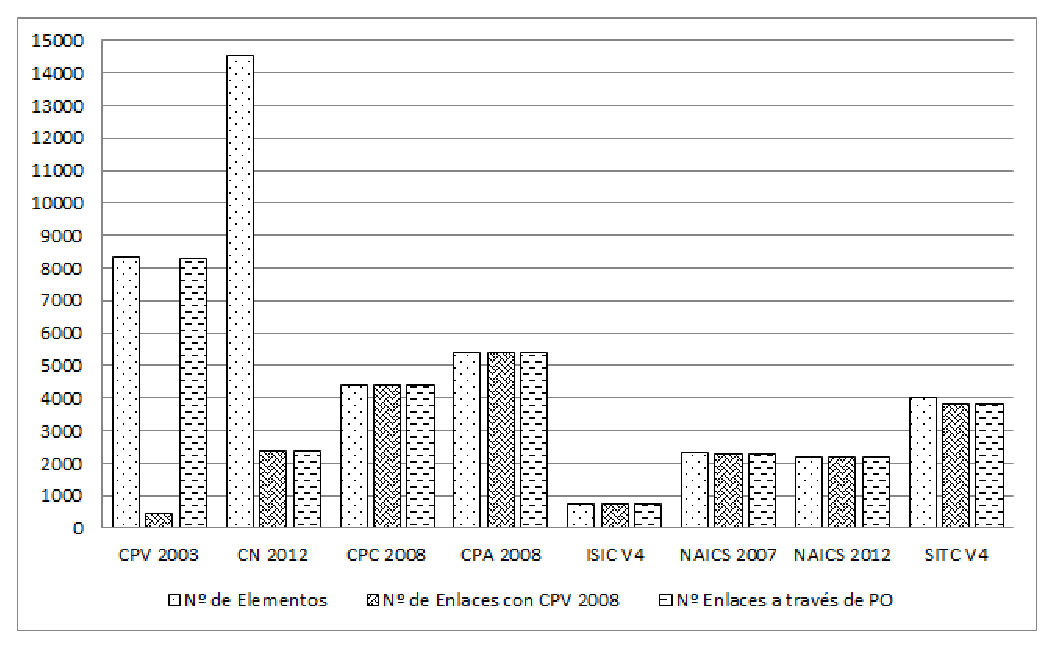
\includegraphics[width=14cm]{./images/phd/experimentation/pscs-enlaces}
\caption{Gráfica de Número de Elementos y Enlaces entre las PSCs y el CPV 2008.}
\label{fig:pscs-enlaces}
\end{figure}

\begin{figure}[!htb]
\centering
	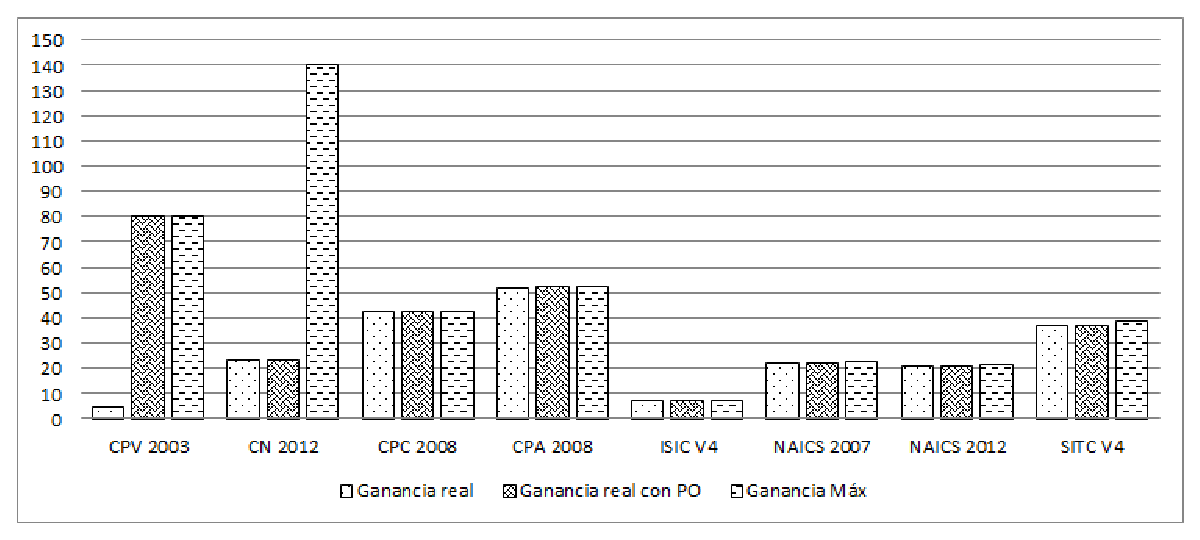
\includegraphics[width=14cm]{./images/phd/experimentation/pscs-ganancia}
\caption{Gráfica de Ganancia en expresividad.}
\label{fig:pscs-ganancia}
\end{figure}

\subsubsection{Punto de vista Cualitativo}
La ejecución de este experimento requiere la evaluación uno a uno de los criterios diseñados en las distintas 
tablas para su posterior evaluación. Para ello, se han acumulado en una hoja de cálculo las respuestas 
de cada uno de los enfoques y agregado todos los resultados en las Tablas~\ref{tabla:agregado-full} y~\ref{tabla:agregado-full-porcentaje}, 
también de forma gráfica en las Figuras~\ref{fig:eval-criteria-ppn},~\ref{fig:eval-criteria-pscs} y~\ref{fig:eval-criteria-orgs} se 
pueden observar los resultados obtenidos. De esta forma, se recoge por un lado 
la valoración y por otra la representación gráfica respecto al modelo de referencia. En el Apéndice~\ref{tablas-validacion-apen} se 
presenta la valoración para el modelo de referencia como ejemplo de evaluación y para la visualización del diseño de las 
tablas de validación.

\begin{sidewaystable}[ht!]
\renewcommand{\arraystretch}{1.3}
\begin{center}
\begin{tabular}{|p{3cm}||c|c|c||c|c|c||c|c|c||c|c|c||c|c|c||c|c|c||c|c|c||c|c|c|}
\hline
\textbf{Versión}&\multicolumn{3}{|c||}{$T^{1}$} & \multicolumn{3}{|c||}{$T^{2}$}& \multicolumn{3}{|c||}{$T^{3}$} & \multicolumn{3}{|c||}{$T^{3}_1$} & \multicolumn{3}{|c||}{$T^{4}$} & \multicolumn{3}{|c||}{$T^{4}_1$} & \multicolumn{3}{|c||}{$T^{5}$} & \multicolumn{3}{|c|}{$T^{6}$} \\ \hline
 &\si&\no&\na&	\si&\no&\na&	\si&\no&\na&	\si&\no&\na&	\si&\no&\na&	\si&\no&\na&	\si&\no&\na&	\si&\no&\na \\ \hline
 \textbf{Referencia} &\textbf{60}&\textbf{0}&\textbf{9}&	\textbf{44}&\textbf{0}&\textbf{0}&	\textbf{4}&\textbf{0}&\textbf{0}&	\textbf{5}&\textbf{0}&\textbf{0}&	\textbf{8}&\textbf{0}&\textbf{0}&	\textbf{14}&\textbf{0}&\textbf{0}&	\textbf{5}&\textbf{0}&\textbf{0}&	\textbf{33}&\textbf{0}&\textbf{14}\\ \hline \hline
  \multicolumn{25}{|c|}{\textbf{Anuncios de Licitación}} \\ \hline
 \textbf{\gls{TED}}	     			& 13 & 7 & 49 	& 0 & 0 & 44  	& 1 & 0 & 3  & 1 & 0 & 4  & 6 & 2 & 0  & 11 & 3 & 0  	& 0 & 0 & 5  & 0 & 0 & 47 \\ \hline
 \textbf{Plataforma de Contratación}	& 15 & 5 & 49 	& 0 & 0 & 44  	& 1 & 0 & 3  & 1 & 0 & 4  & 7 & 1 & 0  & 11 & 3 & 0  	& 0 & 0 & 5  & 0 & 0 & 47 \\ \hline 
 \textbf{\gls{BOE}}	     			& 10 & 9 & 50 	& 0 & 0 & 44  	& 1 & 0 & 3  & 1 & 0 & 4  & 8 & 0 & 0  & 10 & 3 & 1  	& 0 & 0 & 5  & 0 & 0 & 47 \\ \hline 
 \textbf{Servicios Externos}	     	& 12 & 8 & 49 	& 0 & 0 & 44  	& 1 & 0 & 3  & 1 & 0 & 4  & 5 & 3 & 0  & 6 & 3 & 5  	& 0 & 0 & 5  & 0 & 0 & 47 \\ \hline 
 \textbf{LOTED}	     			& 35 & 24 & 10 	& 23 & 8 & 13  	& 4 & 0 & 0  & 5 & 0 & 0  & 8 & 0 & 0  & 12 & 2 & 0  	& 5 & 0 & 0  & 0 & 0 & 47 \\ \hline 
 \textbf{\gls{MOLDEAS}}	     		& 54 & 7 & 8  	& 31 & 3 & 10 	& 4 & 0 & 0  & 5 & 0 & 0  & 8 & 0 & 0  & 14 & 0 & 0 	& 5 & 0 & 0  & 0 & 0 & 47 \\ \hline 
 \multicolumn{25}{|c|}{\textbf{Catálogo de Clasificaciones de Productos}} \\ \hline
 \textbf{\gls{CSV}/MSExcel} & 9 & 4 & 56 & 0 & 0 & 44 & 0 & 0 & 4 & 2 & 0 & 3 & 8 & 0 & 0 & 6 & 8 & 0 & 0 & 0 & 5 & 0 & 0 & 47 \\ \hline 
 \textbf{Servicios on-line} & 11 & 11 & 47 & 0 & 0 & 44 & 0 & 0 & 4 & 0 & 0 & 5 & 5 & 2 & 1 & 5 & 8 & 1 & 0 & 0 & 5 & 0 & 0 & 47 \\ \hline 
 \textbf{\gls{MOLDEAS}}& 54 & 7 & 8 & 31 & 3 & 10 & 4 & 0 & 0 & 5 & 0 & 0 & 8 & 0 & 0 & 14 & 0 & 0 & 5 & 0 & 0 & 32 & 0 & 15 \\ \hline 
 \multicolumn{25}{|c|}{\textbf{Organizaciones}} \\ \hline
 \textbf{TED} 			&  3 & 3 & 63 & 0 & 0 & 44 & 0 & 0 & 4 & 1 & 0 & 4 & 6 & 2 & 0 & 10 & 4 & 0 & 0 & 0 & 5 & 0 & 0 & 47 \\ \hline 
 \textbf{Plataforma de Contratación} &    13 & 4 & 52 & 0 & 0 & 44 & 1 & 0 & 3 & 1 & 4 & 0 & 8 & 0 & 0 & 12 & 2 & 0 & 0 & 0 & 5 & 0 & 0 & 47 \\ \hline 
 \textbf{\gls{BORME}}			 &    1 & 0 & 68 & 0 & 0 & 44 & 0 & 0 & 4 & 1 & 0 & 4 & 8 & 0 & 0 & 13 & 1 & 0 & 0 & 0 & 5 & 0 & 0 & 47 \\ \hline 
 \textbf{Servicios Externos} 	&  12 & 8 & 49 & 0 & 0 & 44 & 1 & 0 & 3 & 1 & 0 & 4 & 1 & 7 & 0 & 5 & 5 & 4 & 0 & 0 & 5 & 0 & 0 & 47 \\ \hline 
 \textbf{\gls{BBDD} externa} 		&     1 & 0 & 68 & 0 & 0 & 44 & 0 & 0 & 4 & 0 & 0 & 5 & 1 & 5 & 2 & 10 & 4 & 0 & 0 & 0 & 5 & 0 & 0 & 47 \\ \hline 
 \textbf{OpenCorporates} 	&    35 & 22 & 12 & 21 & 10 & 13 & 4 & 0 & 0 & 4 & 0 & 1 & 8 & 0 & 0 & 13 & 1 & 0 & 0 & 0 & 5 & 0 & 0 & 47 \\ \hline 
 \textbf{MOLDEAS} 		&    54 & 7 & 8 & 44 & 0 & 0 & 4 & 0 & 0 & 5 & 0 & 0 & 8 & 0 & 0 & 14 & 0 & 0 & 5 & 0 & 0 & 0 & 0 & 47 \\ \hline 
\hline
  \end{tabular}
  \caption{Tabla agregada de Validación Conjunta con Valores Parciales.}
  \label{tabla:agregado-full}
  \end{center}
\end{sidewaystable} 

\cleardoublepage

\begin{figure}[!htb]
\centering
	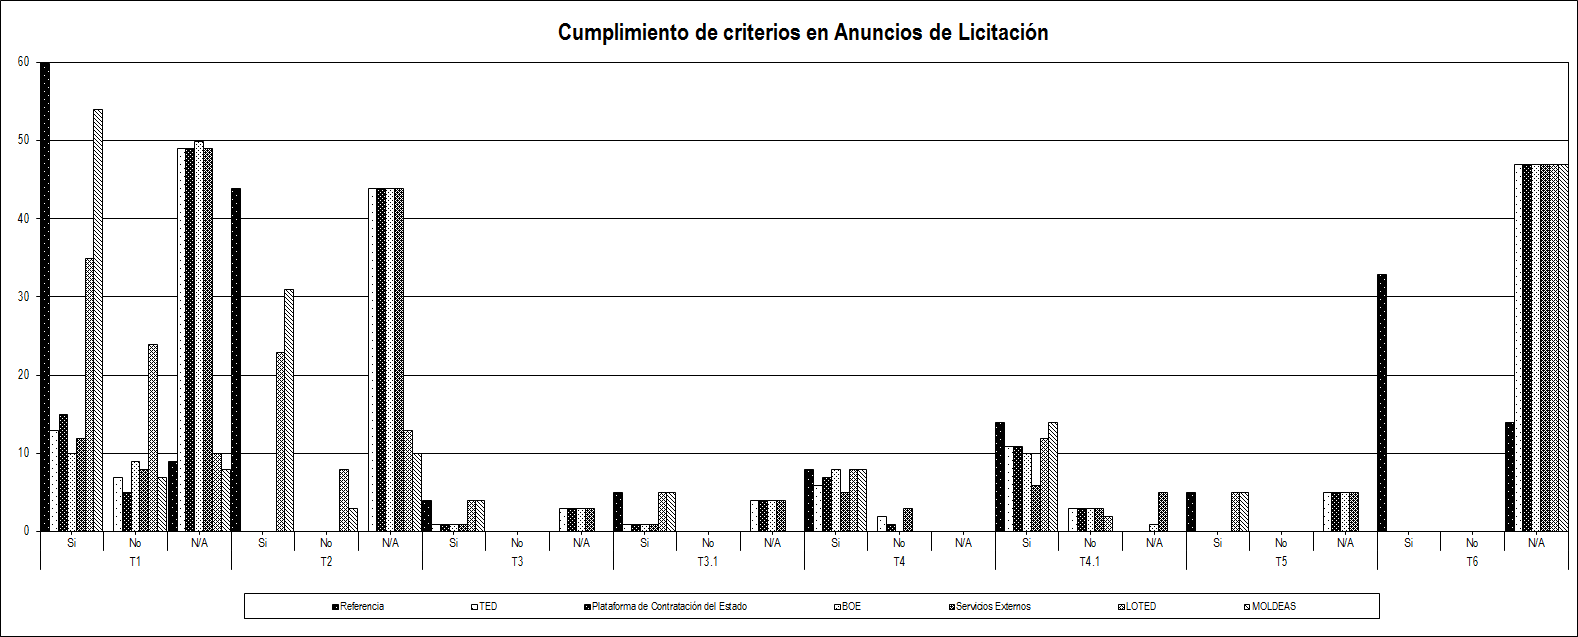
\includegraphics[width=16cm]{./images/phd/experimentation/criterios-ppn}
\caption{Gráfica del Grado de Cumplimiento de Criterios en Anuncios de Licitación.}
\label{fig:eval-criteria-ppn}
\end{figure}

\begin{figure}[!htb]
\centering
	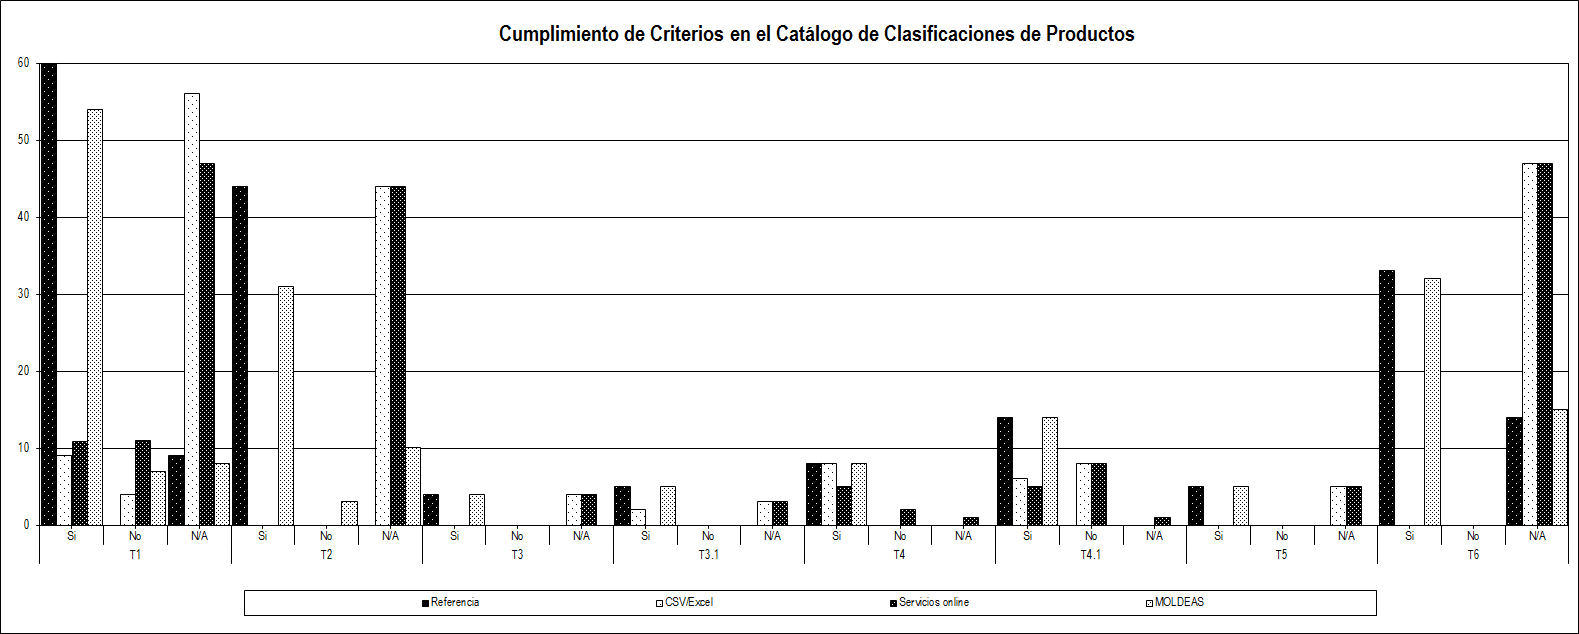
\includegraphics[width=16cm]{./images/phd/experimentation/criterios-pscs}
\caption{Gráfica del Grado de Cumplimiento de Criterios en el Catálogo de Clasificaciones de Productos.}
\label{fig:eval-criteria-pscs}
\end{figure}

\begin{figure}[!htb]
\centering
	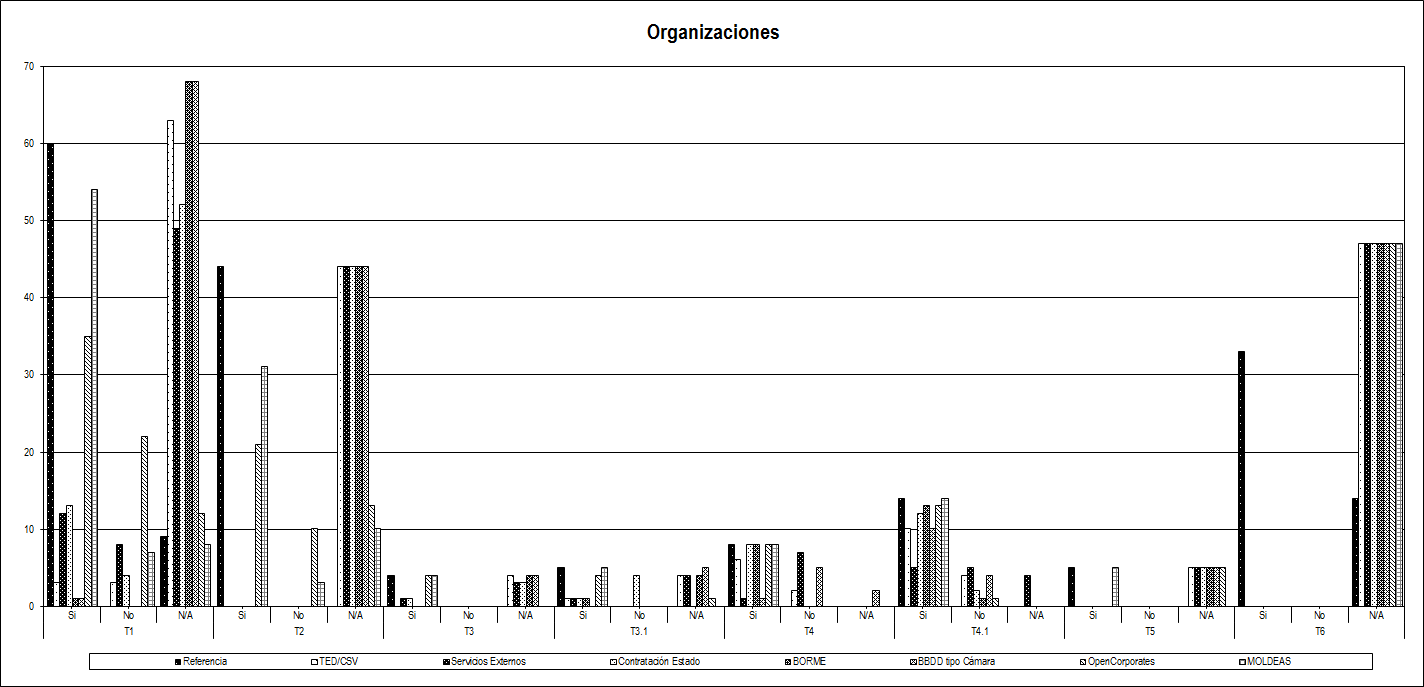
\includegraphics[width=16cm]{./images/phd/experimentation/criterios-orgs}
\caption{Gráfica del Grado de Cumplimiento de Criterios en las Organizaciones.}
\label{fig:eval-criteria-orgs}
\end{figure}

En la Tabla~\ref{tabla:agregado-sumatorio} se presenta la suma de todos los criterios para cada una de las tablas de validación, con el 
objetivo de ofrecer una visión simplificada de la evaluación. Con el objetivo de representar esta información de forma 
gráfica y poder realizar una comparación visual se han elaborado las siguientes gráficas tanto para los 
anuncios de licitación, ver Figura~\ref{fig:eval-criteria-1-ppn}, como para el catálogo de clasificaciones de productos, ver Figura~\ref{fig:eval-criteria-1-ppn}, y 
finalmente para la información y datos relativos a las organizaciones, ver Figura~\ref{fig:eval-criteria-1-orgs}.


\begin{longtable}[c]{|p{3cm}|c|c|c|c|c|c|c|c|}
\hline
\textbf{Versión}&$T^{1}$ & $T^{2}$& $T^{3}$ & $T^{3}_1$ & $T^{4}$ & $T^{4}_1$ &$T^{5}$ & $T^{6}$ \\ \hline
\endhead
 \multicolumn{9}{|c|}{\textbf{Anuncios de Licitación}} \\ \hline
 \textbf{TED}	     			& $65$ & \na & $100$ & $100$ & $75$ & $78,57$ & \na & \na \\ \hline
 \textbf{Plataforma de Contratación}	& $75$ & \na & $100$ & $100$ & $87,5$ & $78,57$ & \na & \na \\ \hline 
 \textbf{BOE}	     			& $52,63$ & \na & $100$ & $100$ & $100$ & $76,92$ & \na & \na\\ \hline 
 \textbf{Servicios Externos}	     	& $60$ & \na & $100$ & $100$ & $62,5$ & $66,66$ & \na & \na \\ \hline 
 \textbf{LOTED}	     			& $59,32$ & $74,19$ & $100$ & $100$ & $100$ & $85,71$ & $100$ & \na \\ \hline 
 \textbf{MOLDEAS}	     		& $88,52$ & $91,18$ & $100$ & $100$ & $100$ & $100$ & $100$ & \na \\ \hline 
 \multicolumn{9}{|c|}{\textbf{Catálogo de Clasificaciones de Productos}} \\ \hline
 \textbf{CSV/MSExcel} 			&$69,23$ & \na & \na & $100$ & $100$ & $42,86$ & \na & \na \\ \hline 
 \textbf{Servicios on-line}  		&$50$ & \na & \na & \na & $71,43$ & $38,46$ & \na & \na \\ \hline 
 \textbf{MOLDEAS}			&$88,52$ & $100$ & $100$ & $100$ & $100$ & $100$ & $100$ & $100$ \\ \hline 
 \multicolumn{9}{|c|}{\textbf{Organizaciones}} \\ \hline
 \textbf{TED} 				& $50$ & \na & \na & $100$ & $75$ & $71,43$ & \na & \na \\ \hline 
 \textbf{Plataforma de Contratación} 	& $76,47$ & \na & $100$ & $20$ & $100$ & $85,71$ & \na & \na\\ \hline 
 \textbf{BORME}			 	& $100$ & \na & \na & $100$ & $100$ & $92,85$ & \na & \na \\ \hline 
 \textbf{Servicios Externos} 		& $60$ & \na & $100$ & $100$ & $12,5$ & $50$ & \na & \na \\ \hline 
 \textbf{BBDD externa} 			& $100$ & \na & \na & \na & $16,67$ & $71,43$ & \na & \na \\ \hline 
 \textbf{OpenCorporates} 	 	& $61,40$ & $67,74$ & $100$ & $100$ & $100$ & $92,86$ & $100$ & \na\\ \hline 
 \textbf{MOLDEAS} 		 	& $88,52$ & $91,18$ & $100$ & $100$ & $100$ & $100$ & $100$ & \na \\ \hline 
\hline
  \caption{Tabla agregada de Validación Conjunta con Porcentajes \si entre aplicables.}
  \label{tabla:agregado-full-porcentaje}
\end{longtable} 



\begin{longtable}[c]{|l|c|c|c||c||c|} 
\hline
 \textbf{Versión} & \si&\no&\na & \textbf{Total} & \textbf{\% \si entre aplicables} \\\hline
\endhead
    \textbf{Referencia} & 173 & 0 & 23 & 196& 100 \\ \hline \hline
 \multicolumn{6}{|c|}{\textbf{Anuncios de Licitación}} \\ \hline   
     \textbf{TED} & 32 & 12 & 152 &$\equiv$ & $72.72$\\ \hline 
     \textbf{Plataforma de Contratación} & 35 & 9 & 152 &$\equiv$ & $79.54$\\ \hline 
    \textbf{BOE} & 30 & 12 & 154 &$\equiv$ & $71.42$\\ \hline 
    \textbf{Servicios Externos} & 25 & 14 & 157 &$\equiv$ & $64.10$\\ \hline 
    \textbf{LOTED} & 92 & 34 & 70 &$\equiv$ & $73.01$\\ \hline 
     \textbf{MOLDEAS} & 121 & 10 & 65 &$\equiv$ & $92.36$\\ \hline 
 \multicolumn{6}{|c|}{\textbf{Catálogo de Clasificaciones de Productos}} \\ \hline
    \textbf{CSV/MSExcel} &  25 & 12 & 159 &$\equiv$ & $67.56$\\ \hline 
     \textbf{Servicios on-line} &  21 & 21 & 154 &$\equiv$ & $50$\\ \hline 
    \textbf{MOLDEAS} &  166 & 7 & 23 &$\equiv$ & $93.86$\\ \hline 
 \multicolumn{6}{|c|}{\textbf{Organizaciones}} \\ \hline
    \textbf{TED} & 20 & 9 & 167 &$\equiv$ & $68.96$\\ \hline 
    \textbf{Plataforma de Contratación}  & 35 & 10 & 151 &$\equiv$ & $77.77$ \\ \hline 
    \textbf{BORME}  & 23 & 1 & 172 &$\equiv$ & $95.83$\\ \hline 
    \textbf{Servicios Externos}  & 20 & 20 & 156 &$\equiv$ & $50$\\ \hline   
    \textbf{BBDD externa}  & 12 & 9 & 175 &$\equiv$ & $57.14$\\ \hline 
    \textbf{OpenCorporates}  & 85 & 33 & 78  &$\equiv$ & $72.03$\\ \hline 
    \textbf{MOLDEAS}  & 121 & 10 & 65 &$\equiv$ & $92.36$\\ \hline 
\hline
\caption{Tabla agregada de Validación Conjunta con Valores Totales.}\label{tabla:agregado-sumatorio}\\    
\end{longtable}

\cleardoublepage

\begin{figure}[!htb]
\centering
	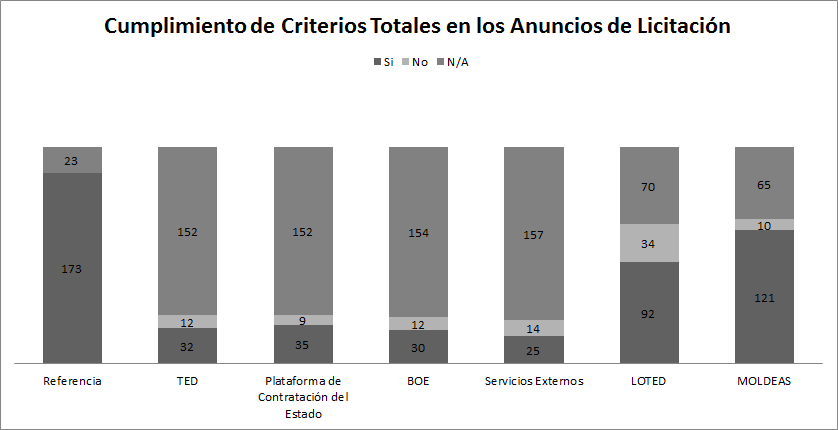
\includegraphics[width=12cm]{./images/phd/experimentation/criterios-total-ppn}
\caption{Gráfica del Grado de Cumplimiento Total de Criterios en Anuncios de Licitación.}
\label{fig:eval-criteria-1-ppn}
\end{figure}

\begin{figure}[!htb]
\centering
	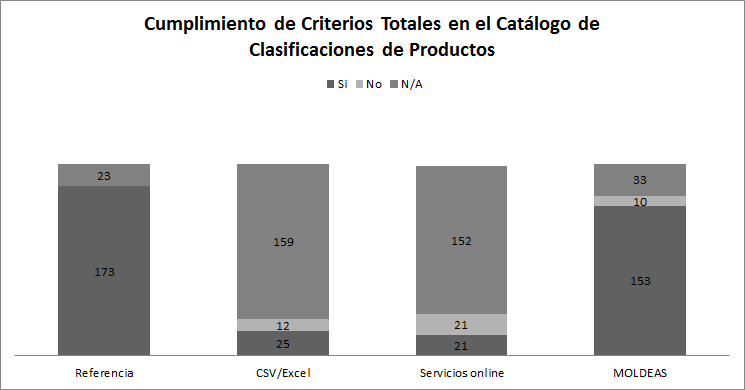
\includegraphics[width=14cm]{./images/phd/experimentation/criterios-total-pscs}
\caption{Gráfica del Grado de Cumplimiento Total de Criterios en el Catálogo de Clasificaciones de Productos.}
\label{fig:eval-criteria-1-pscs}
\end{figure}

\begin{figure}[!htb]
\centering
	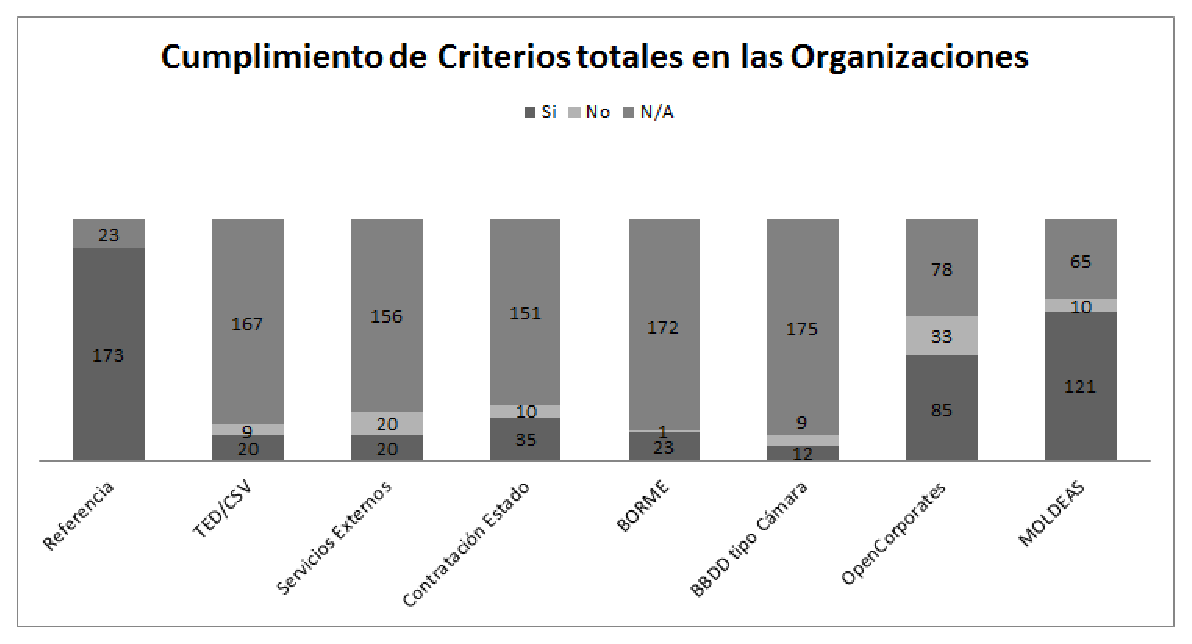
\includegraphics[width=14cm]{./images/phd/experimentation/criterios-total-orgs}
\caption{Gráfica del Grado de Cumplimiento Total de Criterios en las Organizaciones.}
\label{fig:eval-criteria-1-orgs}
\end{figure}


\subsection{Validación del experimento sobre la aplicación de \textit{Linked Data} a las Licitaciones Públicas}\label{sect:validation-tablas}


\subsubsection{Punto de vista Cuantitativo}\label{sect:experimento-pscs-validation}
El experimento diseñado y probado permite la verificación del porcentaje de ganancia al añadir y enlazar un vocabulario 
controlado con el \gls{CPV} 2008. La validación de este experimento debe plantearse asumiendo las siguientes premisas:
\begin{itemize}
 \item La selección del CPV 2008 como vocabulario matriz para el acceso a los anuncios de licitación pública 
en el ámbito de la Unión \gls{Europea}.
\item La condición de que todos los anuncios de licitación pública deben estar etiquetados obligatoriamente con 
este vocabulario.
\item La restricción de que el número de términos en el CPV 2008 es limitado.
\item La diferencia de recuperación de información entre un sistema basado en texto libre en contraposición con los 
basados en un vocabulario controlado.
\item La diversificación de vocabularios controlados, taxonomías, etc., existentes para el etiquetado de productos 
y servicios en diferentes ámbitos y con objetivos dispares: trazabilidad, extracción de estadísticas, etc.
\item La necesidad de realizar una combinación efectiva entre las clasificaciones de productos para asegurar
la comparación entre los mismos.
\item El número de documentos recuperados es completo si se utiliza todo el vocabulario del CPV 2008.
\end{itemize}

Bajo estas condiciones, el paradigma basado en \linkeddata permite que, a través de una correcta aplicación 
de un ciclo de vida para la generación de las clasificaciones de productos en \gls{RDF} y su enlazado posterior, 
se suministre el soporte necesario para cumplir con las premisas fijadas aumentando la capacidad expresiva 
del vocabulario de entrada para la recuperación de información de los anuncios de licitación pública en el 
ámbito europeo aumentando así la capacidad expresiva de los posibles clientes.

Desde el punto de vista del análisis de los resultados obtenidos y señalados en la sección anterior mediante la 
Tabla~\ref{ganancia-terminos} se pueden extraer las siguientes puntos clave:
\begin{itemize}
 \item La ganancia máxima ideal de expresividad se obtendrá cuando el vocabulario a añadir al conjunto de entrada 
contenga el mayor número de términos, es el caso de la clasificación de productos CN 2012. 
No obstante, el porcentaje de ganancia real dependerá siempre del número de términos que han sido enlazados 
al vocabulario matriz, en este caso el CPV 2008.
\item Hay que tener en cuenta que los enlaces generados desde una clasificación al CPV 2008 se encuentran 
bajo un umbral $\mu$ según el cual se admite la creación del enlace entre un concepto de una clasificación 
y el CPV 2008. Este umbral puede variar de una aplicación a otro y dependiendo del sistema de reconciliación 
de entidades utilizado será más o menos exacto. El objetivo reside en que la posibilidad de aumentar el vocabulario 
de entrada pudiendo realizar consultas bajo un determinado umbral $mu$ de concreción del enlace.
\item De todos los enlaces generados entre las clasificaciones de productos y el CPV 2008 $1503+462 = 1965$ son exactos 
porque han sido realizados por fuentes oficiales. Esto supone un incremento del $8.65\%$ y $6.64\%$ (a través de \textit{ProductOntology}) 
 en el número de términos nuevos posibles en el vocabulario de entrada perfectamente enlazados sin ningún umbral de ambig\"{u}edad, 
simplemente realizando su transformación a \linkeddata y creando los enlaces entre sí de forma automática. Los porcentajes 
restantes de $91.35\%$ y $93.36\%$ respectivamente indican enlaces automáticos, esta situación es habitual en el ámbito 
de \linkeddata y la única forma de decrementar estos valores consiste en la intervención manual para la validación 
de los enlaces con expertos del dominio.
\item Respecto a la ganancia en términos porcentuales se fija un máximo de $405.86\%$, un real $209.66\%$ y un real a través 
de \textit{ProductOntology} de $285.66\%$, lo que supone respectivamente un incremento de la expresividad de $5$, $3$ y cerca de 
$4$ veces más, en el número de nuevos términos a utilizar en el vocabulario de entrada debido al uso de \linkeddata respecto 
a la versión actual.
\item La selección de una nueva clasificación para ser enlazada con el CPV 2008 se debería basar en los siguientes criterios:
\begin{enumerate}
 \item Número de términos.
 \item Ganancia ideal y real.
\end{enumerate}

No obstante, se establece un nuevo parámetro consistente en el número de enlaces exactos que se pueden establecer 
entre el vocabulario a añadir y el matriz, facilitando así la comprobación de la calidad de la adición del nuevo 
vocabulario. Esta situación pese a que responde a un entorno ideal, la realidad es que en el ámbito de datos enlazados 
se trabaja bajo unos ciertos umbrales de incertidumbre que son admitidos por la propia comunidad. Evidentemente, dependiendo 
del tipo de aplicación este punto debe ser considerado en mayor o menor medida.

\item En cuanto al uso de un vocabulario intermedio como es \textit{ProductOntology} su uso se convierte en estratégico 
por su carácter internacional. En general, no existe una mejora excesivamente reseñable respecto al enlazado de términos 
directo o indirecto salvo en el CPV 2003, en el cual sólo se habían contemplado los enlaces exactos, y que supone 
un incremento del número de términos enlazados desde el $4.46 \%$ al $80.25 \%$. Esto implica que el proceso de enlazado inicial 
entre una clasificación y el CPV 2008 ha sido lo suficientemente bueno como para no ser necesario un paso intermedio mediante 
otro vocabulario que pudiera realizar el descubrimiento de nuevos enlaces.

\item Respecto al enlazado entre el \gls{CPV} 2008 y \textit{ProductOntology} si bien supone una ganancia apreciable en cuanto 
a expresividad de entrada, $10000$ nuevos términos posibles, simplemente se ha implementado y señalado pero no se considera estrictamente 
adecuado aunque aumente considerablemente la expresividad, ya que el vocabulario de entrada posible de \textit{ProductOntology} es $\inf$ por construcción del mismo, 
por lo que se prefiere su uso como puente entre una \gls{PSC} y el CPV 2008 y no se compara con las demás clasificaciones de productos en cuanto 
a características: vocabulario controlado, realizado por una entidad, etc.

\item Finalmente, es conveniente tener presente el problema de la recursión y posibilidad de convertir un vocabulario 
controlado de entrada (finito) en infinito por la suposición de nuevos enlaces entre elementos que directamente 
no están enlazados. Esta cuestión es perjudicial en dominios concretos y cerrados, como en el caso de los anuncios 
de licitación pública europea, pero si es beneficiosa (o admisible) en un entorno abierto para la realización de consultas 
de extracción de información sobre una base de datos infinita como es la Web, siempre teniendo presente el tiempo 
de la federación de consultas, etc., como se ha presentando en secciones anteriores

\end{itemize}

\subsubsection{Punto de vista Cualitativo}
El experimento y evaluación realizada permiten realizar una calificación y comparación entre los distintos enfoques 
disponibles para la publicación y acceso a la información y datos referente a los anuncios de licitación, incluyendo
el catálogo de clasificaciones de productos y las organizaciones. El diseño de las tablas, como se ha señalado, busca 
la valoración de criterios correspondientes a la iniciativa \linkeddata y \opendata. De esta forma, si las valoraciones 
son completas en términos de valores positivos para las Tablas $T^{3}$, $T^{3}_1$ y $T^{4}$ se puede asegurar 
que los datos evaluados cumplen todos los criterios para ser considerados datos enlazados y abiertos, además 
de situarse con la máxima valoración en el modelo de 5 $\star$. Teniendo en cuenta esta premisa, aquellos 
enfoques que se sitúen bajo estas premisas estarán facilitando el acceso a la información de los anuncios 
de licitación mediante la aplicación completa de estas iniciativas y por lo tanto, se puede asegurar que 
todos los beneficios y ventajas que se proponen bajo estos paradigmas se cumplen, por ejemplo los presentados en la Tabla $T^{4}_1$. Además de este valoración 
principal de los criterios de \linkeddata y \opendata se han propuesto otras tablas con el objetivo de 
validar la calidad de los datos producidos en el sentido de la información y metainformación que contienen, 
el modelo de producción y publicación utilizado y las facilidades de consumo de los datos suministradas, estas 
características se ven reflejadas en la Tabla $T^{1}$. Adicionalmente y al igual que en el diseño del \textit{software}, 
es conveniente la aplicación de patrones de diseño con el objetivo de resolver problemas comunes mediante un enfoque 
sistemático, esta cuestión conlleva la valoración de los patrones de diseño utilizados al modelar los datos enlazados y que 
se propone en la Tabla $T^{2}$. Finalmente, como uno de los puntos de clave para la difusión de los datos enlazados y 
cumpliendo la motivación inicial de esta iniciativa de reutilización de información, es importante la validación en 
cuanto a la posibilidad de pertenencia a la nube de datos enlazados, Tabla $T^{5}$, así como a los registros CKAN, Tabla $T^{6}$. Si 
bien los criterios de estas últimas tablas no son obligatorios en el sentido de \linkeddata, si que tienen una importancia 
capital cuando nos referimos a datos enlazados abiertos, ya que carece de sentido realizar un esfuerzo para la apertura 
y enlazado de datos si la meta final no reside en su posterior reutilización. 

A continuación se realiza una validación pormenorizada para cada uno de los conjunto de datos y enfoques 
evaluados, se ha agrupada la valoración respecto a las tablas realizadas ya que la justificación de los resultados 
es similar en cada uno de los conjuntos de datos:

\begin{enumerate}
 \item Atendiendo a las calificaciones de cada uno de los enfoques se puede observar 
como varios de los enfoques tienen características propias de los procesos implicados en la iniciativa de 
\linkeddata en cuanto a la publicación de datos y el diseño del acceso a la información a través de \gls{URI}s, de ahí 
que los distintos enfoques obtengan ciertos criterios positivos en la Tabla $T^{1}$ pese a que no se consideren
bajo el paradigma de datos enlazados. Sin embargo, el esfuerzo realizado en el proyecto LOTED se ve reflejado 
en un grado aceptable de cumplimiento de los criterios evaluados, la negatividad de otros queda justificada por la 
ausencia de metainformación en los \datasets. En el caso particular del enfoque propuesta por este trabajo, \gls{MOLDEAS}, 
las calificaciones son positivas en un grado muy alto debido a la aplicación de un ciclo de vida para la generación 
de datos enlazados como un proceso de ingeniería, no obstante los puntos negativos obtenidos se refieren a cuestiones 
relacionadas con la documentación adicional necesaria que debería ser labor del experto en el dominio y dirigida 
a diferentes usuarios (técnicos, finales, etc.).

\item En cuanto a la validación de acuerdo a los patrones de diseño presentes en la Tabla $T^{2}$, los enfoques que utilizan datos enlazados si reflejan 
la aplicación de los mismos, si bien no se considera necesario la aplicación de todos ellos, si es conveniente 
aplicarlos en la mayor medida posible. 

\item De nuevo la Tablas $T^{3}$, $T^{3}_1$ van dirigidas a los enfoques basados en datos enlazados principalmente, por lo que 
aquellos esfuerzos que no se encuentran bajo esta paradigma resultan ampliamente damnificados en su evaluación, cubriendo 
tan sólo alguna características básica. 

\item Sin embargo, la calificación de casi todos los enfoques en lo referente a los principios
de \opendata en la Tablas $T^{4}$, $T^{4}_1$ es verdaderamente positiva debido principalmente a la naturaleza de la información 
y datos que es intrínsecamente abierta. Aquellos enfoques que ofrecen servicios de negocios se ven penalizados debido a que 
utilizan datos abiertos pero su estrategia o política posterior con los mismos restringe su uso y tan sólo cumplirán estos 
requisitos si los servicios de suscripción fueran libres respecto a la información, manteniendo su coste respecto al servicio 
construido sobre los datos, por ejemplo análisis, predicción o estadísticas. Evidentemente, esta situación sería ideal y también 
deben obtener rentabilidad del coste de recuperación de información.

\item Las Tablas $T^{5}$, $T^{6}$ son orientadas nuevamente a las iniciativas basadas en datos enlazados ya que carecen 
de sentido para las demás debido a su naturaleza. En este sentido, tanto los enfoques realizados por MOLDEAS y LOTED son 
candidatos a pertenecer a la nube de datos enlazados y a los registros \gls{CKAN} sin ningún tipo de inconveniente.

\end{enumerate}

En general, la tendencia que se observa en las tablas es que la información y datos relativa a los anuncios de licitación, 
clasificaciones de productos y organizaciones tiene un carácter abierto, como confirman los resultados, e incluso disponen
de buenos fundamentos para que la realización del esfuerzo de transformación a datos enlazados sea asumible tanto 
por las Administraciones Públicas como por terceros, así lo demuestra el trabajo presentado en este documento 
a través del enfoque realizado en \gls{MOLDEAS}. La aplicación de los principios de \linkeddata y \opendata permiten 
asegurar ventajas y beneficios en el acceso a la información y manejo de los datos tanto para las personas físicas 
como para los componentes software, facilitando su consumo y permitiendo impulsar la creación de nuevos servicios 
de valor añadido con la información relevante de los anuncios de licitación y su entorno. De esta manera, el esfuerzo 
realizado por las empresas actuales de recuperar información de fuentes de datos heterogéneas y con distintos 
formatos como \gls{PDF}, \gls{HTML}, etc., es altamente mitigado debido al uso de datos enlazados.

\subsection{Evaluación del experimento sobre la aplicación de \textit{Linked Data} a las Licitaciones Públicas}


\subsubsection{Punto de vista Cuantitativo}
La ejecución y validación del experimento del uso de datos enlazados en la recuperación de información de 
los anuncios de licitación aumentando la expresividad del vocabulario de entrada (\gls{CPV} 2008) permite 
dar respuesta las preguntas establecidas en el diseño del experimento.

\begin{itemize}
 \item ¿Cuál es la expresividad actual, en términos de número de conceptos para realizar consultas, 
para el acceso a la información de anuncios de licitación?

La versión inicial y los sistemas disponibles en Internet hacen uso del vocabulario CPV 2008 para la creación de consultas 
sobre los anuncios de licitación disponiendo de una expresividad como vocabulario de entrada de $10357$ términos. Debido 
a que este vocabulario es normativo a nivel europeo en el sentido de que cualquier anuncio de licitación debe 
contener al menos un código CPV 2008, se puede establecer que utilizando el conjunto completo de términos del vocabulario 
de entrada se puede acceder a la base documental completa de los anuncios de licitación, independientemente de la tecnología 
utilizada.

\item ¿Cuál es la ventaja de uso de un modelo \gls{RDF} para la expresión y recuperación de la información de los anuncios de licitación?

Además de las ventajas intrínsecas del uso de RDF y la realización práctica del enfoque de \linkeddata sobre las clasificaciones 
de productos y la información de los anuncios de licitación pública europea, el principal beneficio reside en el enlazado de datos 
desde otro vocabulario de entrada al CPV 2008 permitiendo el incremento el número de términos del vocabulario de entrada que inicialmente 
sólo contiene a los términos del CPV 2008 y mediante esta técnica se incrementa notablemente, aumentando el universo del discurso para 
la recuperación de información de los anuncios de licitación. 

 \item ¿Cómo los datos enlazados favorecen el aumento de expresividad en la ejecución de consultas y por tanto facilitan la recuperación de los 
anuncios de licitación? 

Según la respuesta realizada en la pregunta anterior y la validación presentada en la Sección~\ref{sect:experimento-pscs-validation}, el uso 
de datos enlazados beneficia la creación de consultas enriquecidas respecto al vocabulario de entrada permitiendo al cliente la utilización 
de un mayor número de términos convirtiendo el conocimiento del CPV 2008 en opcional. En la validación realizada y con la transformación 
de las clasificaciones de productos realizadas se obtiene un incremento entre $3$ y $4$ veces más respecto al 
número de términos posibles iniciales provenientes del CPV 2008, la evolución del número de términos se puede observar en 
la Figura~\ref{fig:eval-n-terminos}.

\begin{figure}[!htb]
\centering
	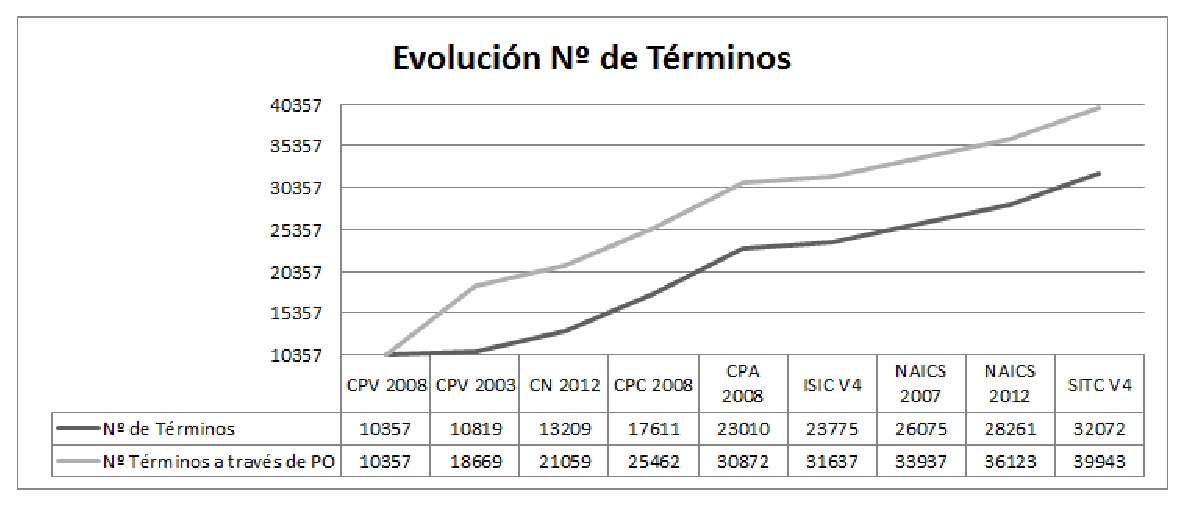
\includegraphics[width=14cm]{./images/phd/experimentation/evo-n-terminos}
\caption{Evolución Número de Términos.}
\label{fig:eval-n-terminos}
\end{figure}



\item ¿Cuál es el beneficio real del uso de datos enlazados para representar la información? 

El beneficio real reside en la representación de información y datos mediante un modelo estándar (\gls{RDF}) que permite el uso 
de lenguajes (\gls{SPARQL}) y protocolos (\gls{HTTP}) estándar para su acceso facilitando la recuperación de información. Evidentemente, 
el contraste respecto a las actuales versiones en \gls{HTML}, \gls{PDF}, MSExcel, etc., y sistemas de recuperación opacos suministradores 
por proveedores que generan servicios de negocio sobre ellos, es crítico, ya que simplemente el manejo de información 
de distintas fuentes y formatos requiere un esfuerzo que se solventa en gran medida con el uso de datos enlazados. Es necesario 
resaltar que el enfoque realizado en este documento es posible debido a la posibilidad de utilizar \opendata y mejorar éstos 
con la iniciativa de \linkeddata. Adicionalmente, se estable una fórmula para el cálculo de la ganancia al introducir 
una nueva clasificación enlazada con el \gls{CPV} 2008.

\item ¿Se incurre en algún error al aumentar la expresividad?

El enlazado de datos consta de una variable de incertidumbre que si bien es aceptada por la comunidad, debe ser tenida en cuenta 
para la realización de aplicaciones de carácter crítico. En este sentido y siguiendo con la validación realizada, al menos, 
se obtiene un incremento entre el $6.64\%$ (con \textit{ProductOntology}) y $8.65\%$ exacto del vocabulario controlado 
de entrado. En el caso particular de recuperación de documentos estos porcentajes son muy relevantes pero incluso 
la introducción de términos ``relacionados'' bajo un umbral de incertidumbre es conveniente ya que el funcionamiento 
del sistema se mantiene y se aumenta la expresividad de entrada para la realización de consultas. Por todo ello, 
pese a que este problema de enlazado de recursos y reconciliación de entidades está asociado a la iniciativa de 
\linkeddata, sólo se puede solventar con el esfuerzo de expertos en el dominio con el consiguiente coste. 

\end{itemize}

En resumen, el enfoque seguido en este experimento y en el estudio de este documento es extrapolable a un entorno o dominio en el cual exista un vocabulario 
controlado para la recuperación de documentos, existan diferentes vocabularios provenientes de distintas fuentes 
candidatos a interoperar con el inicial y en consecuencia a servir para el aumento del universo de discurso en 
ese dominio.


\subsubsection{Punto de vista Cualitativo}
La ejecución y validación del experimento del grado de cumplimento de criterios referentes a datos enlazados abiertos permite 
dar respuesta a las preguntas planteadas en el diseño del experimento.

\begin{itemize}
 \item ¿El ciclo de vida seguido y los datos generados certifican la aplicación de buenas prácticas de \linkeddata?

A la vista de la evaluación realizada de los distintos enfoques ha quedado patente que en la actualidad tanto la información 
como los datos disponibles son abiertos en su mayor parte e incluso son utilizados para la construcción de servicios 
comerciales pero el esfuerzo requerido para llevar a cabo estos productos se ve reflejado en el precio de los mismos. La aplicación 
de los principios de \linkeddata puede rebajar ampliamente este coste de acceso a la información promoviendo la 
competitividad y creando una administración más transparente. En este sentido el trabajo realizado en \gls{MOLDEAS} partiendo 
de la definición de un ciclo de vida (procesos, métodos y tareas) y del conjunto de datos referente al dominio de 
\eproc permite asegurar los criterios de \linkeddata además de cumplir las características más 
deseables en cuanto producción, publicación y consumo de datos.

 \item ¿El ciclo de vida seguido y los datos generados certifican el cumplimiento de los principios de \opendata?

De la misma forma que en la pregunta anterior el modelo de ciclo de vida seguido ha permitido conservar el carácter 
de datos abiertos intrínseco la información y datos relativa al entorno de los anuncios de licitación como se ha reflejado 
en las tablas de validación referentes a \opendata.

 \item ¿Qué nivel del modelo de 5 $\star$ se puede establecer?

Consecuentemente por la aplicación del ciclo de vida y las valoraciones realizadas en los criterios relativos al nivel 
dentro del modelo de 5 $\star$ se refleja la consecución de la calificación más alta. En este punto cabe realizar una reflexión 
sobre el nivel de estrellas que deben tener los datos abiertos enlazados, especialmente los referentes a las Administraciones Públicas. En muchos 
casos y especialmente desde un punto de vista de un desarrollados es suficiente la publicación de datos a través de \gls{RSS} (3 $\star$), esta situación 
es consecuencia directa de la simplicidad de este formato tanto en representación como por su madurez, ahora bien, la publicación de datos 
bajo 5 $\star$ confiere nuevas cualidades a los mismos como un modelo formal subyacente, la posibilidad de reconciliación automática, realización 
de procesos de razonamiento, etc., que para aplicaciones de gestión de la información avanzada resultan de gran interés. En conclusión, 
desde un punto de vista práctico el nivel de 3 $\star$ sería suficiente pero las ventajas adicionales de los datos 5 $\star$ debe conducir 
a una valoración por parte de los propietarios de datos a exigir este nivel aunque el esfuerzo inicial sea mayor la recompensa a medio/largo 
plazo debe ser superior, más aún teniendo en cuenta la tendencia actual de apertura y enlazado de datos en diferentes dominios. 

 \item ¿Qué porcentaje de patrones de diseño se han aplicado en los datos generados?

Los patrones de diseño en disciplinas como la Ingeniería de \textit{Software} permiten dar solución a problemas comunes de una 
forma sistemática y probada. En muchas ocasiones el exceso de uso de patrones implica añadir una complejidad extra 
a un determinado \textit{software} para el cual ya se ha fijado una fecha de caducidad, viéndose así 
 su capacidad de extensión es cercenada desde el inicio. Con ello, se pretende ejemplificar que si bien la complejidad 
de introducir patrones de diseño en el dominio del \textit{software} requiere un esfuerzo permite obtener beneficios 
posteriores. En el caso de los datos enlazados ocurre de la misma forma, además de ofrecer una solución a problemas comunes también pretende 
que el calado y la perduración en el tiempo de los datos enlazados sea la mayor posible facilitando así 
su reutilización. Es por ello que en MOLDEAS se ha aplicado el mayor número de patrones posible siempre teniendo presente 
la valoración del coste/beneficio y la no obligatoriedad de aplicación, de esta forma se puede fijar un porcentaje de uso en $X\%$.

 \item ¿Los datos generados pueden pertenecer a la nube de datos enlazados abiertos?

De acuerdo a los resultados en la evaluación tanto los datos particulares concernientes a los anuncios de licitación 
como los del catálogo de las clasificaciones de productos y las organizaciones son candidatos a formar parte 
de la nube de datos enlazados. Hasta el momento y como resultado colateral a este trabajo el catálogo de 
clasificaciones de productos ya ha sido incluido formalmente en la nube de datos enlazados, los referentes a 
los anuncios de licitación y las organizaciones debido a que han sido cedidos por la empresa Gateway S.C.S 
dentro de la ejecución del proyecto ``10ders Information Services'' se ha pospuesto su inclusión oficial.

 \item ¿Los datos generados pueden pertenecer a un registro CKAN? 

En conjunción a la respuesta de la pregunta anterior la metainformación necesaria para pertenecer a este tipo 
de registro está disponible para cada uno de los \dataset \gls{RDF}, por lo que es posible realizar el registro en cualquier 
portal de datos enlazados basado en \gls{CKAN}.

 \item ¿Se puede asegurar que los datos son enlazados y abiertos?

La evaluación realizada en las Tablas $T^{3}$, $T^{3}_1$ y $T^{4}$ verifica que se cumplen los requisitos, principios y criterios 
necesarios para que los datos realizados en bajo \gls{MOLDEAS} sean considerados como abiertos y enlazados.


 \item ¿Qué beneficios se obtienen del cumplimiento de estos objetivos?

El enfoque realizado en MOLDEAS trasciende más allá de la simple transformación de datos siguiendo unas directrices, se ha 
establecido un ciclo de vida perfectamente definido que permite la gestión eficaz de la información y de los datos consiguiendo 
que un proceso considerado dramático, en algunos casos, se convierta en un proceso de ingeniería cuantificable. Es por ello que 
además de las ventajas inherentes a los datos enlazados abiertos es necesario añadir los propios generados del trabajo realizado 
en este estudio. En particular y desde un punto de vista de los datos enlazados abiertos se destacan los siguientes 
beneficios:
\begin{itemize}
  \item Mejora en el acceso a la información y datos, integración de distintas fuentes de datos, servicios de acceso 
basados en lenguajes formales.
 \item Aumento de la visión global de los datos, expresividad y estructuración.
 \item Aplicación intensiva de estándares.
 \item Incremento del conocimiento en el dominio de la contratación pública electrónica.
 \item Creación de un proceso de gestión del ciclo de vida de los datos enlazados.
 \item Impulso de la reutilización de la información y datos, mayor poder de redistribución
 \item Minimización de restricciones tecnológicas. Impulso de la reutilización automática.
 \item Minimización de aspectos discriminatorios en el uso de la información y de los datos.
 \item Aumento de la transparencia, inclusión y responsabilidad, mayor conocimiento de la información 
de procedencia.
\item Incremento en la concienciación de los avances en la gestión e integración de datos.
\item Alineación con las actuales propuestas estratégicas de futuro.
\item \ldots
\end{itemize}

\end{itemize}



\section{Experimento sobre el Sistema MOLDEAS}
\section{Introducción}
En el caso objeto de estudio de este documento se ha planteado la aplicación de los principios 
de \linkeddata, para el modelado y explotación de datos e información provenientes de los anuncios de 
licitación públicos. Para ello, tal y como se ha presentado en los anteriores capítulos, se ha definido 
un ciclo de vida de datos enlazados que a través de procesos, métodos y tareas suministra una metodología 
de actuación genérica para proceder en este sentido. Como ejemplo de su validez y aplicación se han utilizado 
los datos de los contratos públicos para ejemplificar los procesos de producción, publicación, consumo, validación y 
actualización, ver Figura~\ref{fig:com}. Aunque ciertas tareas se apoyan en el uso de aplicaciones de terceros como Google Refine o bien 
en la parametrización de bibliotecas ya existentes como Apache Lucene, es necesario suministrar un entorno 
en el cual los resultados de aplicación de las tareas puedan ser procesados para implementar algunas de las ya 
especificadas y así ejemplificar transversalmente el uso de datos enlazados en un determinado dominio. Por ello y 
de acuerdo al análisis y especificación realizado se plantea la necesidad de diseñar los componentes del sistema 
MOLDEAS como paso final para la cobertura en el uso de datos enlazados en el campo de la contratación pública 
electrónica y teniendo presentes los siguientes objetivos:

\begin{itemize}
 \item Facilitar y dar soporte a las tareas del ciclo de vida que no puedan ser desarrolladas completamente 
por herramientas externas.
\item Validar los datos generados por otras herramientas.
\item Enriquecer con procesos \textit{ad-hoc} la información y datos de los anuncios de licitación según el modelo 
y especificación fijado en el Capítulo~\ref{capitulo:metodos-separados}.
\item Implementar un demostrador público de consumo de datos enlazados.
\item Proveer un sistema de búsqueda/recomendación de anuncios de licitación de acuerdo a criterios predefinidos 
por el cliente.
\item Establecer un conjunto de prueba que realice la validación parcial de ciertos procesos apoyándose en tecnología 
pre-existente.
\item Diseñar un sistema extensible y escalable para su futura ampliación.
\end{itemize}

\begin{figure}[h]
\centering
\begin{tikzpicture}
  \path[mindmap,concept color=gray,text=white]
    node[concept] {MOLDEAS}
    [clockwise from=0]
    child[concept color=gray!65!black] {
      node[concept] {moldeas-api}   
      [clockwise from=-90]
      child [concept color=gray!60] { node[concept] {\textbf{Consumo}} }   
    }  
    child[concept color=gray!65!black] {
      node[concept] {moldeas-transformer}
      [clockwise from=-90]
      child [concept color=gray!60] { node[concept] {\textbf{Producción}} }
      child [concept color=gray!60] { node[concept] {\textbf{Publicación}} }           
    }
    child[concept color=gray!65!black] { node[concept] {moldeas-test} 
      [clockwise from=-90]
      child  [concept color=gray!60] { node[concept] {\textbf{Validación}} }      
    }
    child[concept color=gray!65!black] { node[concept] {moldeas-common} } ;
   
\end{tikzpicture}
    \caption{Alineación inicial de componentes de MOLDEAS y procesos del Ciclo de Vida de \linkeddata.}
 \label{fig:com}
\end{figure}

Ante estos objetivos de gran envergadura, teniendo en cuenta el ciclo de vida de datos enlazados definido y las tareas 
especificadas para la información y datos presentes en las licitaciones públicas, cabe especificar el diseño 
de los componentes del sistema MOLDEAS como elemento vertebrador tanto de los procesos como de la información. De esta forma, 
a lo largo de este capítulo se realiza una descripción del diseño e implementación realizada en el sistema MOLDEAS haciendo 
especial hincapié en los detalles más relevantes del mismo.
\section{Descripción del Sistema MOLDEAS}
La tarea de análisis de un sistema conlleva la especificación de una serie 
de requisitos que guíen el posterior diseño e implementación del sistema 
\gls{MOLDEAS}. De esta forma, se pueden extraer los siguientes objetivos: 
\begin{itemize}
 \item Analizar e identificar el trabajo relacionado.
 \item Identificar y definir los requisitos asociados a las actividades de investigación, 
innovación y desarrollo a realizar.
 \item Especificar los requisitos de usuario para los distintos componentes
 \item Realimentar los puntos anteriores con los resultados obtenidos.
\end{itemize}

Estos objetivos ya han sido parcialmente cubiertos en los anteriores 
capítulos, en los cuales se ha repasado intensivamente la mayoría de los 
trabajos relacionados y relevantes en el dominio de la contratación 
pública electrónica así como se ha puesto de manifiesto los procesos, 
métodos y tareas a desarrollar dentro del ciclo de vida de datos 
enlazados. Es por ello que este capítulo se centrará en presentar las partes más relevantes y 
destacadas del sistema MOLDEAS y su aplicación en las distintas 
tareas del ciclo de vida así como en el desarrollo del sistema de búsqueda 
de anuncios de licitación. En primer lugar, cabe mostrar un esbozo del 
sistema con una vista funcional del mismo, ver Figura~\ref{fig:functional-overview}, en el cual 
se enclavan los distintos procesos del ciclo de vida y los objetivos generales del sistema: 
producción de datos enlazados de los anuncios de licitación para su posterior 
almacenamiento y publicación a través de un \textit{endpoint} de \gls{SPARQL} y un \linkeddata \textit{frontend} y 
consumo de los datos almacenados para la construcción de servicios de valor añadido como el 
sistema de búsqueda/recomendación de anuncios de licitación. Se ha optado por enfoque 
totalmente práctico en este capítulo de ingeniería con el objetivo de resaltar y documentar la innovación del sistema 
MOLDEAS sin focalizar en metodologías intensivas de ingeniería del \textit{software}.


\begin{figure}[!htb]
\centering
	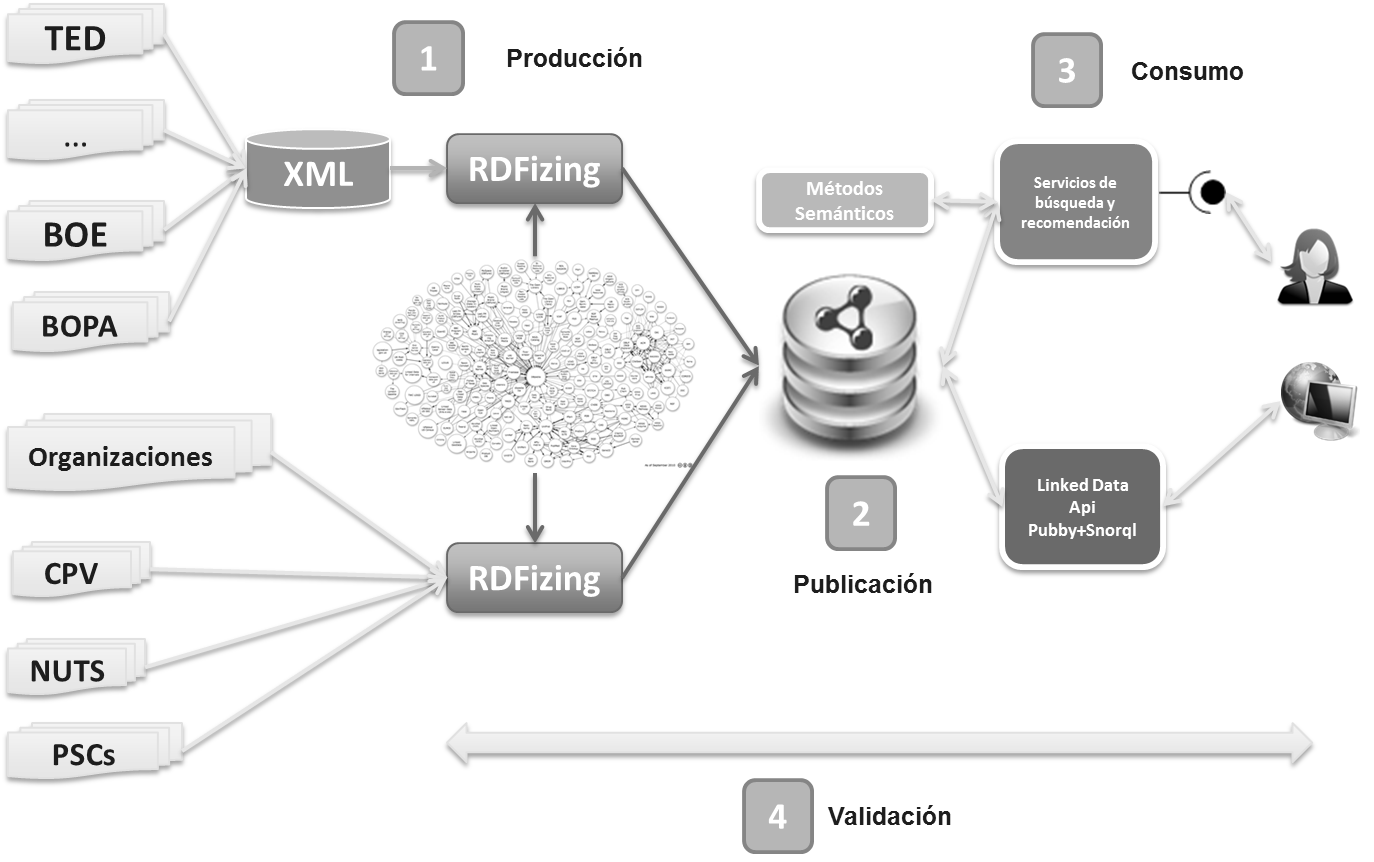
\includegraphics[width=12cm]{images/phd/moldeas/functional-overview}
\caption{Arquitectura funcional del sistema MOLDEAS.}
\label{fig:functional-overview}
\end{figure}

A la vista de la arquitectura funcional propuesta, se ha realizado una aproximación en distintos componentes, 
de acuerdo a sus responsabilidades e interacciones, ver Figura~\ref{fig:moldeas-components}, y con la siguientes 
definiciones:

\begin{description}
 \item [moldeas-common.] Alberga utilidades necesarias a lo largo de todos los procesos del ciclo de vida de datos 
enlazados.
 \item [moldeas-transformer.] Se encarga de dar soporte a la producción de datos enlazados cubriendo las tareas de transformación, 
  enriquecimiento, reconciliación de entidades, etc.  
 \item [moldeas-api.] Se encarga del consumo de los datos enlazados publicados bajo unas 
ciertas características en un \textit{endpoint} de SPARQL y que con la aplicación de varios 
métodos de expansión de consultas es capaz de generar consultas SPARQL cercanas al lenguaje natural 
para la recuperación de los anuncios de licitación.
\item [moldeas-test.] Se encarga de la validación de los datos enlazados y de los métodos de expansión definidos en \texttt{moldeas-api}.
 \item [moldeas-web.] Se encarga de la presentación y consumo de datos enlazados suministrando 
un interfaz gráfico para \texttt{moldeas-api} en el cual el usuario puede seleccionar las 
características de los anuncios de licitación para su posterior búsqueda y 
presentación con diferentes vistas (tabla, mapa, etc.). Además, suministra un interfaz de servicios REST para el acceso 
a los métodos disponibles en \textit{moldeas-api} por lo que cumple una doble función: 1) servir como demostrador 
público para el usuario y 2) ejemplificar las llamadas a \texttt{moldeas-api} desde un punto de vista 
del desarrollador.
\end{description}

\begin{figure}[!htb]
\centering
	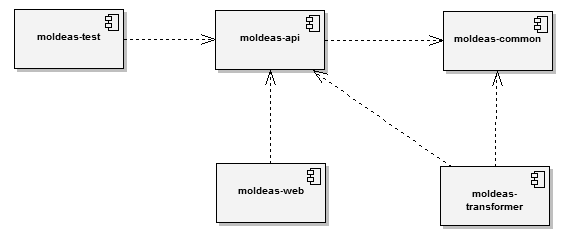
\includegraphics[width=12cm]{images/phd/moldeas/moldeas-componentes}
\caption{Componentes del sistema MOLDEAS.}
\label{fig:moldeas-components}
\end{figure}

\subsection{Arquitectura de alto nivel}
%Diagramas de componentes, diagramas de paquetes
El despliegue de una infraestructura de datos enlazados requiere la cooperación de diferentes elementos 
\textit{hardware} y \textit{software}. Según el análisis realizado de cada uno de los componentes un diagrama 
de despliegue de la arquitectura propuesta en MOLDEAS se presenta en la Figura~\ref{fig:moldeas-despliegue}. 
La descripción de cada uno de estos nodos y componentes es la siguiente:

\begin{itemize}

\item Nodo web. En el cual se encuentran disponibles un servidor web \gls{HTTP} como es Apache2 HTTP Server, este elemento \textit{software} sirve como punto 
de entrada a los elementos del sistema, tanto para el consumo de datos enlazados directamente por otras máquinas como para las peticiones 
relativas al componente \textit{moldeas-web}. También, se utiliza este servicio para albergar una aplicación 
de ejecución de consultas \textit{on-line} en SPARQL como \gls{SNORQL}, sin necesidad de utilizar directamente 
el interfaz propuesto por el \textit{endpoint} de SPARQL.

\item Nodo de aplicaciones web. En el cual se encuentra instalado un contenedor de aplicaciones web \gls{J2EE} como Apache Tomcat, 
con el objetivo de albergar las aplicaciones relativas al \linkeddata \textit{frontend} y a la aplicación \textit{moldeas-web}. 

\item Nodo repositorio RDF. En el cual se instala el repositorio \gls{RDF}, en el cual se almacenan y publican 
los datos enlazados provenientes de los anuncios de licitación. La publicación de datos enlazados se realiza a través de su almacenamiento 
en un repositorio RDF nativo como Virtuoso de OpenLink, suministrando adicionalmente un \textit{endpoint} SPARQL para que los 
datos puedan ser reutilizados y consumidos tanto por la propia aplicación de \textit{moldeas-api} como por clientes 
de forma externa, en este caso se por el \linkeddata \textit{frontend} y SNORQL.

\end{itemize}

Físicamente estos nodos y componentes se han diseñado de forma separada ya que la comunicación entre los mismos 
se realiza mediante delegación de consultas y comunicación mediante HTTP. De esta manera, se permite que el sistema 
sea escalable y flexible, pudiendo sustituir el entorno tecnológico seleccionado por otros proveedores.

Los componentes especificados en MOLDEAS tienen un doble carácter ya que algunos son utilizados de forma \textit{off-line} como 
es el caso de \texttt{moldeas-transformer} y \texttt{moldeas-test}, específicamente para los procesos de producción y validación 
de datos enlazados, mientras que otros como \textit{moldeas-web} sirven como cliente de los servicios proporcionados 
en \texttt{moldeas-api} de forma \texttt{on-line}. Transversalmente \textit{moldeas-common} se utiliza a lo largo de cualquier 
ejecución ya que contiene las clases \textit{Helper} necesarias para la ejecución de tareas comunes.

\begin{figure}[!htb]
\centering
	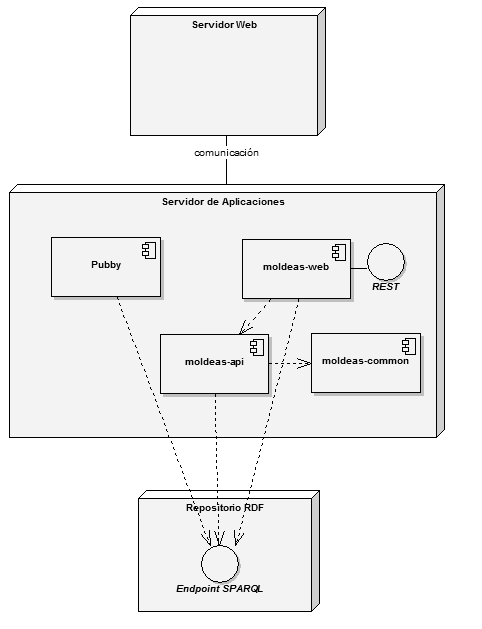
\includegraphics[width=12cm]{images/phd/moldeas/moldeas-despliegue}
\caption{Diagrama de Despliegue de MOLDEAS.}
\label{fig:moldeas-despliegue}
\end{figure}

\subsection{Entorno Tecnológico}
En el momento de analizar y diseñar un conjunto de componentes \textit{software} es necesario seleccionar aquellas 
bibliotecas y herramientas que suministren determinadas funcionalidades de base. La selección estratégica 
de esta tecnología y herramientas se describe someramente a continuación:

\begin{itemize}
 \item Lenguaje de programación Java 1.6. En el campo de la Web Semántica y en particular de la iniciativa de 
datos enlazados, la mayoría de las bibliotecas y funcionalidades externas se encuentran programadas 
en este lenguaje, por lo que unido a la experiencia propia del autor la decisión de uso de este lenguaje 
queda perfectamente justificada.
\item Apache Maven2. El desarrollo de aplicaciones debe realizarse de forma sostenible, es por ello que esta herramienta da 
soporte a todo el proceso de construcción de software: compilación, pruebas, empaquetado, despliegue, documentación, ejecución, etc. 
Además de proveer los mecanismos apropiados para la gestión de dependencias de forma declarativa. 
\item Eclipse \gls{IDE}. La edición del código fuente de las clases Java se ha realizado a través de este entorno de desarrollo, ampliamente 
asentado en la comunidad Java y con una excelente comunidad que proporciona herramientas extra a través de distintos 
\textit{plugins}, proporcionando un entorno productivo y con altas capacidades para el desarrollador. Adicionalmente, Maven 
es capaz de generar a través de su fichero de configuración la estructura de un  proyecto de Eclipse de forma automática.
\item Repositorio de código fuente. Se ha seleccionado la forja de proyectos de Google Code para albergar los cambios y las actualizaciones 
maduras a través del sistema de control de versiones Mercurial.
\item Jena 2.6.4. Biblioteca Java de base tecnológica para la Web Semántica que incluye las principales funciones para el tratamiento de \gls{RDF}, \gls{OWL}, etc. 
así como facilita la ejecución de consultas \gls{SPARQL} tanto de forma local (en memoria) como distribuida (en un \textit{endpoint}).
\item Log4j 1.2.14. Biblioteca Java para la gestión del sistema de registro de una aplicación mediante la cual se puede especificar 
los distintos niveles de registro así como la serialización de los mismos.
\item Junit 4.0. \textit{Framework} Java para la ejecución de pruebas unitarias con un amplio abanico de configuraciones y extras 
para el diseño de pruebas de integración, regresión, etc.
\item Apache \gls{Lucene} 2.9.0. Motor de búsqueda sintáctica en Java con amplias posibilidades tanto para el indexado de documentos, procesamiento 
de lenguaje natural y ejecución de consultas.
\item Apache \gls{Solr} 1.4.1. Plataforma empresarial de búsqueda en Java basada en Apache Lucene que añade nuevas funcionales como nuevos 
filtros para el procesamiento de lenguaje natural.
\item Apache \gls{Mahout} 0.4. Biblioteca Java con un amplio espectro de algoritmos de \textit{data mining} y aprendizaje automático, con capacidades 
para integrarse con otras herramientas como Apache Hadoop y que propone un framework extensible para la creación de nuevos algoritmos.
\item Spring 2.5. \textit{Framework} Java para la creación de aplicaciones empresariales basado en la técnica inversión de control y el uso 
de \textit{Plain Old Java Object} (\gls{POJO}s) para el diseño flexible y el desarrollo ágil de \textit{software}.
\item Jersey \gls{REST} 0.8. Biblioteca Java para la creación de servicios web REST mediante anotaciones.
\item Jquery 1.4.1. \textit{Framework} para el desarrollo de interfaces de usuario enriquecidos basados en HTML+CSS+Javascript.
\item Exhibit 2.2.0. Biblioteca basada en Javascript para el desarrollo de interfaces con múltiples vistas para la presentación 
de datos en general.
\item \gls{Pubby} 0.3.3. \linkeddata \textit{frontend} para la negociación de contenido y presentación de datos enlazados disponibles 
a través de un \textit{endpoint} de \gls{SPARQL}.
\item \gls{SNORQL}. Aplicación basada en HTML+Javascript para la realización de consultas \textit{on-line} sobre \textit{endpoints} de SPARQL.

\end{itemize}




















\section{Consideraciones Generales de Diseño}
En un sentido amplio, dado un problema y un dispositivo en el cual resolverlo, es necesario suministrar un método preciso de respuesta a la casuística 
planteada en el problema de acuerdo al dispositivo objetivo, a tal método se denomina \textit{algoritmo}. El diseño de algoritmos\cite{Vallecillo} 
tiene dos componentes importantes:

\begin{enumerate}
  \item El primero se refiere a la búsqueda de métodos o procedimientos, secuencias
finitas de instrucciones adecuadas al dispositivo del cual se dispone, que permita resolver el problema.  
\item  El segundo permite medir de alguna forma el coste (en tiempo y recursos) de consumo de un algoritmo con el fin de encontrar la
solución, ofreciendo la posibilidad de comparar distintos algoritmos que resuelven un mismo problema.
\end{enumerate}

Una vez que se dispone de un algoritmo que funciona correctamente, es necesario
definir criterios con el objetivo de medir su rendimiento o comportamiento. Estos criterios se centran principalmente en su 
simplicidad y en el uso eficiente de los recursos. La sencillez es una característica sensiblemente interesante en el diseño 
de algoritmos, facilitando su verificación, el estudio de su eficiencia y el mantenimiento. De ahí que muchas veces se priorice la simplicidad y legibilidad 
del código frente a alternativas más crípticas y eficientes del algoritmo. Por otra parte, el uso eficiente de los recursos suele medirse en función de dos
parámetros: el \textit{espacio}, es decir, memoria utilizada, y el \textit{tiempo}, unidades de tiempo de ejecución. En ambos casos, 
se hace referencia a los costes que supone la búsqueda de la solución al problema planteado mediante un algoritmo, además estos dos parámetros 
son utilizados para una posible comparación ulterior de los algoritmos entre sí.

El tiempo de ejecución de un algoritmo dependerá de diversos factores como los datos de entrada que le suministremos, la calidad del código
generado por el compilador para crear el programa objeto, la naturaleza y rapidez de las instrucciones máquina del procesador concreto que ejecute el programa, y la
complejidad intrínseca del algoritmo.  Existen dos tipos posibles de estudio sobre el tiempo:

\begin{enumerate}
\item  Áquel que proporciona una medida teórica (a priori), consistiendo en la obtención de una función que acote 
(inferior o superiormente) el tiempo de ejecución del algoritmo para unos valores de entrada determinados.
\item  El qué ofrece una medida real (a posteriori), consistiendo la medición del tiempo de ejecución del algoritmo para unos valores de entrada determinados 
y un entorno de ejecución particular.
\end{enumerate}

Ambas medidas son importantes puesto que si bien la primera nos ofrece estimaciones
del comportamiento de los algoritmos de forma independiente del ordenador en donde serán implementados y sin necesidad de ejecutarlos, 
la segunda representa las medidas reales del comportamiento del algoritmo. 

\subsection{Consideraciones Diseño de Programas}\label{consideraciones-diseno}
El objetivo de implementación del sistema \gls{MOLDEAS} recae en suministrar parcialmente soporte 
a los distintos procesos implicados en el ciclo de vida de datos enlazados, 
si bien algunas tareas se realizan mediante el uso de ciertas herramientas, existen otras que deben ser parametrizadas e implementadas 
para ofrecer un entorno homogéneo para el manejo de la información y datos 
provenientes de los anuncios de licitación. La separación de responsabilidades 
entre los distintos componentes se realiza de acuerdo a su funcionalidad, de esta manera 
es posible realizar cambios transparentes en los componentes sin que los otros sean 
involucrados en el proceso de cambio: implementación, prueba y empaquetamiento. Por ello, 
se han definido los interfaces de comunicación entre los mismos como un API para que 
cualquier futuro desarrollo se apoye en este \textit{framework} para añadir nuevas 
funcionalidades. Las claves para un diseño abierto de un \gls{API} 
coinciden en muchos sentidos con los de un lenguaje de programación \cite{Interpretes}:

\begin{description}
\item[Concisión notacional:] el API deberá proporcionar un entorno con un nivel
de detalle adecuado: interfaces claras, simples, unificadas etc. Las posibles 
ampliaciones sobre el \textit{framework} de \textit{MOLDEAS} deben resultar sencillas
y no presentar inconvenientes para el programador comprender y extender su diseño.

\item[Ortogonalidad:] la funcionalidad del API debe suministrar el mecanismo
adecuado para combinar nuevos componentes y rechazar algunos de los ya
presentes. Por ejemplo la adición de nuevas restricciones no debe suponer una
recodificación del código del algoritmo.

\item[Abstracción:] el diseño del API debe basarse en el uso de técnicas como
los patrones de diseño e interfaces favoreciendo la abstracción de algoritmos.

\item[Seguridad:] los algoritmos implementados debe tener puntos obligatorios de restricciones
para verificar por ejemplo su terminación aunque se añadan nuevas
restricciones. 

\item[Expresividad:] el API debe ser lo suficientemente ``rica'' como para que
nuevas ampliaciones puedan ser formuladas de forma sencilla de acuerdo a la información 
y datos presentes en los anuncios de licitación y en su modelo formal. 

\item[Extensiblidad:] el API debe basarse en técnicas de programación que
favorezcan la adición de nuevas características y su adaptación para nuevas
configuraciones del algoritmo


\item[Portabilidad:] el lenguaje seleccionado para proporcionar estas técnicas
debe poseer esta característica.

\item[Eficiencia:] en cualquier implementación de un algoritmo o conjunto de los mismos esta característica es fundamental y
aunque el API diseñado, atendiendo a las características anteriores pueda
sobrecargar la ejecución básica de los procesos, su penalización en tiempo no es tan alta 
como para descartar los principios de diseño anteriores.

\item[Librerías e interacción con el exterior:] la ejecución de las funcionalidades 
provistas deberá ser independiente del lenguaje de ontologías utilizado, así aislamos el
conjunto de técnicas de la fuente de conocimiento favoreciendo el uso del
cualquier lenguaje de formalización.

\item[Entorno:] para facilitar la depuración de los algoritmos realizados se
proveerá un entorno gráfico en el cual poder visualizar la ejecución.
\end{description}

Además de estas principios generales para el diseño del API, hay que tener en
cuenta: 

\begin{itemize}
  \item El entorno de ejecución puede ser una aplicación web, por lo que, se
  deberá tener en cuenta en el diseño para que pueda fácilmente integrarse con
  \textit{frameworks} como Spring.
  \item La mayoría de las aplicaciones utilizando Web Semántica utilizan el
  lenguaje Java, por lo tanto, este será el lenguaje seleccionado en su última versión.
\end{itemize}
 
\subsection{Patrones de Diseño}\label{patrones}
Con el objetivo de cumplir los criterios antes mencionadas, el sistema \gls{MOLDEAS} se basará en la aplicación 
intensiva de patrones de diseño\cite{Gamma,CoreJ2EEPatterns} como buena práctica 
de programación. Normalmente estos patrones indican la interacción que ha de realizarse entre los distintos elementos 
que participan en el problema. De esta manera para cada problema tendremos un 
conjunto de objetos, cada uno de los cuales realizará una función proveyendo servicios a 
los demás objetos implicados. Los patrones de diseño proponen soluciones con distintas características: 
elegantes, modulares, escalables y flexibles. Una posible definición de los mismos 
se presenta a continuación:

\begin{Frame}
Los patrones de diseño representan soluciones para problemas recurrentes en la ingeniería del \textit{software}.
\end{Frame}

En general, se trata de soluciones estándar para un problema habitual en programación que utiliza 
distintas técnicas para la flexibilización del código intentando al mismo tiempo satisfacer 
ciertos criterios no funcionales. Se suelen asimilar a una estructura determinada de implementación 
que cumple una finalidad determinada y permite describir ciertos aspectos de un programa.

No obstante, pese a que los patrones nos ofrecen buenas soluciones puede darse el caso de que 
resulte contraproducente el uso de los mismos. El uso de estas técnicas debe realizarse, 
por tanto, en el momento justo. La problemática reside en establecer cuándo su aplicación 
es adecuada y se pueden citar varios criterios:
\begin{itemize}
    \item El código del programa ha crecido exponencialmente.
    \item Las clases de un programa aglutinan código semánticamente no corresponde con su funcionalidad.
    \item Se deben realizar pruebas unitarias de clases.
    \item El diseño del programa es altamente complejo y las relaciones entre las distintas 
clases es opaca.
   \item La comunicación con otros desarrolladores ha decaído debido a la complejidad del código.
\end{itemize}

El libro \textit{The Ganf of Four(Gof)}~\cite{Gamma} fue el pionero en introducir estas técnicas de 
programación caracterizando las mimas en tres niveles:
\begin{description}
    \item [Patrones creacionales:]se utilizan para la creación, inicialización
    Podemos destacar: \textit{Abstract Factory}, \textit{Builder}, \textit{Factory Method}, \textit{Prototype} o
    \textit{Singleton}.
    \item [Patrones estructurales:]su objetivo es separar la interfaz de
    operaciones de la implementación. Tratan de organizar cómo las clases y
    objetos se agrupan para generar estructuras y organizaciones más grandes.
    Por ejemplo: \textit{Adapter}, \textit{Bridge}, \textit{Composite}, \textit{Decorator} o \textit{Facade}.
    \item [Patrones de comportamiento:] describen la comunicación entre los
    objetos.  \textit{Chain of Responsability}, \textit{Command}, \textit{State}, \textit{Strategy} o \textit{Visitor} son
    ejemplos de este conjunto.
\end{description}

En combinación con los patrones de diseño, se encuentra la técnica de \textit{refactoring}~\cite{Fowler1999}, 
utilizada para reestructurar y refinar el código fuente (en muchos casos aplicando un determinado patrón) 
sin alterar la funcionalidad o comportamiento externo del mismo.




\section{Diseño de Componentes del Sistema MOLDEAS}
\subsection{Diseño de \texttt{moldeas-common}}\label{sect:moldeas-common}
El objetivo de este módulo es aunar aquella funcionalidad y lógica 
de negocio común a todos los procesos del ciclo de vida. De esta forma y 
atendiendo al modelo de construcción de aplicaciones Java propuesto 
por Maven se pueden separar responsabilidades entre los distintos 
componentes, compilar y empaquetar (como fichero \gls{JAR}) por separado las distintas clases 
de Java de manera transparente.

Entre las funcionalidades entregadas en este paquete hay que destacar 
las siguientes:
\begin{itemize}
 \item Clases para la carga de ontologías y de documentos RDF desde distintas 
fuentes de datos como ficheros o un \textit{endpoint} de \gls{SPARQL}. 

El doble objetivo de diseño de estos paquetes es: 1) independizar la ejecución de los procesos de la base de conocimiento 
y 2) abstraer la localización  (local, remoto, base de datos, etc.) y contenido del recurso.

Para diseñar estos dos objetivos se han seguido los siguientes criterios:
\begin{enumerate}
  \item El patrón \textit{\gls{DAO}} que sirve como guía para este primer objetivo, abstrayendo
  las operaciones necesarias sobre la base de conocimiento a un interfaz que
  pueda ser implementado por distintos proveedores.
  \item El segundo objetivo, se obtiene factorizando la
  información invariante de los recursos: el contenido del recurso puede ser siempre un
  \textit{InputStream} y todo recurso podrá ser localizado por un identificador
  único (nombre fichero, \gls{URL} o un id. de una base datos), no obstante para
  facilitar la abstracción de la clave de un recurso se ha diseñado como un
  objeto (\textit{KnowledgeResourcePK}) anticipando la necesidad de claves más
  complejas que una simple cadena identificativa. 
\end{enumerate}

En la Figura \ref{fig:moldeas-loading}, se realiza un diagrama de clases del módulo de acceso
a la base de conocimiento.

\begin{figure}[!htb]
\centering
	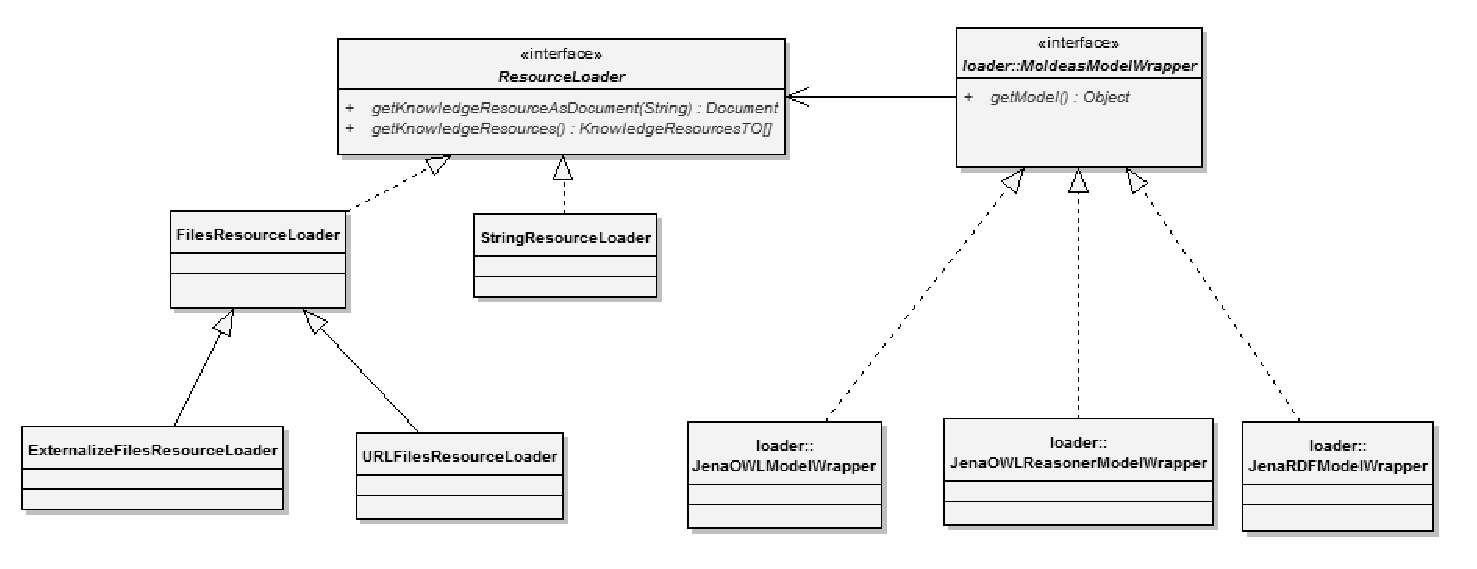
\includegraphics[width=16cm]{images/phd/moldeas/moldeas-loading}
\caption{Diagrama de Clases del acceso a datos (ontologías y RDF) en MOLDEAS.}
\label{fig:moldeas-loading}
\end{figure}


Uno de los puntos clave para facilitar un soporte escalable a los distintos lenguajes, 
consiste en la selección del \gls{API} para trabajar con ontologías y recursos RDF, para ello y teniendo 
en cuenta el uso del lenguaje de ontologías OWL y su representación bajo el modelo 
de datos RDF en sus distintos formatos, se debe realizar una abstracción que permita procesar 
la información y los datos con comodidad, ocultando los detalles de representación sintáctica 
y ofreciendo las abstracciones básicas de \gls{OWL} y \gls{RDF}: sentencias, sujeto, recurso, clases, 
propiedades, etc. En este sentido, las alternativas disponibles se centran en:

 \begin{description}    
  \item[Jena:] biblioteca Java de referencia para el trabajo en el 
campo de la Web Semántica conteniendo múltiples funcionalidades para el desarrollo 
de aplicaciones basadas en RDF y OWL. Se trata de \textit{software libre} 
inicialmente desarrollado por \textit{HPLabs} y actualmente bajo la fundación Apache.

\item[OWL-API:] es una biblioteca para Java específicamente diseñada para tratar ontologías expresadas en OWL. 
Se distribuye bajo licencia de \textit{software} libre y ha sido creada como parte del proyecto europeo 
\textit{WonderWeb}, en la actualidad es gestionada en la Universidad de Manchester. 

\item [Protégé-OWL-API:] utilizada en el IDE Protégé para el desarrollo de ontologías en OWL. Combina aspectos
 tanto de OWL-API como de Jena, no obstante, su ámbito está más orientado hacia a este editor que como biblioteca 
para un usuario programador.         
\end{description}

Una vez valoradas las posibilidades de estas herramientas, se ha seleccionado Jena ya que proporciona soporte 
para el tratamiento de varios lenguajes y formatos de modelado, permite la integración con herramientas 
y procesos externos como los razonadores, y además su comunidad ha crecido exponencialmente 
en los últimos tiempos gracias a su adhesión al proyecto Apache, lo que le confiere un grado 
de madurez y confianza extra que asegura un correcto funcionamiento de la misma.


\item Clases para el almacenamiento de constantes a lo largo del ciclo de vida 
de los datos manejados por el sistema \gls{MOLDEAS}. En este sentido, es conveniente parametrizar 
los valores de las \gls{URI}s base, los grafos RDF, así como los prefijos y espacios de nombres 
de todos los vocabularios y \datasets reutilizados. Esta práctica evita los errores 
ortográficos en la codificación de URIs tanto en la producción de datos como en su consumo 
a través de consultas SPARQL o mediante el propio API definido por Jena.


\item Clases para la gestión de errores y excepciones que se puedan producir a lo largo de cada uno de los procesos 
del ciclo de vida. El diseño de la gestión de errores es uno de los elementos importantes para la
robustez de un producto \textit{software}. Las directrices que se han seguido en MOLDEAS 
para el control de errores es el uso de las excepciones, para ello, se ha creado 
una simple jerarquía de excepciones que capture los posibles errores dentro de la aplicación. 
Se han considerado dos tipos de excepciones, ver Figura~\ref{fig:diagramas/excepciones}:
\begin{description}
\item[Excepciones no chequeadas:]  controlan errores graves producidos en tiempo
de ejecución e inesperados en el modelo. 
\item[Excepciones chequeadas:] controlan errores graves que se pueden producir
en tiempo de ejecución. 
\end{description}


\begin{figure}[htb]
\centering
	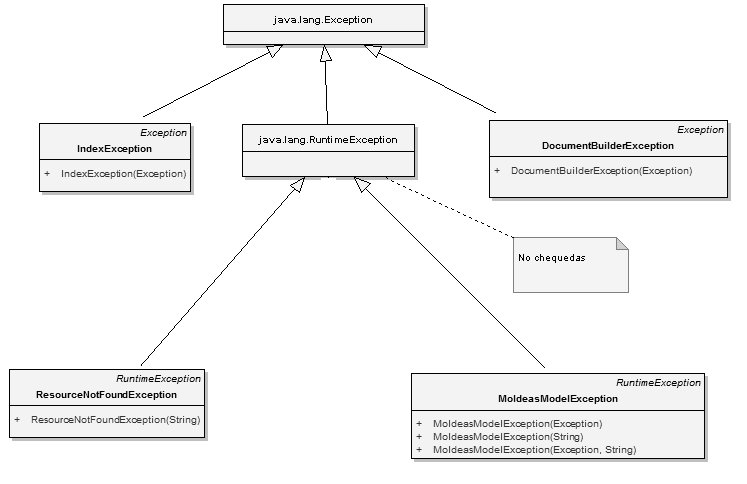
\includegraphics[width=16cm]{images/phd/moldeas/excepciones}
\caption{Diagrama Clases de excepciones en el sistema MOLDEAS.}
\label{fig:diagramas/excepciones}
\end{figure}

\item Clase para la configuración del registro y traza de la aplicación. Esta característica de verdadero valor para una aplicación, 
permite agilizar los procesos de depuración y su integración en sistemas de mayor calado. En todas las clases del sistema MOLDEAS candidatas a 
generar mensajes de registro, se ha utilizado la biblioteca \textit{Log4j} para la gestión del registro de la aplicación. Se trata de una herramienta 
Java para la gestión del registro y traza de acuerdo a un serie de 
niveles: \textit{DEBUG, INFO, WARN, ERROR y FATAL}. Esta división por niveles 
permite configurar los mensajes del sistema dependiendo del estado 
en el que se encuentre: desarrollo, depuración, producción, etc.

\item Otras clases de utilidad para acciones transversales como la carga de documentos 
\gls{XML}, ejecución de consultas \gls{SPARQL}, filtros de lenguaje natural para las bibliotecas 
de Apache \gls{Lucene} y \gls{Solr}.

\end{itemize}

\subsection{Diseño de \texttt{moldeas-transformer}}\label{sect:moldeas-transformer}
El objetivo de este módulo es facilitar el soporte al proceso específico 
de producción de datos enlazados para las distintas entidades de información 
provenientes de los anuncios de licitación. En el enfoque de este trabajo 
se han tenido en cuenta los datos a transformar y promocionar a la iniciativa 
de \linkeddata para agilizar las distintas tareas del modelo de ciclo 
de vida de datos enlazados propuestos. Existen ciertas tareas 
que se pueden acometer directamente con las herramientas existentes como 
Google \gls{Refine}, para las que su funcionamiento es correcto cuando 
los datos son homogéneos y tan sólo requieren la ejecución de una serie 
de \textit{mapeos} o reglas de transformación para utilizar los datos 
de entrada como valores en las tripletas \gls{RDF} a generar. Sin embargo, 
dependiendo del tamaño del \dataset de entrada a transformar, de la homogeneidad 
del mismo y de las operaciones posteriores a realizar como la adición de metainformación, 
la reconciliación de entidades o la simple serialización del modelo RDF en distintos 
formatos, hace necesario la implementación de un proceso personalizado que ejecute 
estas tareas de forma específica, ya que la dificultad de expresarlas en las herramientas 
de propósito general las convierte en tremendamente complicadas. Es por ello, que se han diseñado 
e implementado en este módulo una serie de funcionalidades de carácter específico 
para cada una de las entidades a transformar, teniendo presentes las características 
de las mismas. Para ello, se han considerado los siguientes puntos:

\begin{itemize}
 \item La transformación de la información propia de los anuncios de licitación conlleva la promoción 
de una gran cantidad de datos, que pueden ser tomados de distintas fuentes 
como fichero \gls{CSV}, MSExcel, \gls{XML} o desde una base de datos. En este sentido, 
y debido a dos variables importantes, el tamaño del \dataset y la diversidad 
de los formatos de entrada, se ha optado por la implementación de una serie de adaptadores 
que permiten procesar la información de entrada de forma homogénea de modo que la generación 
en RDF se convierte en un proceso transparente de la fuente de datos y se puede asegurar 
la validez de los datos transformados. En cuanto a la reconciliación de entidades, para este 
conjunto de datos no se considera necesaria ya que se realiza específicamente en el catálogo 
de clasificaciones de productos, sin embargo el enriquecimiento del \dataset de entrada si 
se ve afectado, ya que se han añadido nuevas propiedades (latitud y longitud) a los códigos NUTS para facilitar 
posteriores procesos como el de búsqueda de anuncios de licitación. 

Por tanto, los anuncios de licitación se transforman mediante un proceso Java \textit{ad-hoc} que cubre 
todas las tareas del ciclo de vida referentes a la producción de datos enlazados.

\item En cuanto al catálogo de clasificaciones y teniendo en cuenta las características de las mismas, 
tamaño relativamente pequeño y formato de entrada homogéneo, se ha optado por un enfoque híbrido, en el cual 
en el primer paso se realiza la transformación de los datos originales mediante la herramienta Google 
Refine de forma que una vez obtenidos los datos en RDF se realiza una serie de pasos específicos para la 
reconciliación de entidades (enlazado de las distintas clasificaciones con el CPV 2008) y la adición 
de metainformación. Para ello, se ha implementado un proceso Java capaz de tomar como fuente de datos 
RDF e ir accediendo y enriqueciendo cada una de las descripciones de productos y servicios disponibles, 
basándose en la construcción de un reconciliador de entidades específico con las bibliotecas de 
Apache \textit{Lucene} y \textit{Solr}.


\item Por último y en los datos particulares de organizaciones, países y personas se ha utilizado 
de nuevo un enfoque híbrido en el cual para la transformación inicial se ha optado por la herramienta 
de Google Refine, enriqueciendo y añadiendo a los datos RDF ya generados, las tripletas de información 
necesarias para cumplir con la especificación de recursos RDF realizada.

\end{itemize}

En general, este módulo consta de una serie de procesos independientes que son capaces, para cada una 
de las grandes entidades de información provenientes de los anuncios de licitación pública, de procesar 
los datos en distintos formatos, realizar el proceso de reconciliación de entidades y enriquecer los 
\datasets de entrada mediante la adición de metainformación. 


\subsection{Diseño de \texttt{moldeas-api}}\label{sect:moldeas-api}
Atendiendo a las consideraciones generales sobre diseño, se explicarán 
las decisiones de diseño más relevantes para la construcción 
de un \gls{API} que provee los métodos necesarios para el consumo de datos 
enlazados provenientes de la información de los anuncios de licitación, 
incluyendo las clasificaciones de productos, países y organizaciones.

Este módulo del sistema \gls{MOLDEAS} se encarga de entregar la funcionalidad 
básica, a través de un fichero \gls{JAR}, para dar soporte a los siguientes servicios:
\begin{itemize}
 \item Consumo de los datos enlazados provenientes de los anuncios de licitación, 
clasificaciones de productos y organizaciones desde un entorno de programación y, 
en este caso, desde el lenguaje Java.
\item Construcción de un sistema de recuperación de información, capaz de generar 
consultas en \gls{SPARQL} para ser ejecutadas en el \textit{endpoint} en el cual se encuentran 
almacenados todos los datos.
\end{itemize}

Para dar soporte a estos dos grandes servicios se han establecido una serie de paquetes, 
ver Figura~\ref{fig:moldeas-api-packages}, en los cuales se realizan las funciones 
necesarias que permiten la ejecución de estos servicios. En este dimensionado por paquetes 
se establecen las siguientes funcionalidades:

\begin{itemize}
 \item El paquete \texttt{dao}, en el que se encuentran las interfaces 
que definen las operaciones necesarias para el acceso a los datos enlazados 
de los anuncios de licitación.

\item El paquete \texttt{impl}, en el que se implementan las interfaces 
anteriores mediante clases que realizan el \textit{mapeo} real 
desde los objetos Java de lógica de negocio, a los datos enlazados 
que se encuentran en un \dataset RDF. En este caso, los datos se cargan a través 
de consultas en SPARQL que se pueden ejecutar contra un modelo RDF en memoria 
o bien remotamente en un \textit{endpoint}. El objetivo de este paquete es proveer 
la carga de objetos Java con los datos enlazados provenientes de los anuncios de licitación, 
por ello para cada una de las entidades identificadas se suministra un interfaz de acceso 
que genera las consultas adecuadas en SPARQL para extraer los datos del \dataset RDF. Este 
paquete conforma por tanto el nivel de acceso primario y básico a los datos enlazados, 
constituyendo la primera capa de lógica y acceso a datos del sistema MOLDEAS. Como ejemplo 
se presenta el acceso a datos para los códigos CPV mediante un diagrama de clases, 
ver Figura~\ref{fig:moldeas-api-dao}.

\begin{figure}[!htb]
\centering
	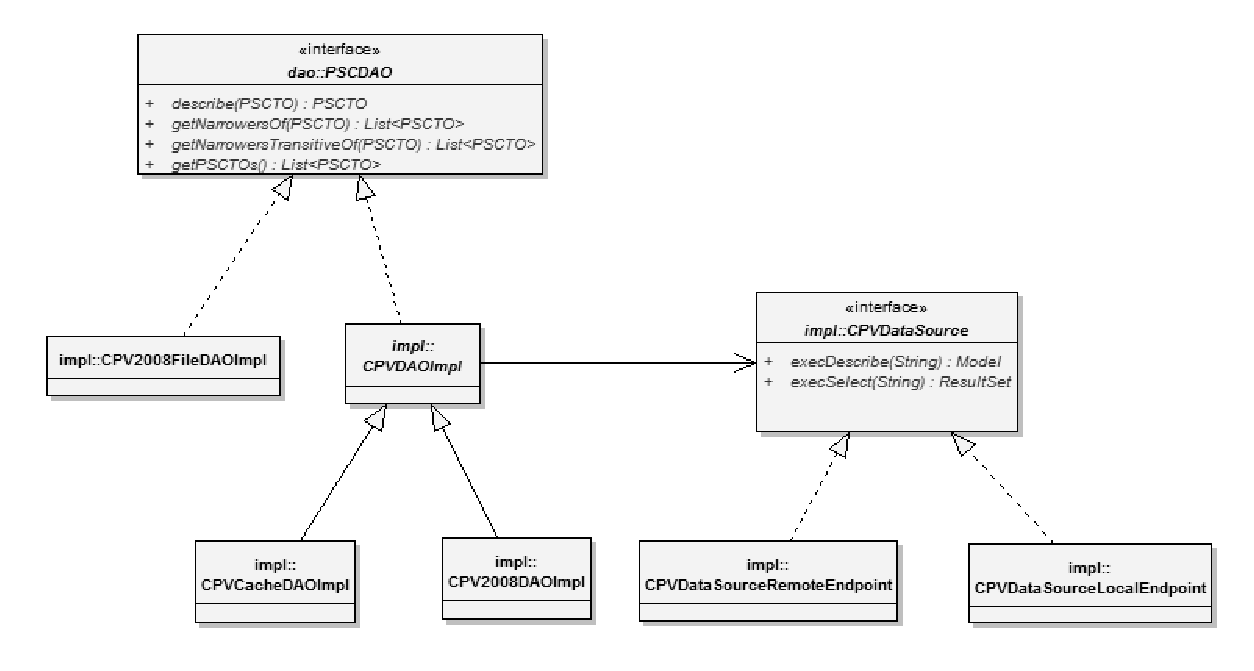
\includegraphics[width=16cm]{images/phd/moldeas/moldeas-dao}
\caption{Diagrama de Clases del acceso a datos (CPV) en \texttt{moldeas-api}.}
\label{fig:moldeas-api-dao}
\end{figure}


\item El paquete \texttt{appserv}, en el que se encuentran las clases con los servicios 
de negocio propios del sistema MOLDEAS, principalmente el servicio de recuperación 
de información y construcción de consultas en SPARQL a partir de un perfil de búsqueda 
del usuario. Adicionalmente, se encuentran clases relativas a la gestión de los objetos 
con la información de los anuncios de licitación.

\item  El paquete \texttt{enhancers}, en el que se establecen las interfaces para la 
expansión de las variables de información correspondientes a un perfil de búsqueda 
de anuncios de licitación. Entre los métodos especificados para realizar la expansión 
de consultas se encuentran aquellos relativos a \textit{Spreading Activation} a través 
de la biblioteca ONTOSPREAD~\cite{ontospreadWSKS11}, los basados en un motor de recomendación como Apache Mahout,
 los basados en un motor de búsqueda sintáctica como Apache Lucene y los relativos 
a las variables numéricas. 

\item El paquete \texttt{psc}, en el que se implementan las interfaces específicas relativas 
a la expansión de la variable de información de los anuncios de licitación correspondiente 
a los códigos de una clasificación de productos, en concreto del CPV 2008. Los métodos aquí 
utilizados son los relativos a la aplicación y configuración de las bibliotecas ONTOSPREAD, 
Apache Mahout, Lucene y Solr.

\item El paquete \texttt{standalone}, en el que se implementan las interfaces específicas 
para otras variables de información secundarias como la información geográfica o la cuantía 
del anuncio de licitación, en este caso de nuevo el principal componente utilizado es la biblioteca 
Apache Mahout configurada a través de distintos ficheros generados mediante el análisis 
del histórico de publicación de anuncios de licitación. Cada una de las implementaciones 
dependiendo de la información que se pretenda manejar debe tomar sus datos de una tabla 
previamente generada en el módulo de \texttt{moldeas-transformer}.

\item El paquete \texttt{ranking}, en el que se específica y se realiza una primera implementación 
de los operadores de agregación para establecer un orden los anuncios de licitación recuperados 
del \dataset RDF, ya sea través de un modelo en memoria o de un \textit{endpoint} de SPARQL. Para cada 
una de las variables de información presentes en los anuncios de licitación se establece una ponderación, cuando 
los anuncios de licitación son recuperados tras el proceso de expansión, se establece una puntuación 
mediante una función lineal que establece un valor según el anuncio extraído contenga más o menos 
elementos de los conjuntos relativos a los códigos \gls{CPV}, \gls{NUTS}, etc.

\item El paquete \texttt{business}, en el que se establece el interfaz de negocio para interactuar con los servicios 
del API, de esta manera se suministra un único punto de acceso como una caja negra, favoreciendo la 
abstracción del número de parámetros y las operaciones.
\end{itemize}

\begin{figure}[!htb]
\centering
	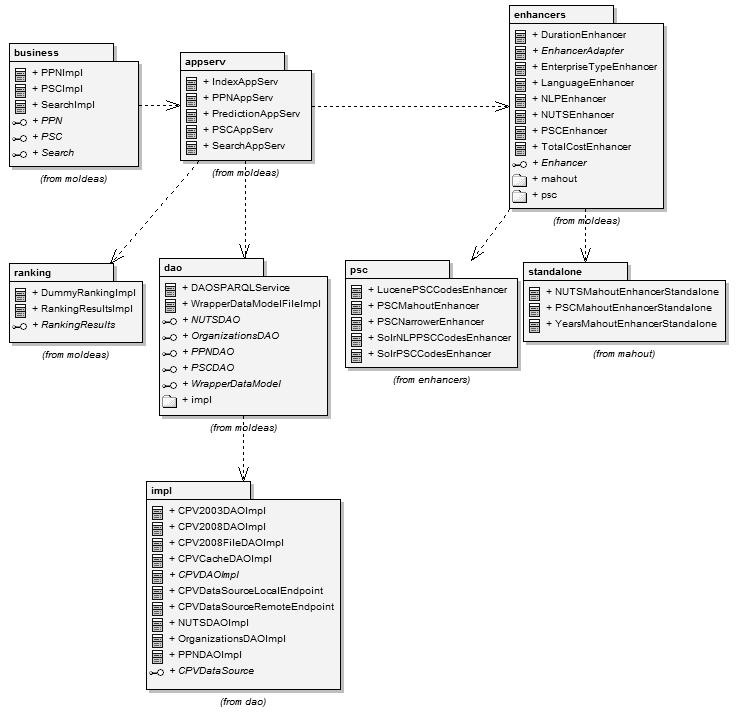
\includegraphics[width=16cm]{images/phd/moldeas/moldeas-api-packages}
\caption{Diagrama de Paquetes relevantes del componente \texttt{moldeas-api}.}
\label{fig:moldeas-api-packages}
\end{figure}

Una vez revisados los principales paquetes de \texttt{moldeas-api}, cabe realizar una descripción 
más completa del sistema de recuperación de información ya que el sistema de expansión de consultas 
se implementa a través de un patrón de diseño denominado \texttt{Chain of Responsibility} en el cual 
a través de distintas iteraciones y modificaciones de la consulta inicial se consigue un perfil 
enriquecido para ser traducido a una consulta en SPARQL. Evidentemente, el objeto contenedor 
del perfil de búsqueda de anuncios de licitación puede ser transformado a cualquier lenguaje de 
consulta tipo SQL o bien a una consulta de un motor de búsqueda sintáctica, esta abstracción 
se consigue de nuevo gracias a un uso correcto de interfaces. En primer lugar cabe especificar 
qué tipo de información y datos contiene un anuncio de licitación que como ya se ha repasado en 
el Capítulo~\ref{capitulo:metodos-separados} y concretamente en la Sección~\ref{sect:rdf-anuncios}, consta 
de una serie de variables de información conteniendo códigos del tipo de licitación, información geográfica, 
metainformación relativa a la cuantía del contrato, el perfil del contrante, la duración, etc. En general, 
y de acuerdo a la información disponible y su tipo se pueden establecer una serie de métodos para realizar la expansión 
de una consulta o perfil de búsqueda.

\begin{itemize}
 \item Información basada en conjuntos y modelada a través de una jerarquía, es el supuesto de los códigos CPV y de la información 
geográfica disponible en NUTS. En este caso los métodos que se pueden aplicar para expandir la consulta son los siguientes:
\begin{enumerate}
 \item Directo. Se navega a través de la jerarquía modelada buscando los elementos más específicos y estableciendo 
un peso determinado para cada uno de ellos. 
 \item Búsqueda Sintáctica. De acuerdo a las descripciones de los códigos se realiza una búsqueda en el \dataset correspondiente, 
buscando no sólo aquellos códigos que encajen perfectamente, sino también aquellos similares, mediante técnicas de procesamiento 
de lenguaje natural.
\item Motor de Recomendación. Realizando un procesamiento previo del histórico de anuncios de licitación y su información, se generan 
una serie de ficheros en los cuales se alinean los códigos CPV con la información relativa a la localización, cuantía o fecha, para que 
de acuerdo a una serie de códigos de entrada se genere una serie de información de salida.
\item \texttt{Spreading Activation}. En este caso se configura esta técnica para que tome un conjunto de conceptos de entrada, en general 
de códigos CPV, para obtener tras la ejecución del algoritmo un conjunto de salida ponderado.
\end{enumerate}

\item Información numérica o asimilable. Se trata el caso de la duración del contrato, la cuantía del mismo, 
el radio de acción geográfico, etc. En este caso los métodos que se pueden aplicar para expandir la consulta son los siguientes:
\begin{enumerate}
\item Basado en el usuario. El perfil de búsqueda del propio usuario define los rangos en los cuales se debe hallar una variable 
numérica sin necesidad de realizar ningún proceso de expansión automático.
\item Uso de lógica borrosa. Se ha valorado el uso de estas técnicas para establecer un intervalo en el cual ponderar 
la pertenencia de un valor a un conjunto. No obstante, en esta primera versión del demostrador público estas técnicas implementadas 
a través de la biblioteca \textit{JFuzzyLogic} tan sólo se han probado y no se han introducido como parte del proceso de 
búsqueda.
\end{enumerate}

\end{itemize}

El objetivo final de estos métodos es obtener para cada una de las variables de información de un perfil 
de anuncio de licitación, una puntuación que permite ejecutar un operador de agregación para así establecer 
un orden entre los anuncios de licitación extraídos tras la generación de la consulta. La importancia de este 
procedimiento por fases reside en que cada uno de los pasos y métodos de expansión se modelan mediante interfaces y 
son ejecutados mediante un proceso iterativo de enriquecimiento, como se puede ver en la Figura~\ref{fig:moldeas-api-search}, 
que permite la adición de nuevos métodos de forma sencilla, simplemente reconfigurando las implementaciones de 
los interfaces a través del fichero de configuración de Spring. El flujo y la comunicación 
entre las distintas clases que intervienen en el proceso de expansión y recuperación de información 
se presenta a través de la Figura~\ref{fig:moldeas-search}, en el cual es preciso señalar 
como las responsabilidades son compartidas a través de los distintos objetos situados en distintas 
capas lógicas.

\begin{figure}[!htb]
\centering
	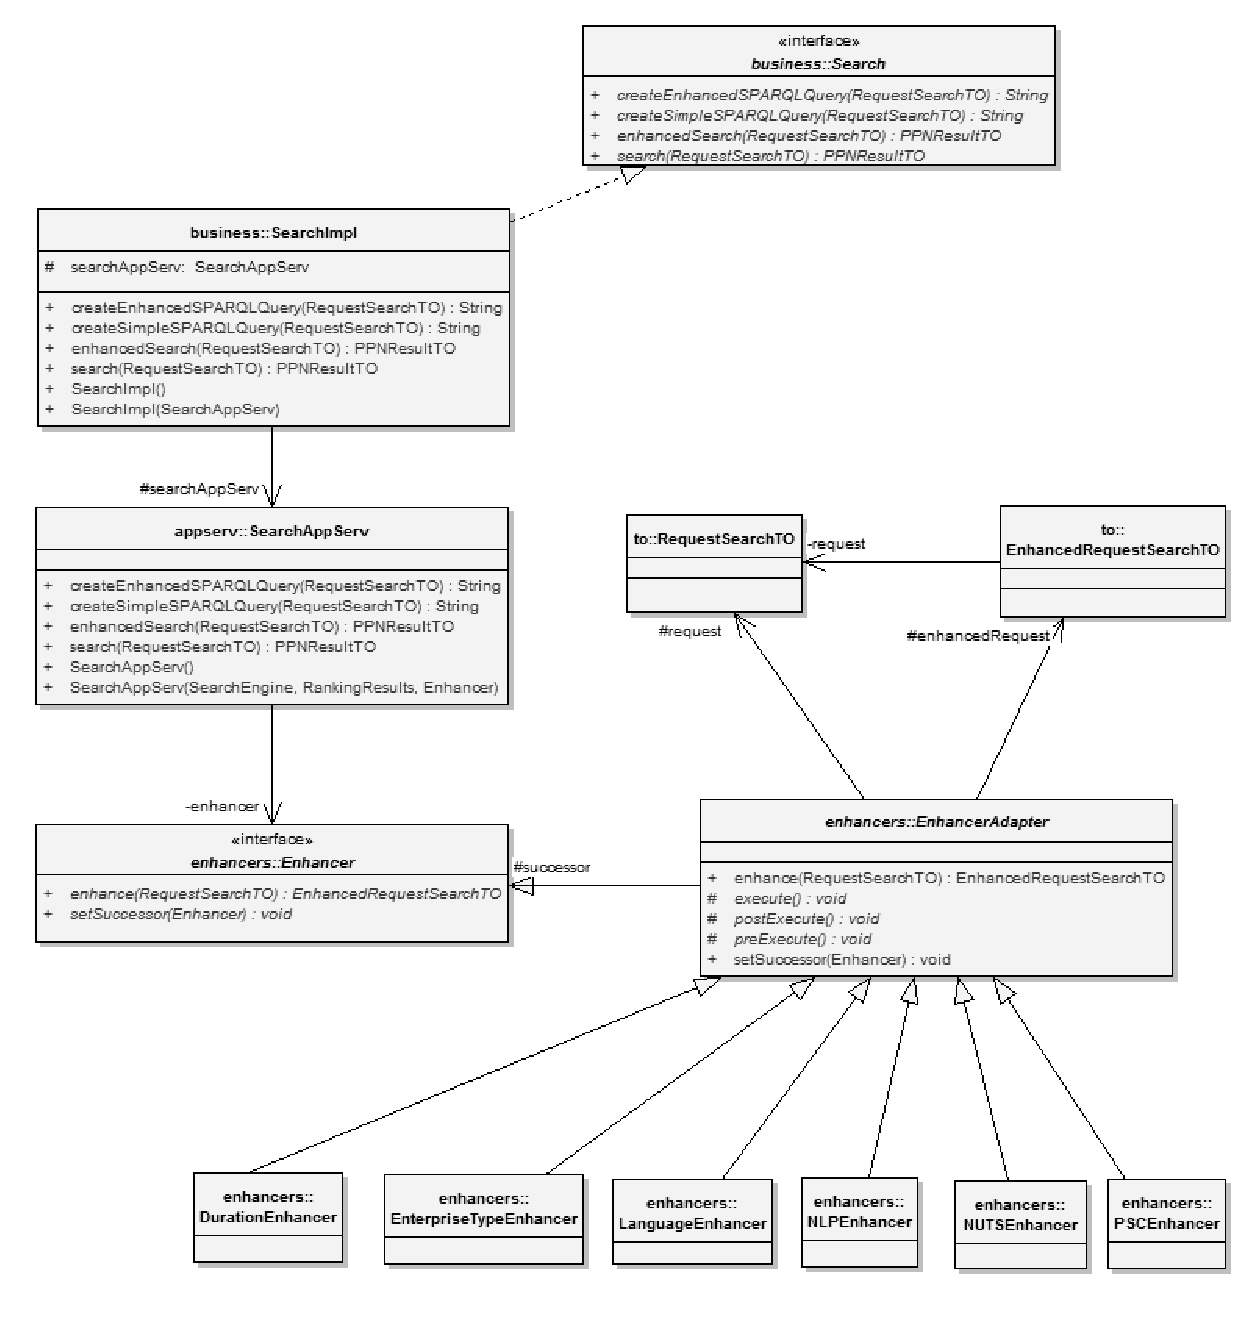
\includegraphics[width=16cm]{images/phd/moldeas/moldeas-chain}
\caption{Diagrama de Clases del sistema de búsqueda en \texttt{moldeas-api}.}
\label{fig:moldeas-api-search}
\end{figure}


\begin{figure}[!htb]
\centering
	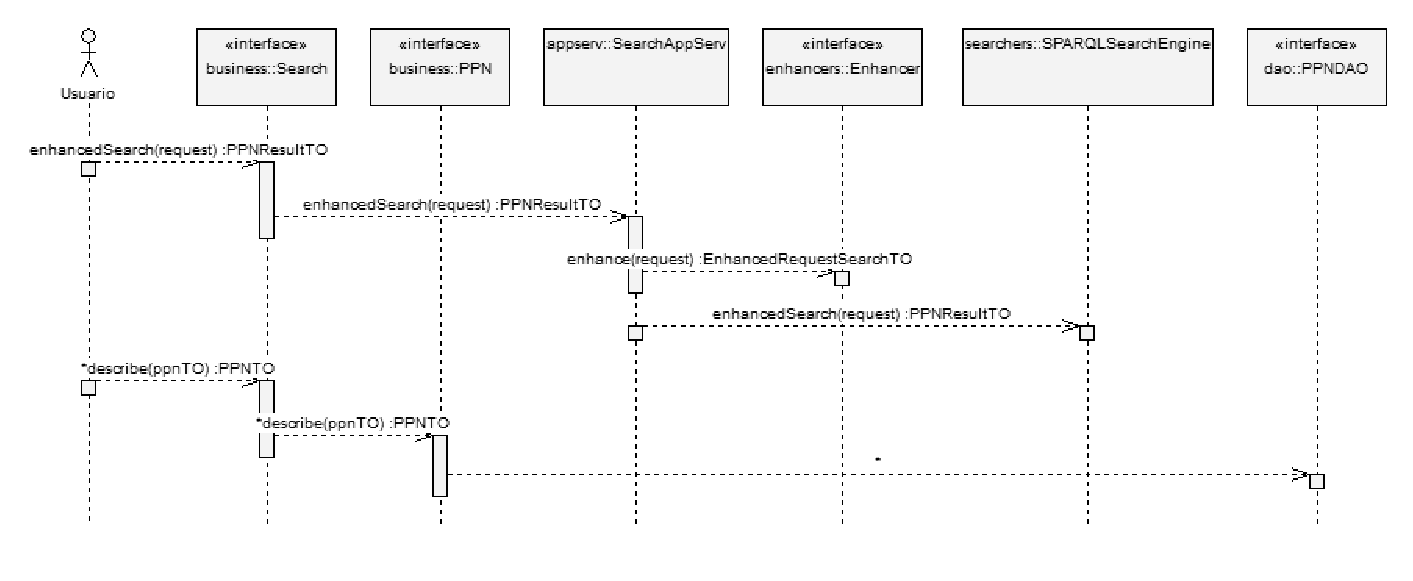
\includegraphics[width=16cm]{images/phd/moldeas/moldeas-search}
\caption{Diagrama de Secuencia de la búsqueda en \texttt{moldeas-api}.}
\label{fig:moldeas-search}
\end{figure}


Finalmente, en este apartado cabe señalar los patrones de diseño, ver Tabla~\ref{tabla:patrones}, que se han aplicado 
para obtener un sistema flexible y escalable en el cual nuevas implementaciones 
de los interfaces sean fácilmente integrables proporcionando un API para el consumo de datos enlazados y recuperación de información de los anuncios de 
licitación.


\begin{table}[htb]
\renewcommand{\arraystretch}{1.3}
\begin{center}
\begin{tabular}{|p{6cm}|p{8cm}|}
\hline
        \multicolumn{2}{|c|}{\textbf{Patrones de Diseño}}\\        
        \hline
        \textbf{Nombre} &  \textbf{Aplicación} \\ \hline       
			\textit{Adapter}&Implementación para el acceso y transformación de los datos de los anuncios de licitación.\\ \hline
			\textit{Chain of Responsibility}&Implantación del sistema de enriquecimiento de consultas.\\ \hline
			\textit{DAO}&Abstracción de acceso a la base de datos y de conocimiento.\\ \hline
			\textit{Template Method}& Implementación por omisión de métodos en el patrón \textit{Chain of Responsibility}.\\ \hline
			\textit{Factory Method}&Creación de objetos provenientes de Spring.\\ \hline
			\textit{Template Method}&Funciones con llamadas a métodos de interfaces, por ejemplo en los \texttt{Enhancers}.\\ \hline
			\textit{Transfer Object}&Comunicación de información entre los distintos módulos y capas.\\\hline 
			\textit{Singleton}&Creación de objetos de acceso a datos, etc., provenientes de Spring.\\ \hline
			\textit{Otros}&Relativos al diseño por capas de aplicaciones J2EE.\\ \hline
		\hline
		\end{tabular}
		\caption{Principales Patrones de Diseño utilizados en MOLDEAS.}
		\label{tabla:patrones}
  \end{center}
\end{table} 

\clearpage
\subsection{Diseño de \texttt{moldeas-test}}\label{sect:moldeas-test}
El objetivo de este módulo es abstraer las pruebas de los módulos anteriores, 
especialmente de \texttt{moldeas-api}, para así proveer un sistema separado 
de ejecución de \textit{tests} en el cual se puedan realizar las siguientes 
acciones:

\begin{itemize}
 \item Creación de configuraciones del \gls{API} de \gls{MOLDEAS} a través de distintos 
ficheros de Spring que permiten probar de forma automática la combinación 
de los distintos métodos de expansión de consultas así como verificar 
sus resultados.
\item Validación de los recursos \gls{RDF} generados de acuerdo a unas reglas de validación 
extraídas de las tablas de validación establecidas en el Apéndice~\ref{tablas-validacion-apen}.
\end{itemize}

De esta manera se ofrece un módulo separado con un doble sentido, para la realización de pruebas de caja negra de los 
servicios disponibles en el API de MOLDEAS, así como para la propia validación de los datos enlazados. La configuración 
de este módulo se realiza a través de un fichero \gls{XML} \textit{ad-hoc} en el cual se cargan las configuraciones 
para ejecutar los \textit{tests} pertinentes (en forma de plantilla) mediante Junit. No obstante, en la Sección~\ref{sect:pruebas-moldeas} se realiza una descripción 
más detallada de las pruebas llevadas a cabo.


\subsection{Diseño de \texttt{moldeas-web}}\label{sect:moldeas-web}
El objetivo principal de diseño de este módulo es definir y diseñar un herramienta de acceso gráfico 
a los servicios del sistema \gls{MOLDEAS}. Es importante destacar que este cliente gráfico se realiza con el objetivo de facilitar 
un demostrador público ya que el uso de la biblioteca de \texttt{moldeas-api} es perfectamente 
válido desde cualquier programa así como desde el interfaz de servicios REST, que también se incluye 
en este módulo. Por tanto, este módulo surge para abarcar las siguientes funcionalidades:

\begin{enumerate}
\item Proveer un interfaz de servicios \gls{REST} que sirva tanto para exponer los 
servicios de negocio, como para ejemplificar las llamadas del \gls{API} de MOLDEAS.

El interfaz de servicios REST diseñado, simplemente añade una capa extra de indirección a los 
servicios de negocio suministrados en el API de MOLDEAS, se duplica la signatura de los métodos 
en una nueva capa simplificando las llamadas. La idea de realizar un interfaz REST surge para dar soporte a la tendencia actual de publicación 
de servicios web \gls{HTTP} y también para ejemplificar las llamadas al API (construcción de parámetros, gestión 
de los resultados, etc.), en cualquier caso, cualquier cliente siempre puede utilizar 
la versión de \texttt{moldeas-api} empaquetada individualmente. Para realizar este API de servicios 
REST se ha utilizado la biblioteca para Java-Jersey \gls{REST} 0.8 y la descripción de los mismos 
se presenta, parcialmente, en la Figura~\ref{fig:moldeas-wadl} en formato \gls{WADL}.


\begin{figure}[!htp]
\lstinputlisting[language=XML,basicstyle=\scriptsize]{examples/moldeas-pretty.wadl}
	\caption{Interfaz REST en formato WADL.}
	\label{fig:moldeas-wadl}
\end{figure}


\item Suministrar un interfaz gráfico que ejemplifique las llamadas a los servicios REST y que a su vez sirva como demostrador público para el acceso a los datos de los anuncios de licitación 
y para la recuperación de información. La construcción de este interfaz se ha desarrollado utilizando 
bibliotecas de Jquery y HTML facilitando la creación de interfaces enriquecidos de programación 
sencilla.

\item Aunar las herramientas externas de publicación y acceso a datos enlazados en un sólo punto de entrada. En este sentido, 
el interfaz web creado también contempla ejemplos de consultas en SPARQL a realizar mediante la herramienta 
\gls{SNORQL} y enlaces a ejemplos de recursos que son consultados a través de un \linkeddata \textit{front-end} como 
Pubby.
\end{enumerate}

\subsubsection{Conceptos y Diseño de la Interacción Gráfica}
En los últimos años, el aumento en el uso de las nuevas tecnologías de la información ha 
conllevado un cambio fundamental en la sociedad que provoca la necesidad de adecuarse a nuevas 
relaciones que se establecen entre la persona y la máquina. Esta necesidad de interacción supone 
que la comunicación entre persona y máquina adquiera una especial relevancia en nuestro tiempo. Se maniesta
 un desafío consistente en proporcionar de significado a los productos y servicios ofrecidos, 
intentando dotarlos de estructura y comprensión cercana a la escala humana.

Debido a la complejidad interna de los ordenadores, la comunicación entre los entes debe realizarse 
a un nivel conceptual, predominando la comunicación visual, gráfica y verbal como medio para llegar 
a la comprensión. La idea subyacente está referida a la necesidad de encontrar el modelo ideal que permita a la persona 
interaccionar con las máquinas como si fueran un humano más.

En esta situación se hace especialmente relevante la generación de interfaces de usuario 
que se adecúen a las necesidades de las personas, por ello las reglas propuestas por 
\textit{Sneiderman} suponen un primer acercamiento a la interacción persona ordenador y una 
métrica para evaluar la bondad de un interfaz de usuario.

En este sentido, desde los anales de la historia los hombres han ideado formas e instrumentos
(lenguajes de símbolos, de texto, gráficos, etc.), tanto para la comunicación de sus experiencias, 
como para reproducir la realidad. La forma de expresión depende en buena medida del ambiente 
tecnológico y de los lenguajes utilizados entre el emisor y el intérprete para decodificar los mensajes. 

La riqueza de expresión de un lenguaje se basa en el principio de concordancia entre los entes 
participantes del acto comunicativo, para que se establezca este acto deben estar en correcta relación. 
Desde el punto de vista de un interfaz gráfico estos factores quedan patentes por la dificultad 
que entraña ofrecer un entorno en el cual tanto: percepción, interpretación y comprensión sean 
lo suficientemente claros para que el ser humano no se sienta en un entorno extraño.

Los seres humanos a través de su sistema nervioso son capaces de percibir 
lo que sucede en su entorno y actuar en consecuencia, puede considerarse que el hombre es una fuente de información, percibe 
y recibe estímulos externos que le permiten adaptar sus respuestas. 

Comprender el comportamiento humano como sistema de comunicación supone una gran dificultad, 
tanto en capacidad para interpretar, como para decodificar los mensajes, haciendo imposible 
conocer su respuesta exacta ante la recepción de un mensaje. El problema de la comunicación entre personas y 
máquinas no consiste en reducir el comportamiento humano al de una máquina, sino analizar 
las necesidades y capacidades para adaptar la presentación de información a su nivel, acercándose 
lo más posible al proceso cognitivo de la persona.

La visión es nuestro medio natural de percepción de los mensajes, limitada por condiciones físicas, 
por ello cobra especial relevancia para la distribución de información en un documento, 
dependiendo la compresión de la persona de la bondad de la misma. No obstante, este modelo a seguir no es 
completamente válido ya que habría que tener en cuenta las necesidades de las personas con discapacidades de distinto tipo, 
intentado adaptar el contenido al sujeto participante de la comunicación.

Utilizando los distintos sentidos de los que disponemos como fuentes de adquisición de información 
debemos ser capaces de procesar y comprender esta información, esta capacidad puede denominarse 
\textit{entendimiento humano}, mediante el que determinamos nuestros actos a partir de las percepciones 
sensoriales. De todos los estímulos percibidos, sólo permanecen aquellos que generan un mayor impacto, 
este será un factor muy relevante en el diseño de un interfaz, por ejemplo cuando se selecciona una combinación de colores.

Debe tenerse en cuenta, que aunque el funcionamiento general humano es similar no puede ser 
predecible, ni aplicable por extensión, se cometería en un grave error de 
interpretación del comportamiento, este punto es especialmente interesante a la hora de adaptar un interfaz 
gráfico a las distintas personas, estableciendo perfiles.

Las 8 reglas de Oro de \textit{Sneiderman} nos ayudan a este objetivo, intentando simplificar 
la comunicación persona-máquina. A continuación, se comentan estas reglas:

\begin{description}
\item[Esforzarse por la consistencia.] Es el principio por el cual los
elementos y relaciones deben ser presentados de forma idéntica e inequívocamente. Este concepto es aplicable a:
\begin{itemize}
\item Tipografía, por ejemplo enfatizar siempre con el mismo estilo.
\item Iconos, la misma acción debe estar representada por el mismo icono.
\item Comandos y menús, la información que se utilice en los menús deberá ser representativa
de su acción interna.
\item Funcionamiento multiplataforma, esta cualidad se pone de manifiesto actualmente, ya que se accede a la misma información utilizando diferentes medios: navegadores, móviles, etc.
\item Percepción del sistema igual para todos los usuarios.
\item Estructura el sistema de forma que se adapten al entorno de trabajo del usuario.
\end{itemize}

Por lo tanto la consistencia nos remite a obtener una representación de los objetos 
coherente en su significado, formas y métodos en el mismo contexto. 
También puede entenderse la consistencia como la relación que se establece entre 
una metáfora de representación y su uso real.

\item[Permitir a los usuarios frecuentes utilizar atajos:] se considera un
usuario frecuente a una persona que interacciona con un interfaz gráfico con soltura, debido 
sobre todo a la experiencia en su uso. Este tipo de usuarios, a medida que avanza su 
manejo del interfaz, se convierten en expertos, exigiendo mayores prestaciones a la aplicación desde distintos puntos de vista: 
1) adaptabilidad y 2) velocidad de ejecución.

Esta característica a tener en cuenta en los interfaces, se aplica no sólo a los usuarios 
expertos sino a la necesidad de que un interfaz sea adaptable a las nuevas necesidades que se 
manifiestan en el usuario a través del uso.

Por otro lado, los atajos deben ser fáciles de recordar y mejorar el rendimiento, por ejemplo 
sería contraproducente un atajo de teclado de cuatro teclas ya que sólo el posicionamiento correcto 
de los dedos sería más penalizador que utilizar un ratón.

\item[Ofrecer retroalimentación informativa.] Debido al concepto de acto
comunicativo, resulta importante que cuando un usuario realiza una acción se vea recompensada con una respuesta del sistema. 
De esta forma, se consigue que se establezca la metáfora de la comunicación entre el 
emisor (usuario) y el receptor (máquina), permitiendo una comunicación fluida.

Este objetivo es relevante en cuestiones relacionadas con el establecimiento del éxito o no de la operación 
realizada por el usuario, por ejemplo si en un navegador no se dispone de conexión a internet 
y se solicita el acceso a una página, el proceso de espera sería tedioso, utilizando una barra de 
progreso de carga se consigue realimentar el estado de la acción solicitada e iniciada por el usuario.

\item[Diseñar diálogos para fundamentar el cierre.] Con esta característica
se consigue acotar el inicio de una secuencia de acciones, fijando
su inicio, desarrollo y final. Respetando este punto se consigue que el usuario se sienta satisfecho, ya que sabe si la acción que ha realizado ha seguido la secuencia correcta, utilizando todos los pasos previstos hasta llegar a un fin.

\item[Ofrecer prevención de errores y manejo de errores simples.] La gestión de
errores es importante en cualquiera de los aspectos dentro de una aplicación informática.
En el contexto de un interfaz de usuario queda patente la necesidad y las ventajas que conlleva 
disponer de un interfaz que minimice los errores, involuntarios o no, provocados por los usuarios.

Un escenario de uso podría ser la introducción de una fecha, generalmente para facilitar 
la interacción con el usuario se genera una máscara de entrada o bien un ejemplo que 
permita al usuario cambiarlo para así facilitar sus tareas.

El objetivo, es que el usuario se preocupe de sus tareas y no del funcionamiento del 
interfaz, es decir, que el manejo del mismo no suponga un trabajo extra.

No obstante, este objetivo no siempre se puede conseguir, de ahí que cuando se produzcan errores 
no críticos de la aplicación, tales como errores en la introducción de 
datos o una secuencia de pasos inválidos para realizar una acción, sería conveniente que el sistema fuera capaz de ofrecer 
un mecanismo tutor para enseñar al usuario al manejo sin errores. 
Un claro ejemplo podría ser el famoso ``ayudante'' de Microsoft Word que si bien realiza su función, en ocasiones llega a resultar molesto.

Los tutores dentro de las aplicaciones para aleccionar a los usuarios, y prevenir errores, 
se deben diseñar con sumo cuidado y acotando muy bien su ámbito de acción ya 
que su efecto puede ser el contrario del pretendido. En estos casos, el menos es más puede 
resultar útil y un simple texto desplegable con un ejemplo puede ser suficiente.


\item[Permitir inversión de las acciones.] Esta característica ofrece la
admirable ventaja de ofrecer confianza al usuario en su diálogo con el interfaz gráfico. 
Suponiendo que un usuario novel realiza una serie de acciones secuenciales y antes de grabar 
los cambios se percata de que ha cometido un fallo, podría pensar en distintos escenarios, así:
\begin{itemize}
\item Tranquilidad, el interfaz permite deshacer cambios, se puede retroceder para corregir lo que se ha realizado de forma incorrecta.
\item Desconsuelo, después de estar X tiempo realizando una tarea se tiene que deshacer debido a un insignificante error, tiempo perdido.
\end{itemize}

Parece claro que el sentimiento de tranquilidad es más deseable en un usuario, así que es 
importante cumplir esta característica.

Desde otro punto de vista, el usuario se sentirá más tranquilo y seguro en el uso del interfaz 
si sabe que tiene más de una oportunidad cuando utiliza las funciones de la aplicación, 
de otra forma un sentimiento de angustia podría invadirle produciendo errores en el usuario y 
empeorando su rendimiento en el uso de la aplicación.

El sentido de estos cambios debería ser tanto hacia adelante como hacia atrás, ya que sino se desaprovecha 
la potencia de esta propiedad.

\item[Apoyar el control de los usuarios:] en la tarea de satisfacer al usuario,
éste debe percibir que el sistema está ejecutándose bajo su supervisión y respondiendo a sus acciones. 
Todo aquello que sea público al usuario deberá permitir su control, siempre dentro de unos límites, 
ya que de otra forma quizás se obtuviera un sentimiento de insatisfacción.

Debería evitarse por ejemplo introducción de datos tediosa, comportamiento extraño de la aplicación 
(acciones o comandos que no funcionan o no responden) o imposibilidad de obtener información 
(sabemos que se ha introducido pero se desconoce cómo acceder a ello).

\item[Reducir la carga de la memoria a corto plazo:] esta necesidad surge por
una limitación en la memoria humana para procesar información a corto plazo, por ello, cuando 
un interfaz emita mensajes al usuario deberán ser cortos de modo que pueda comprender 
rápidamente la información que se envía desde la máquina.

También es conveniente no tener demasiadas ventanas abiertas dentro de un entorno, 
ya que pueden despistar al usuario y no saber dónde está exactamente.

\end{description}

El diseño de un interfaz gráfico para el sistema MOLDEAS es una tarea relativamente
sencilla, ya que el problema real consiste en suministrar un interfaz habitual 
al usuario en el cual pueda seleccionar las características de su perfil 
de búsqueda. En cualquier caso, se optado por un interfaz gráfico 
lo más sencillo, intuitivo, consistente y uniforme posible.









\section{Pruebas del Sistema MOLDEAS}\label{sect:pruebas-moldeas}
La metodología de la Programación Extrema~\cite{XP} (\gls{XP}), que ha servido de guía para el desarrollo 
del sistema MOLDEAS, hace hincapié en la importancia de las pruebas. La realización de ciclos de desarrollo breves
(incorporando la funcionalidad perseguida en pequeñas versiones totalmente funcionales) habilita la posibilidad de 
concentrarse en la validación, en cada momento, de un segmento reducido del código o de la funcionalidad, 
dependiendo del nivel de la prueba. Pero también exige la existencia de un mecanismo que permita 
realizar los ensayos de forma automática; de lo contrario, la obligación de repetirlos 
frecuentemente los convertiría en extremadamente tediosos.

\subsection{Pruebas Caja Blanca}
Son pruebas que se realizan para verificar la validez de las operaciones internas del programa, 
intentando garantizar que todos los caminos de ejecución del programa han sido probados. Para realizar las pruebas de caja blanca se han 
seleccionado las pruebas unitarias por su importancia dentro la metodología de Programación Extrema. 
La descripción de las pruebas unitarias se amplia a través de los siguientes puntos.

\begin{description}

\item [Validación con pruebas unitarias:] representan el nivel más bajo de prueba del \textit{software}, 
permitiendo al desarrollador obtener retroalimentación instántanea del correcto
comportamiento (o no) de un componente determinado.

\item [Necesidad de las pruebas unitarias:] como buena práctica de programación
el desarrollador debería codificar la prueba antes que la propia funcionalidad,
para así pensar los resultados antes de obtenerlos. Como norma general, un buen
test siempre debería fallar la primera vez. Por otra parte, facilitan la
depuración, si un test falla tenemos un ámbito muy reducido en el cual localizar
el error, se incrementa la productividad de los desarrolladores. 

Además, desde el punto de vista de la gestión de un proyecto un buen conjunto de
pruebas unitarias se pueden utilizar como documentación del código fuente, así,
por ejemplo si se introducen nuevos desarrolladores éstos pueden comprender
fácilmente la funcionalidad que se está realizando y probando.

\item [Codificación de Pruebas:] las pruebas unitarias deben seguir una serie de
criterios:
\begin{itemize}
  \item Prueban funcionalidad determinada, un método.
  \item Ejecución rápida, si no fuera así los test sólo se ejecutarían
  cada cierto tiempo repercutiendo en la integración del código.
  \item Se debe determinar sobre qué clases se van a generar casos de prueba. No
  todas las clases y métodos son candidatos a ser probados.
  \item Son independientes de otras pruebas.
  \item Deben ser independientes de terceros, por ejemplo de una base de datos.
\end{itemize}

\item [\textit{Refactoring}:] despues de que una componente haya pasado un test unitario,
ya podemos aplicar las técnicas de \textit{refactoring} para mejorar la calidad
de código. Este proceso conjunto de prueba y recodificación, lo podemos realizar
ya que tenemos una manera de probar la funcionalidad de forma automática. En las
primeras etapas de desarrollo será cuando se haga más intenso el uso de pruebas
unitarias ya que estaremos codificando nueva funcionalidad en cada momento.
\end{description}

\subsubsection{Junit}\label{junit}
Herramienta Java para la realización de pruebas unitarias de
programas, ejecuta test de pruebas de forma automática realizando un registro de
los resultados obtenidos. El gran éxito de esta herramienta se debe a su
facilidad de uso en comparación con el trabajo que realiza.

La realización de las pruebas de los programas normalmente resultan costosas
temporalmente y muchas veces no se almacenan ni se documentan. Con esta
herramienta, se consigue que la prueba de programas rebaje su coste, además de
liberarnos de una parte de la construcción de programas que en muchos casos
resulta pesada y poco eficiente.

Por todo esto, con Junit se aumenta el nivel de calidad en el test de los programas,
entendiendo por calidad en el test como una mejora en la realización de
las pruebas en cuanto a casos contemplados, número y registro de las mismas y facilidad de uso.

Las ventajas de uso de Junit se pueden resumir en los siguientes puntos:
\begin{itemize}
\item Facilidad de uso.
\item  Creación de conjuntos de pruebas para una clase.
\item  Combinación con otras herramientas de gestión de proyectos como Maven.
\item  Código libre.
\item  Bien documentado.
\item  Pruebas a diferentes niveles y capas.
\item  Extensible.
\end{itemize}

Cabe señalar que existen extensiones de Junit que permiten realizar pruebas en
distintos ámbitos, siempre y cuando hayamos seguido un diseño apropiado. 
De esta manera existen \textit{frameworks} basados en Junit para probar:
\begin{itemize}
\item  XmlUnit, para documentos XML.
\item  DbUnit, para probar el estado de la base de datos.
\item  EasyMock, para generar las clases que basadas en nuestras interfaces de
negocio nos permitan probar los servicios y funcionalidad de la aplicación.
\item  HttpUnit, JWebUnit o Cactus para las distintas capas de
una arquitectura cliente/servidor.
\end{itemize}

El contexto del sistema \gls{MOLDEAS} se han realizado $140$ \textit{tests} enclavados 
dentro de $48$ clases Java específicas para Junit.

\subsection{Pruebas de Caja Negra}
Son pruebas que se centran en los requisitos funcionales del
\textit{software}. Existen diferentes tipos como: prueba de los valores
límites o partición equivalente. Para realizar este tipo de pruebas se utilizan
posibles entradas al sistema y se verifica que cumple con los resultados
esperados. Las pruebas realizadas para la validación del sistema de recuperación 
de anuncios de licitación se pueden considerar dentro de este tipo de pruebas de caja negra y teniendo en cuenta
que el sistema \gls{MOLDEAS} trabaja con una configuración externa, su funcionamiento
dependerá de la misma y no del programa en sí, es decir, desde un punto de vista
de software la implementación realizada representa un conjunto de 
configuraciones a través de Spring. Considerando el carácter investigador 
de este estudio, resultan más relevantes las pruebas de
validación científica que las propias de caja negra, más apropiadas 
desde un punto de vista de aplicación de \textit{software}.


\subsection{Aportaciones Finales sobre las pruebas}
La codificación de pruebas unitarias antes de codificar cierta funcionalidad
puede resultar tediosa e incluso considerarse un retraso en el desarrollo, pero
no es así, ya que el disponer de método eficaz para realizar pruebas ayuda en
posteriores etapas a la codificación de determinada función y asegura una cierta
calidad en el \textit{software}. 

Por ejemplo, se realiza un determinado método para una cierta tarea. Para realizar la prueba se utiliza 
un método \textit{main} en la propia clase donde se ha definido y una vez que se comprueba que todo
funciona correctamente ese método \textit{main} se elimina, otorgando a esa
funcionalidad la etiqueta de éxito. Un tiempo más tarde, nuevsa situaciones obligan a 
modificar el código de esa clase porque no se habían contemplado todos los
requisitos funcionales, pero, ¿quién se atreve a recodificar esa función?, ¿cuál era su comportamiento?, 
¿para qué utilizaba esa variable? y ¿cómo se prueba que mantiene su funcionalidad anterior (necesario para otros módulos) y 
que además incorpora la nueva funcionalidad?. La respuesta es sencilla, se volverá a codificar un método
\textit{main}, se crea un nuevo caso prueba y practicamente se delega en la ``suerte'' que entregue 
un comportamiento correcto tanto para la versión anterior como para las nuevas funcionalidades. En 
conclusión, una prueba unitaria hubiera facilitado el desarrollo, ya que tan sólo se debería generar un
caso de prueba para la nueva funcionalidad. Pero en cambio, se ha perdido tiempo: codificando métodos que 
para luego ser eliminados, pensando en qué hacía la función, para qué se utiliza cierta variable, etc. 

En definitiva, las pruebas unitarias facilitan el desarrollo de \textit{software} de
calidad, en contraposición de los engendros (no desarrollos) de \textit{software} creados
al margen de la realización de pruebas.

\subsection{Métricas de código fuente}
La calidad del \textit{software}, en cuanto a código fuente, es uno de los requisitos que se
debe exigir a cualquier aplicación. Normalmente, no se plantea como uno de los
requisitos no funcionales prioritarios y esto provoca que aunque se haya
realizado un buen análisis e incluso un buen diseño, el código generado no es lo suficientemente bueno y es el
origen de todos los posibles errores y en consecuencia no se cumple con los
requisitos funcionales establecidos. La definición de calidad de \textit{software}, de
forma genérica, es mucho más extensa:  

\begin{definition}
Concordancia con los requisitos funcionales y de
rendimiento explícitamente establecidos con los estándares de desarrollo
explícitamente documentados y con las características implícitas
que se espera de todo \textit{software} desarrollado profesionalmente. R.S. Pressman (1992).
\end{definition}

\begin{definition}
El conjunto de características de una entidad que le confieren su
aptitud para satisfacer las necesidades expresadas y las implícitas. \gls{ISO} 8402
(\gls{UNE} 66-001-92).
\end{definition}

Estas definiciones de calidad se refieren sobre todo a la metodología utilizada y
al grado de satisfacción de los requisitos funcionales del producto \textit{software}. 

Las métricas que aquí se presentan constituyen medidas de calidad del código fuente, ya
que se estima que los requisitos funcionales han sido cubiertos al obtener un
prototipo experimental que ha sido probado a través de distintos conjuntos de pruebas.

A continuación, se presentan una serie de métricas de calidad de código fuente
(sólo del componente \textit{moldes-api}), obtenidas mediante el \textit{plugin} Metrics de Eclipse, que 
permite generar una serie de medidas, ver Tabla \ref{tabla:metricas}, significativas del código fuente, basadas en 
las definiciones realizadas en el libro \textit{Object-Oriented Metrics, measures of Complexity} de Brian Henderson-Sellers, Prentice Hall, 1996. 

Estas métricas miden, principalmente, valores de cohesión y acoplamiento que nos permiten establecer si el código está bien estructurado. 
Sin entrar en detalles precisos de los tipos y niveles de cohesión y acoplamiento, estas dos características se pueden definir como:

\begin{definition}
Cohesión, consecuencia del ocultamiento de la información. Un módulo con
cohesión (Pressman en ``Ingeniería del Software: Un enfoque práctico'')
realiza solamente una tarea, requiriendo poca
interacción con el resto de los procedimientos que se realizan en el resto del
sistema de \textit{software}. 
\end{definition}

Según \textit{Sommerville} en ``Requirements Engineering. Processes and Techniques'' la cohesión es deseable
debido a que una unidad (componente) representa una parte
simple de solución. Si es necesario cambiar el sistema, la parte
correspondiente está en un solo lugar y lo que se desee hacer con
él estará encapsulado en él. La meta, según
\textit{Lawrence} en ``Ingeniería del \textit{software}: Teoría y práctica'', es hacer que los componentes sean lo más cohesivos posible.


\begin{definition}
Acoplamiento, está relacionado con la cohesión. Es un
indicador de la fuerza de interconexión entre los componentes o
elementos de la arquitectura 
\end{definition}

Los sistemas altamente acoplados tienen una fuerte interconexión, lo que se
refleja en una gran dependencia entre los componentes. Los
sistemas poco acoplados, por otro lado, tienen poca relación entre
sus componentes o elementos. El objetivo, según (\textit{Lawrence}), es mantener el
acoplamiento en el nivel más bajo posible; la conectividad sencilla entre
módulos da como resultado un \textit{software} que es más fácil de comprender y menos
propenso al ``efecto onda'' producido cuando los errores aparecen en una
posición y se propagan a lo largo del sistema. 


   \begin{longtable}{|p{2cm}|p{3cm}|p{8cm}|}

      \hline 
	    \multicolumn{3}{|c|}{\textbf{Métricas de código fuente}}\\ \hline
	     \textbf{Tipo} &  \textbf{Descripción (EN)} &  \textbf{Descripción (ES)} \\ \hline
      \endhead
			NSM&\textit{Number of Static Methods} & Número total de métodos estáticos.\\ \hline
			TLOC&\textit{Total Lines of Code}&Número total de líneas de código. No incluye
			comentarios ni líneas en blanco.\\ \hline 
			CA&\textit{Afferent Coupling} &Número de clases fuera del paquete que dependen de
			clases dentro del paquete.\\ \hline 
			RMD&\textit{Normalized Distance} & $|RMA + RMI - 1 |$, este número debe ser pequeño.
			Cercano a 0 indica un buen diseño de paquetes.\\ \hline
			NOC&\textit{Number of Classes}& Número total de clases.\\ \hline
			SIX&S\textit{pecialization Index} &Indice de especialización :$NORM * DIT / NOM$\\			\hline 
			RMI&\textit{Instability} & $CE / (CA + CE)$\\ \hline
			NOF&\textit{Number of Atributtes} &Número de atributos definidos en un ámbito.\\ \hline
			NOP&\textit{Number of Package}s& Número  total de paquetes\\ \hline
			MLOC&\textit{Method Lines of Code} & Número de líneas de código por método. No incluye
			ni comentarios ni espacios en blanco.\\ \hline
			WMC&\textit{Weighted methods per Class}& Suma de las complejidades ciclomáticas de
			McCabe de todos los métodos de una clase. \\ \hline 
			NORM&\textit{Number of Overriden Methods}&Número total de métodos sobreescritos. No
			incluye los de la clase ``Object''. \\ \hline 
			NSF&\textit{Number of Static Attributes} & Número total de atributos estáticos.\\ \hline
			NBD&\textit{Nested Block Depth} &\\ \hline
			NOM&\textit{Number of Methods} & Número de métodos definidos en un ámbito.\\ \hline
			LCOM&\textit{Lack of Cohesion of Methods}& Cohesión de una clase. Si $m(A)$ es el
			número de métodos que acceden a un atributo $A$, se calcula media de $m(A)$ para
			 todos los atributos, se resta el número de métodos $m$ y se divide el resultado
			 entre $(1-m)$. Un valor bajo indica clase con alta cohesión (preferible) y alto, baja
			 cohesión y se debería dividir en $n$ subclases. (\textit{Henderson-Sellers})\\ \hline
			VG&M\textit{cCabe Cyclomatic Complexity} &Complejidad ciclomática.\\ \hline
			PAR&\textit{Number of Parameters} & Número de parámetros.\\ \hline
			RMA&\textit{Abstractness}& Número de clases e interfaces abstractas en un paquete divido
			entre el total de tipos en el paquete.\\ \hline 
			NOI&\textit{Number of Interfaces}&Número de interfaces.\\ \hline
			CE&\textit{Efferent Coupling}& Número de clases dentro del paquete que dependen de
			clases fuera del paquete.\\ \hline 
			NSC&\textit{Number of Children}& \\ \hline
			DIT&\textit{Depth of Inheritance Tree}&Distancia de una clase en la jerarquía de herencia.\\
			\hline \hline
        \caption{Métricas del código fuente} \label{tabla:metricas}
        \end{longtable}      
        
        
   \begin{longtable}{|p{2cm}|p{1.5cm}|p{1.5cm}|p{1.5cm}|p{1cm}|p{2cm}|p{4cm}|}

      \hline 
	    \multicolumn{7}{|c|}{\textbf{Valores Métricas de código fuente}}\\ \hline
	    \textit{ID} &  \textit{Total} &  \textit{Media}&  \textit{Desv. est.} & \textit{Max}& \textit{Rango}& \textit{Ámbito} \\ \hline
      \endhead
		NSM&103&$0.656$&$1.967$&16& \na &Tipo. \\ \hline
		TLOC&8090&\na&\na&\na&\na&\na \\ \hline
		CA&\na&$6.545$&$15.455$&86&\na&Paquete.\\ \hline
		RMD&\na&$0.331$&$0.33$&1&\na&Paquete. \\ \hline
		NOC&157&$4.758$&$4.164$&23&\na&Paquete. \\ \hline 
		SIX&\na&$0.074$&$0.329$&3&\na&Tipo. \\		\hline 
		RMI&\na&$0.648$&$0.351$&1&\na&Paquete. \\ \hline
		NOF&158&$1.006$&$1.684$&9&\na&Tipo. \\ \hline
		NOP&33&\na&\na&\na&\na&\na \\ \hline
		MLOC&4235&$5.639$&$7.025$&47&\na&Método \\ \hline
		WMC&1167&$7.433$&$9.055$&52&\na&Tipo. \\ \hline
		NORM&39&$0.248$&$0.711$&3&\na&Tipo. \\ \hline
		NSF&91&$0.58$&$1.506$&$15$&\na&Tipo. \\ \hline
		NBD&\na&$1.304$&$0.723$&7&\na&Método. \\ \hline
		NOM&648&$4.127$&$4.403$&22&\na&Tipo. \\		\hline 
		LCOM&\na&$0.129$&$0.26$&1&\na&Tipo. \\ \hline 
		VG&\na&$1.554$&$1.736$&25&\na&Método autogenerado por Eclipse. \\ \hline
		PAR&\na&$0.606$&$0.756$&4&5&Método.\\ \hline 
		RMA&\na&$0.082$&$0.176$&$0.714$&\na&Paquete. \\ \hline
		NOI&14&$0.424$&$1.016$&5&\na&Paquete. \\ \hline
		CE&\na&$3.576$&$2.535$&11&\na&Paquete. \\ \hline
		NSC&20&$0.127$&$1.144$&14&\na&Media y máximo por tipo. \\ \hline
		DIT&\na&$1.242$&$0.569$&4&\na&Tipo. \\ \hline
    	 \hline
        \caption{Valores de Métricas del código fuente de \texttt{moldeas-api}} \label{tabla:metricas-valores}\\
        \end{longtable}    
  
\subsection{Aportaciones Finales sobre Métricas de Código Fuente}
Todas las medidas obtenidas, ver Tabla \ref{tabla:metricas-valores}, están dentro de
los rangos fijados por la herramienta, aquellos valores que no son aplicabales 
se señalan con el símbolo \na. Sobre los valores obtenidos hay que destacar 
los siguientes puntos:

\begin{itemize}
  \item La complejidad ciclomática de McCabe es siempre aceptable, obteniendo
  una media de $1.554$ por debajo de 10, y con un máximo de 25 en un método generado 
por Eclipse (\texttt{equals}).

  \item En LCOM o medida de cohesión de una clase se obtiene una media $0.129$.
  En esta medida el valor adecuado es cercano a 0, por lo que podemos concluir que
  las clases tienen una excelente valoración en cohesión. El valor máximo
  es de $0.26$ que resultado de nuevo un excelente valor.

  \item Las medidas de acoplamiento CA y CE de nuevo dan buenos valores para
  todas las clases. 

\end{itemize}

Con estas medidas, se ha creado un producto cuyo código fuente posee las
características deseadas de alta cohesión y bajo acoplamiento. Por otra parte,
esta situación no es de extrañar ya que el uso de patrones de diseño y de buenas
prácticas de programación, como el binomio de pruebas unitarias y
\textit{refactoring}, aseguran calidad en el código fuente implementado. No obstante, 
toda aplicación y por extensión su código fuente son siempre candidatos a ser mejorados.





\section{Utilizando el Sistema MOLDEAS}
\subsection{Acciones desde el Interfaz Gráfico}
Siguiendo las directrices y conceptos de diseño de la interacción que se han 
repasado y señalado como importantes en las anteriores secciones, cabe ahora 
destacar las principales acciones a realizar en el demostrador público 
del sistema \gls{MOLDEAS}.

\begin{enumerate}
 \item Pantalla inicial del sistema MOLDEAS, ver Figura~\ref{fig:moldeas-web-screen} en el cual el usuario puede 
seleccionar y completar las variables de información de su perfil 
de búsqueda para la recuperación de información. La metáfora utilizada 
se basa en una simulación del tradicional ``carrito de la compra'' en la que 
el usuario puede seleccionar distintos códigos \gls{CPV}, \gls{NUTS}, establecer 
los rangos para algunas variables, etc. Se ha intentado simplificar 
al máximo este interfaz para evitar que una simple búsqueda se convierta 
en una tarea tediosa de rellenar un amplio formulario.

\begin{figure}[!htb]
\centering
	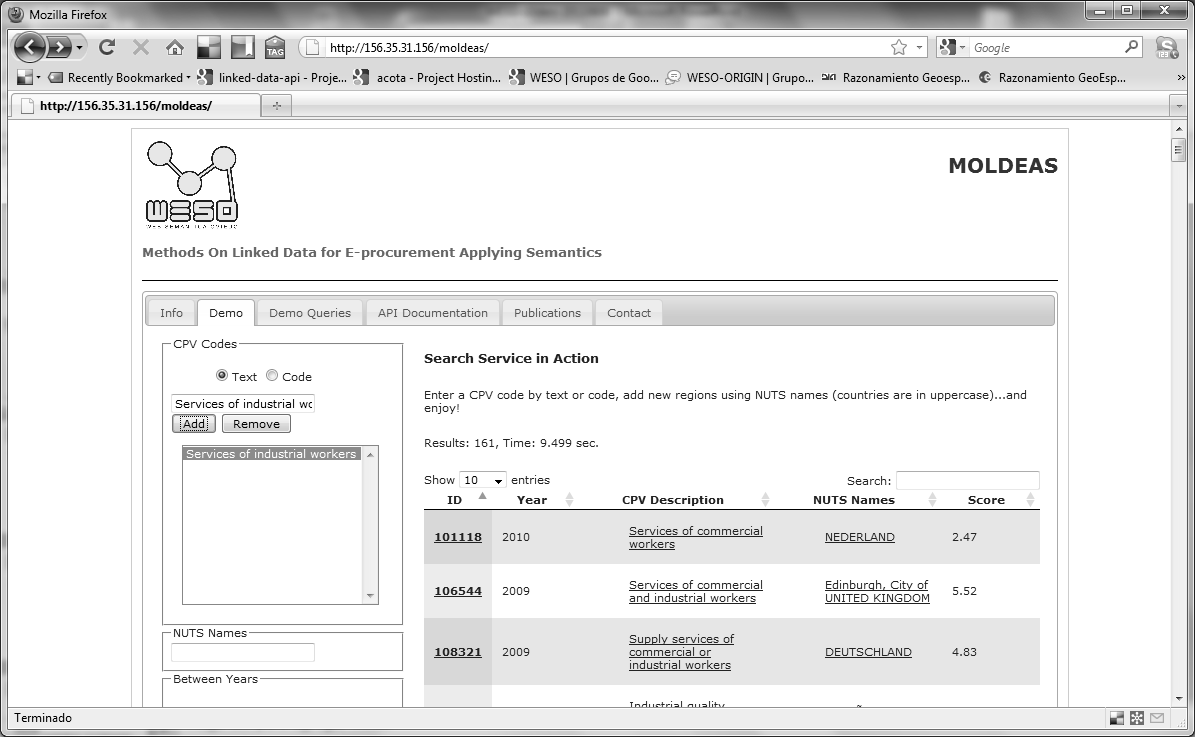
\includegraphics[width=14cm]{images/phd/moldeas/moldeas-web}
\caption{Ejemplo de pantalla inicial en \texttt{moldeas-web}.}
\label{fig:moldeas-web-screen}
\end{figure}


\item Una vez que el usuario ha seleccionado su perfil de búsqueda se ejecuta 
el proceso de recuperación de información presentando los resultados en forma 
tabular y mediante el uso de Exhibit, ver Figura~\ref{fig:moldeas-results-screen}. El usuario 
puede modificar su perfil de búsqueda y las consultas se lanzarán automáticamente una 
vez se detecten cambios. De la misma forma, el usuario puede filtrar los resultados, 
ordenarlos por relevancia, por sector, etc. e incluso visualizar la región en la 
que se han publicado los anuncios de licitación. La idea subyacente a esta 
interacción reside en que el usuario disponga del completo control de la presentación 
de los resultados obtenidos.


\begin{figure}[!htb]
\centering
	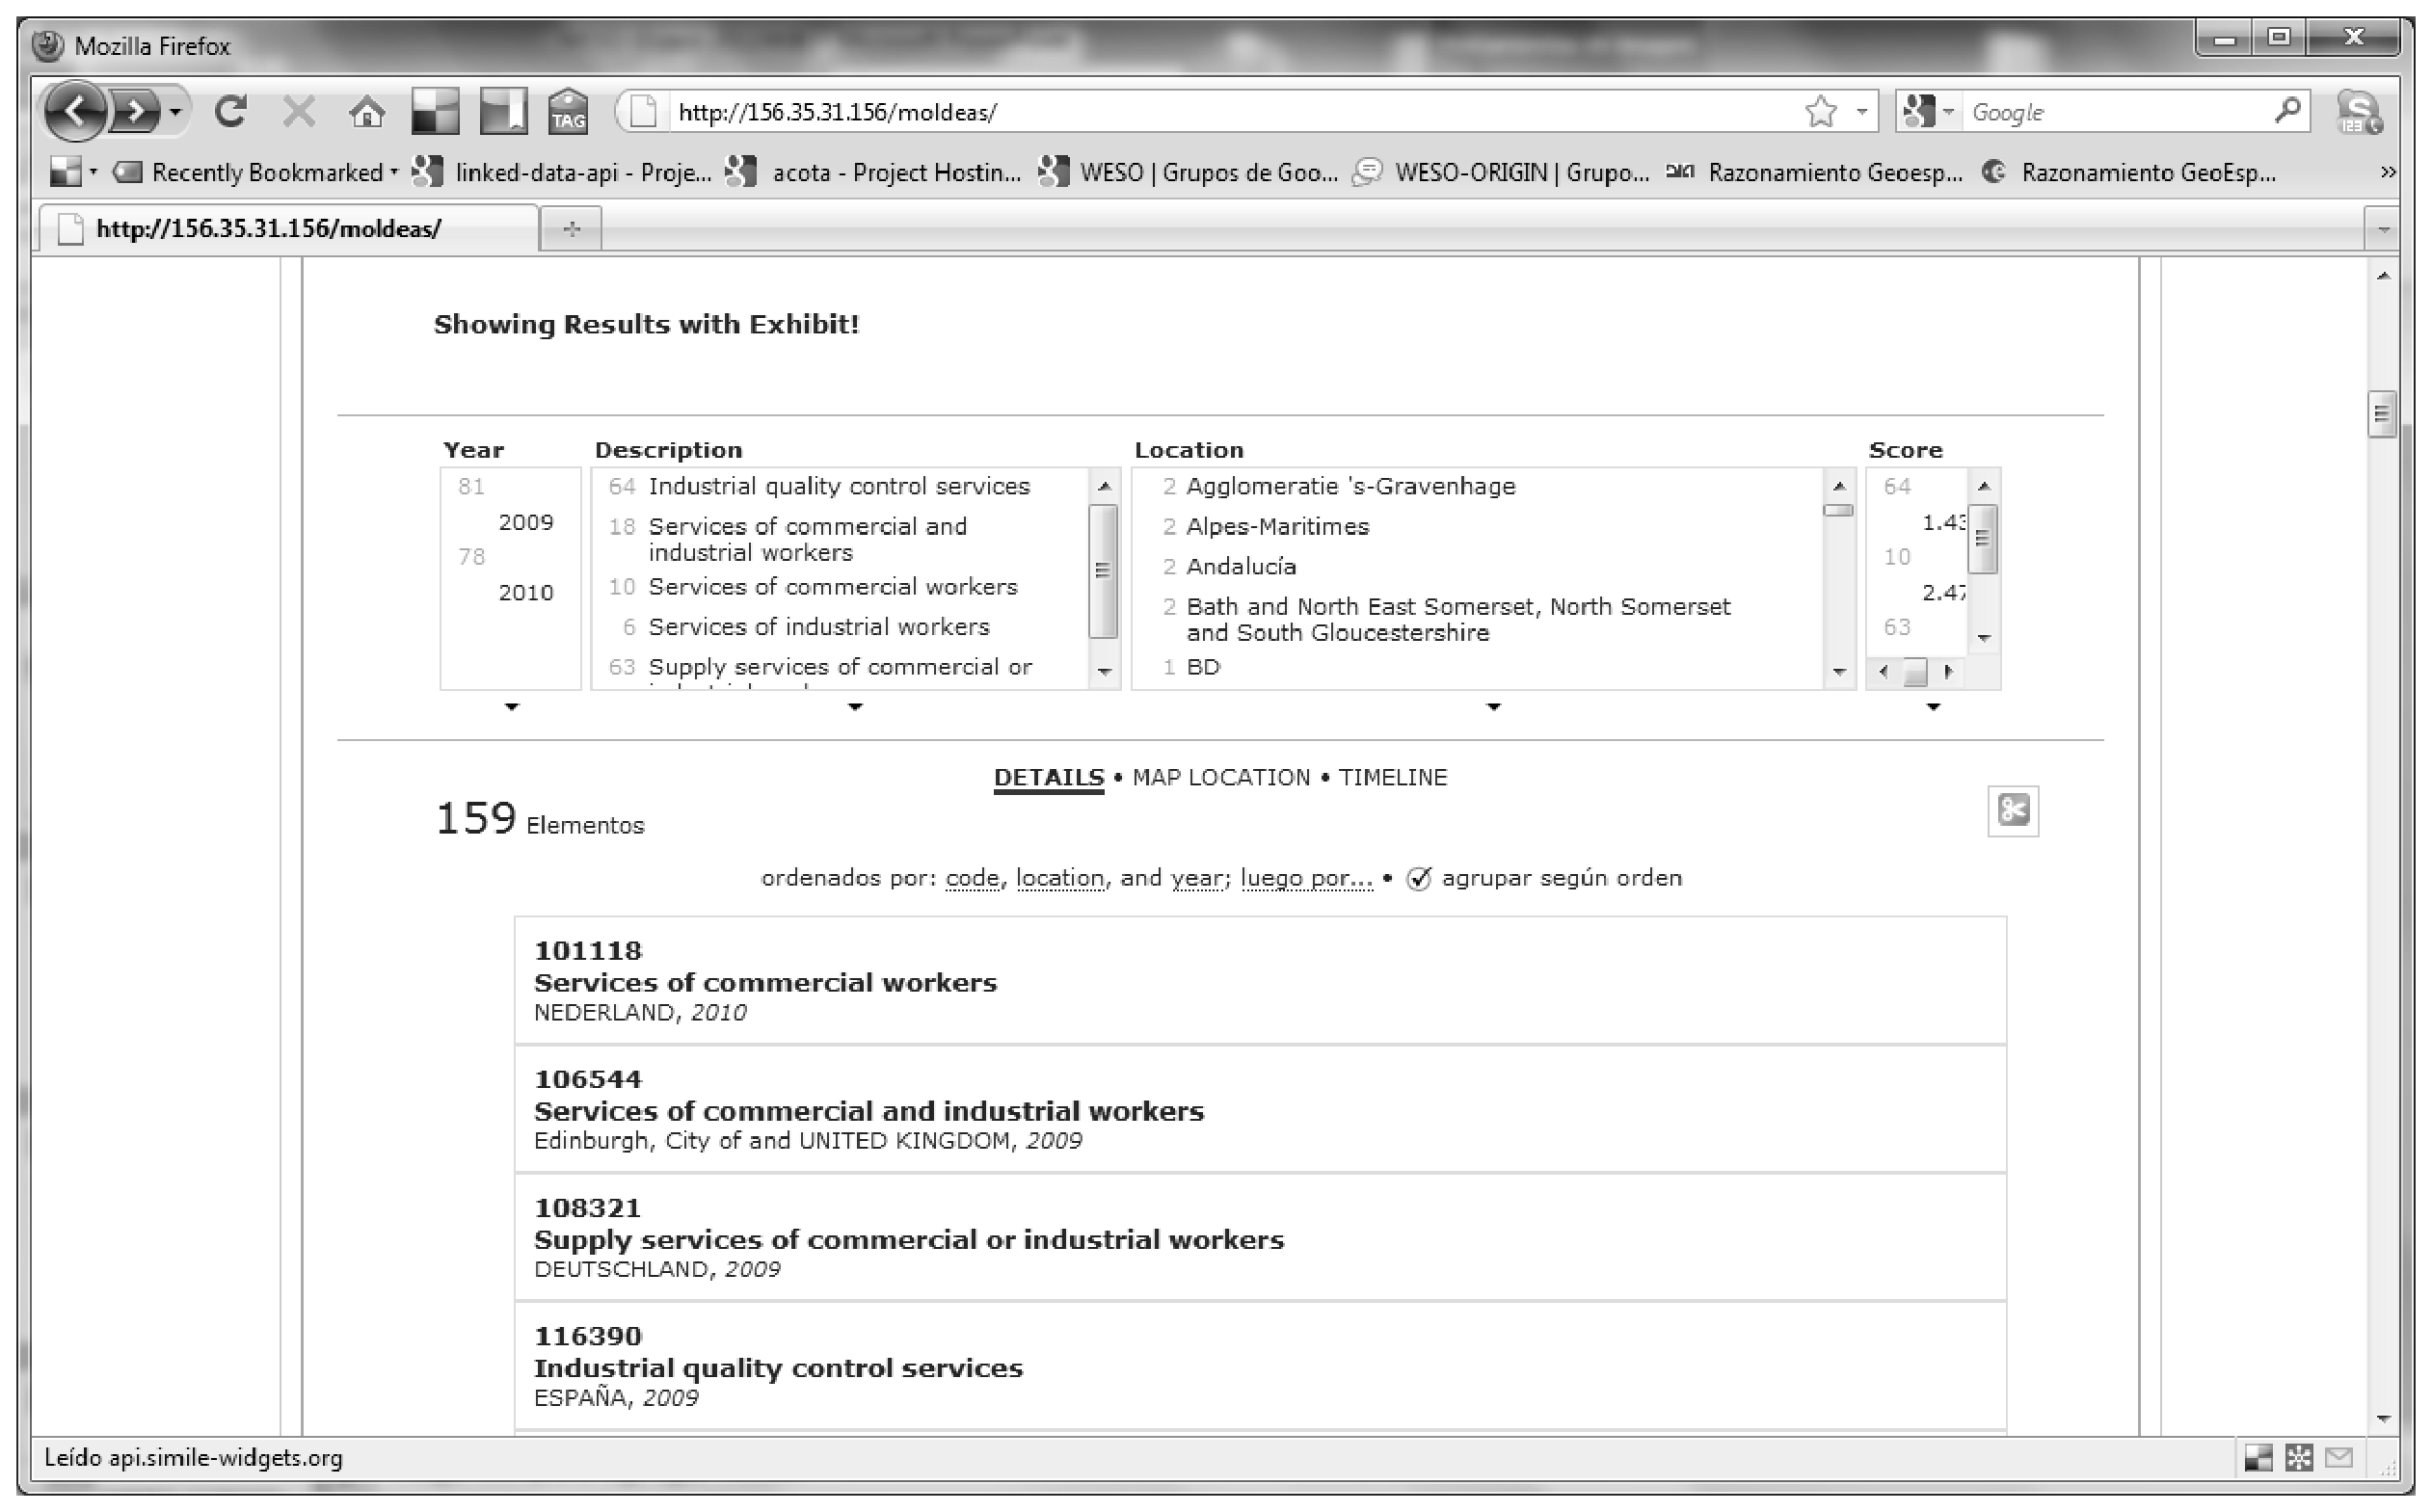
\includegraphics[width=14cm]{images/phd/moldeas/moldeas-results}
\caption{Ejemplo de pantalla de resultados en \texttt{moldeas-web}.}
\label{fig:moldeas-results-screen}
\end{figure}


\item En los resultados de búsqueda todas las \gls{URI}s presentadas son referenciables siguiendo 
las buenas prácticas de \linkeddata que han guiado la promoción de los datos a esta iniciativa. 
Es por ello que los datos propios del \dataset \gls{RDF} se pueden consultar y navegar a través de sus 
relaciones mediante el uso de un \linkeddata \textit{front-end}, en este caso Pubby, ver Figura~\ref{fig:moldeas-pubby-screen}. 


\begin{figure}[!htb]
\centering
	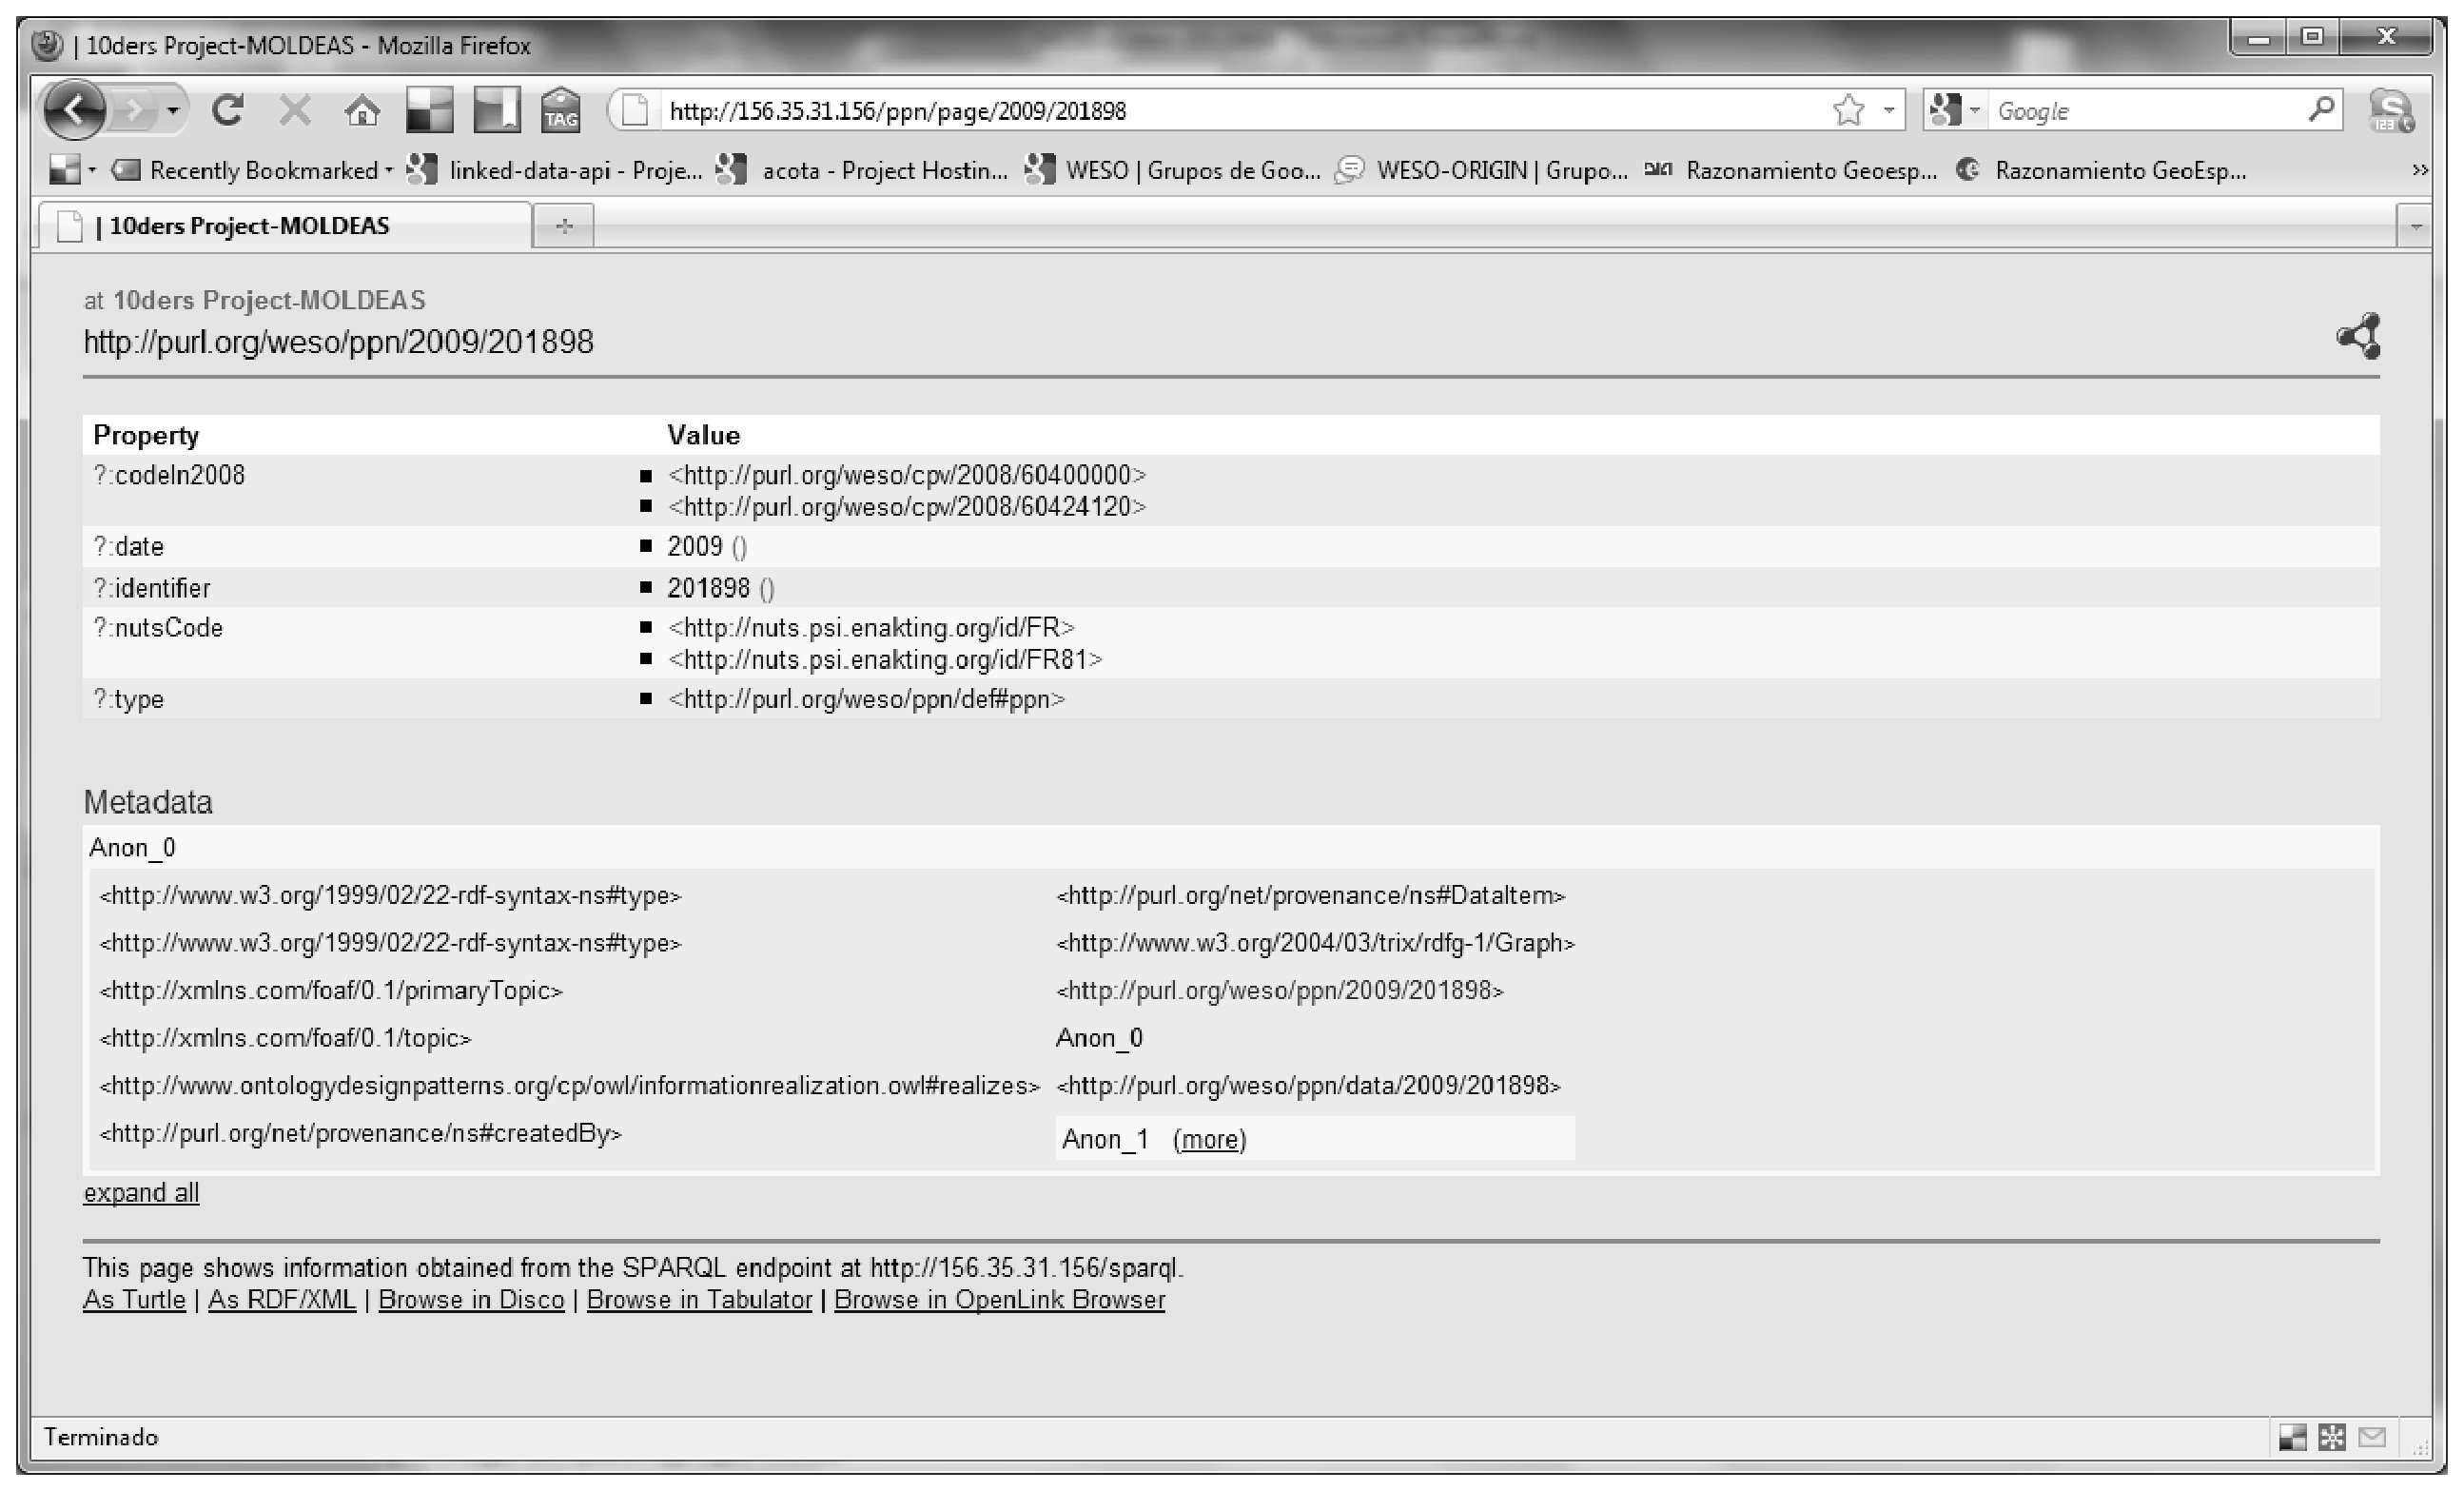
\includegraphics[width=14cm]{images/phd/moldeas/moldeas-pubby}
\caption{Acceso a los datos enlazados mediante Pubby.}
\label{fig:moldeas-pubby-screen}
\end{figure}


\item Finalmente y con el objetivo de ejemplificar el uso de \gls{SPARQL} y las posibilidades 
de consultas al \texttt{endpoint} se han creado una serie de consultas representativas 
para que los usuarios más técnicos tengan la posibilidad de configurar y crear sus propias 
consultas, ejecutándolas y obteniendo los resultados directamente. Para suministrar esta funcionalidad 
se ha utilizado la herramienta \gls{SNORQL}, ver Figura~\ref{fig:moldeas-snorql-screen}.

\begin{figure}[!htb]
\centering
	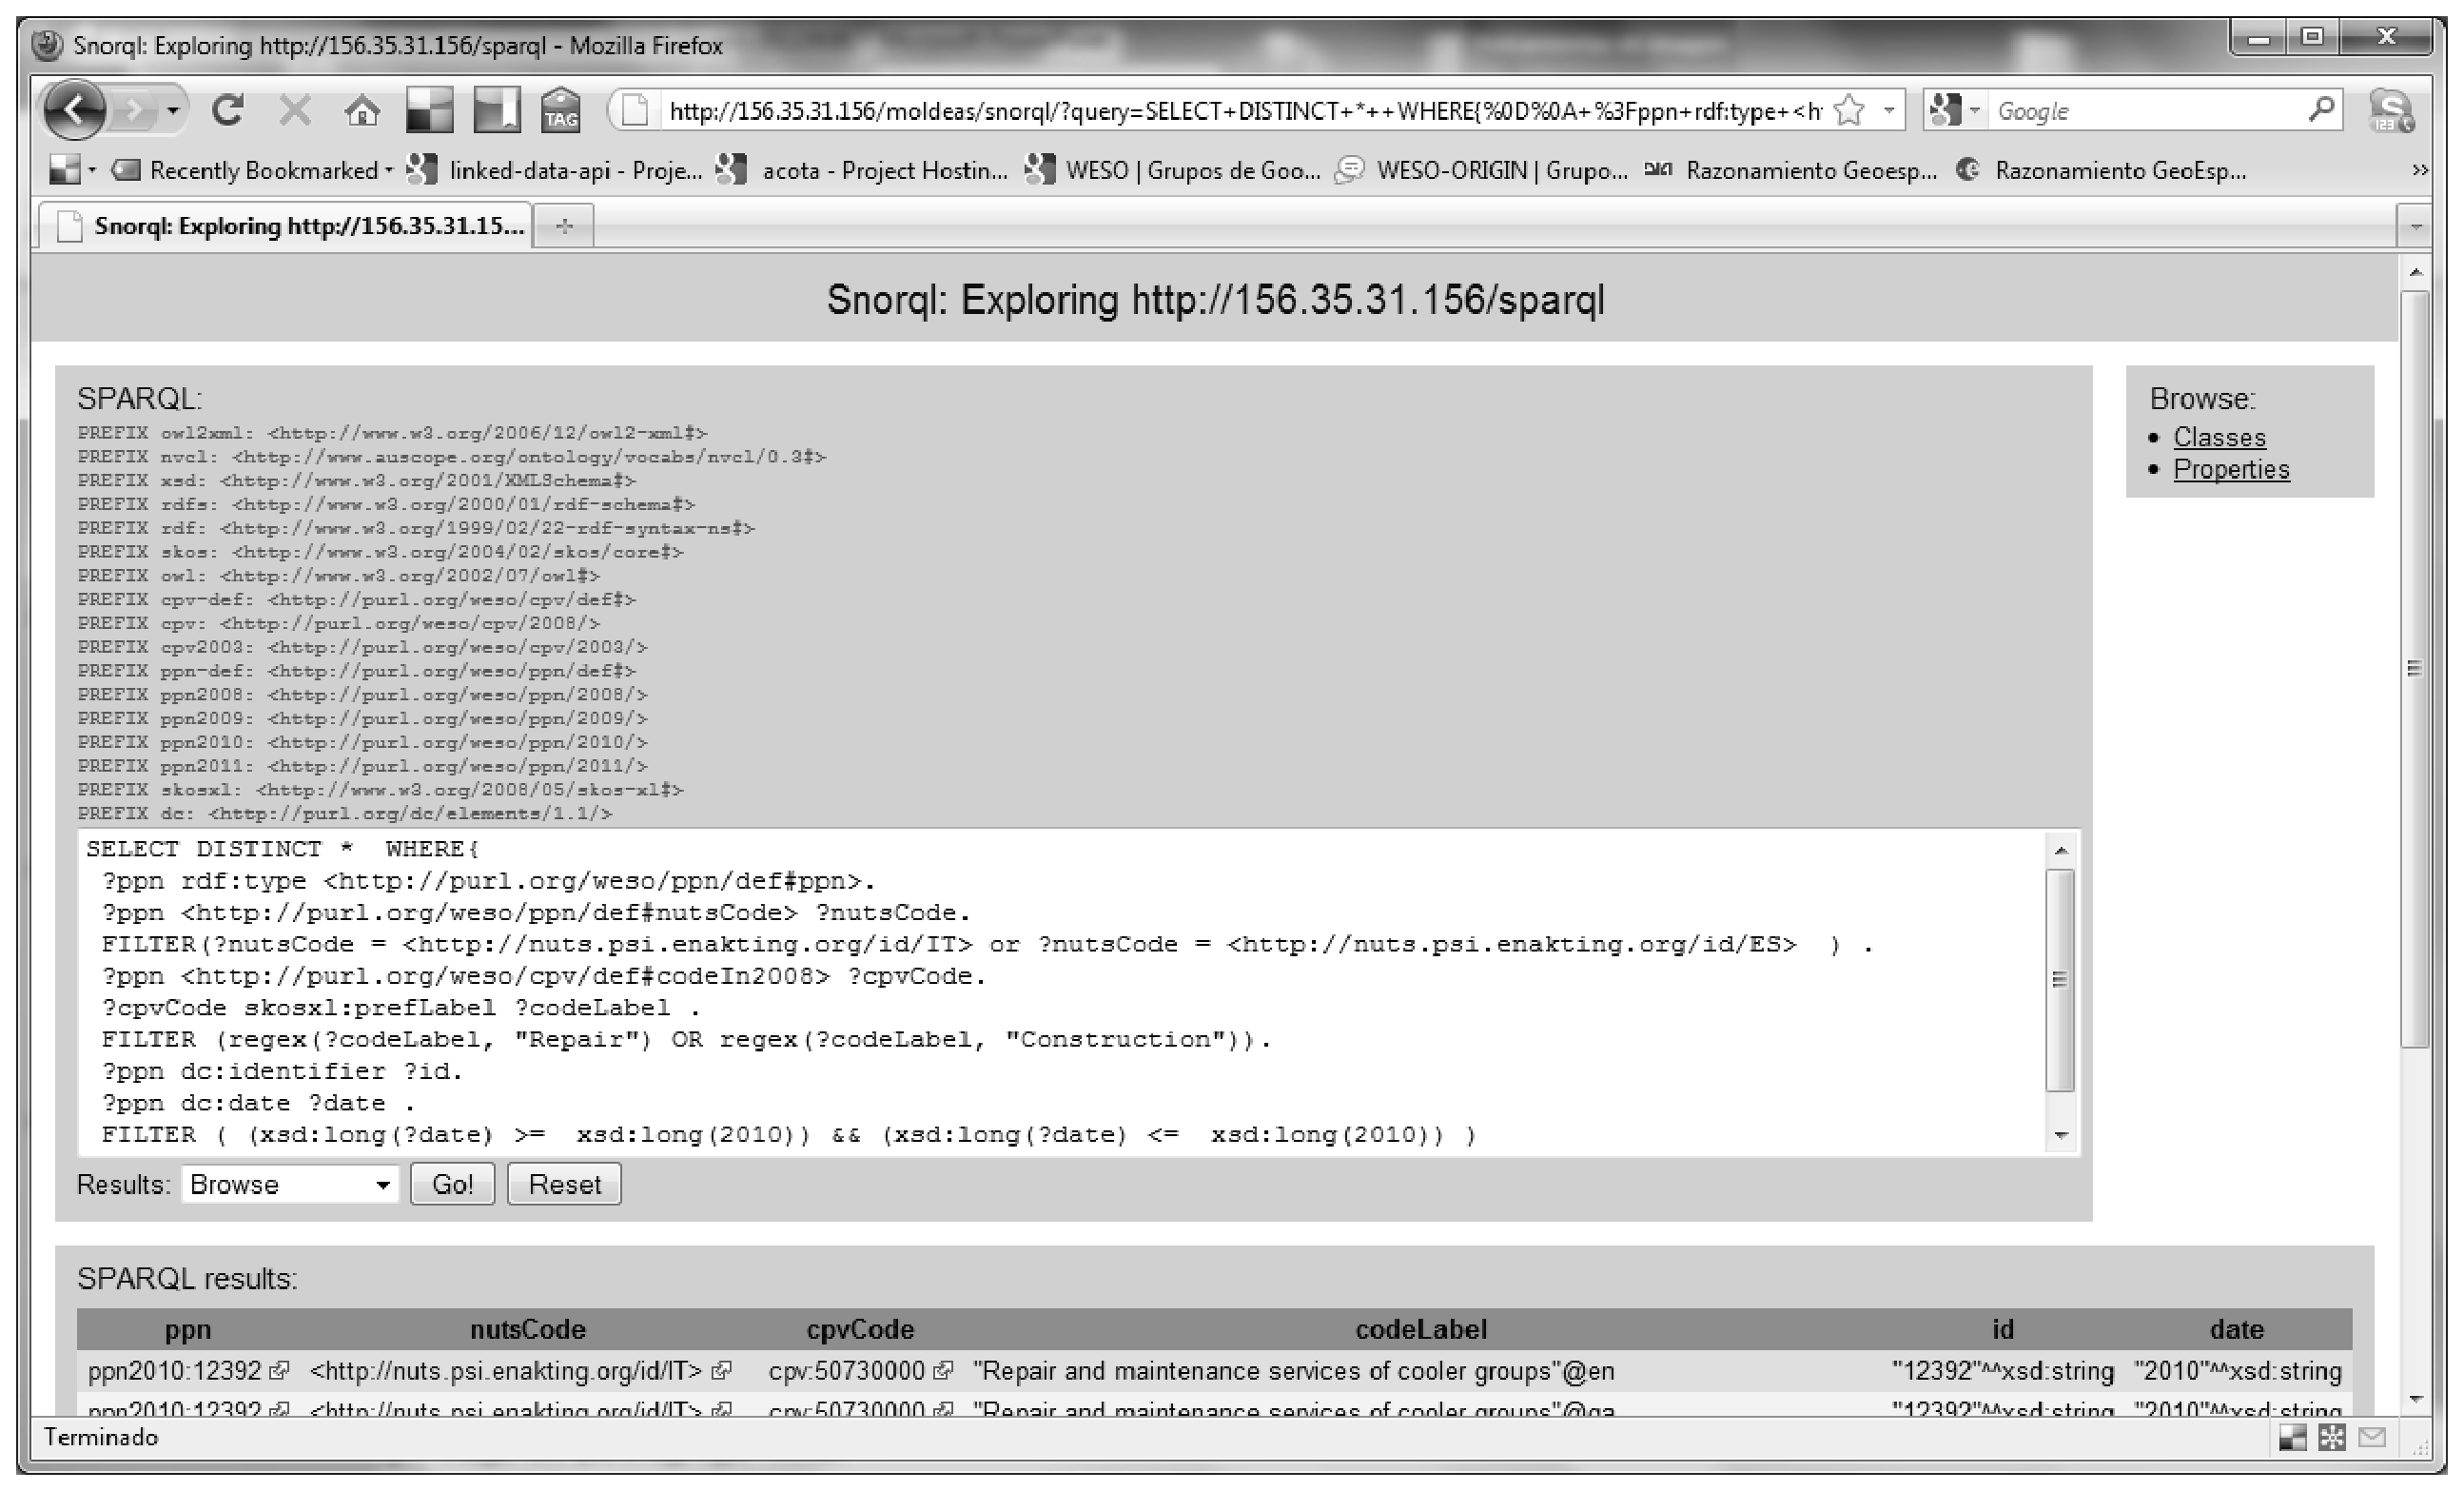
\includegraphics[width=14cm]{images/phd/moldeas/moldeas-snorql}
\caption{Consulta a los datos enlazados mediante SNORQL.}
\label{fig:moldeas-snorql-screen}
\end{figure}



\end{enumerate}









\section{Experimento sobre el Rendimiento del\\ Sistema MOLDEAS}
\subsection{Diseño del experimento sobre el Rendimiento del Sistema MOLDEAS}
El objetivo de un experimento, especialmente los estadísticos, es averiguar si unos determinados 
factores influyen en una determinada variable de interés para así poder cuantificar dicha influencia. En el caso 
de esta sección la variable a estudiar es el rendimiento de las consultas \gls{SPARQL} contra el \textit{endpoint} utilizado, si bien 
no es el experimento principal de este documento ya que conllevaría la comparación con distintos proveedores de 
repositorios \gls{RDF}, si que ha surgido la necesidad de abordar esta cuestión por la latencia en las consultas. La metodología utilizada 
para el diseño del experimento es la repetición, en condiciones indistinguibles, con el objetivo de minimizar la variabilidad 
del mismo y que el error experimental sea lo más pequeño posible.

El tratamiento del rendimiento de las consultas permite estudiar si las mejoras introducidas mejoran 
el tiempo de ejecución de las mismas partiendo de un caso básico sin ninguna optimización y a continuación, a 
través de distintas repeticiones y la introducción de optimizaciones extraer aquel conjunto de mejoras que 
permiten extraer la influencia de las características incorporadas, seleccionando así la combinación con mejores resultados. Con este objetivo, 
se ejecutan las distintas iteraciones del experimento para a través de este proceso empírico detectar 
cambios significativos en la respuesta y comprender el comportamiento del rendimiento en las consultas. Por lo tanto, 
en este caso el experimento se realiza para encontrar las condiciones con las que se consigue la optimización 
más crítica y comparar las respuestas en tiempo de ejecución con la variación de las variables, en contraposición, 
no es objetivo del experimento obtener un modelo matemático que permita realizar predicciones futuras. 

Un aspecto importante de este experimento es que la evaluación del mismo se realiza mediante los resultados obtenidos mediante 
una correcta planificación, esquivando el uso de datos históricos para no incurrir en errores debidos a la aleatoriedad. Por otra parte, 
durante la ejecución de un experimento suelen surgir distintos de variabilidades que deben ser tomadas en cuenta:
\begin{itemize}
 \item Sistemática y planificada, cuyo origen viene determinada por las diferencias sistemáticas al variar las condiciones, 
variables del experimento. Este tipo de variabilidad es conveniente y debe ocurrir para poder evaluar el experimento.
\item Debida a la naturaleza del problema y del experimento, se trata de variaciones debidas al ruido, error de medida, etc., siendo 
 impredecibles e inevitables. En el caso del experimento objeto de estudio se origina por cuestiones relacionadas con 
el tiempo de latencia en la red, etc. No obstante, esta variabilidad es medible y se puede extrapolar para la toma 
de decisiones.
\item Sistemática y no planificada, cuyo origen se debe a causas desconocidas, generando resultados sesgados. En el caso 
de estudio este tipo de variabilidad ha sido resuelta realizando las distintas réplicas en bloques de ejecución.
\end{itemize}

Una vez determinadas los puntos clave a tener en cuenta para la evaluación de los resultados es conveniente la caracterización 
propia del experimento que consta de las siguientes etapas:
\begin{enumerate}
 \item Definición de los objetivos del experimento. Las preguntas a responder por el experimento serán:
\begin{itemize}
 \item ¿Cuáles son las mejoras que se pueden aplicar sobre una consulta en SPARQL para mejorar el tiempo de ejecución?
 \item ¿Cuál es la combinación de mejoras que obtiene un mejor tiempo de respuesta?
 \item ¿Cuál es el coste de la combinación de estas mejoras? 
 \item ¿Existe algún elemento externo de configuración que implique un incremento en el tiempo de ejecución de las consultas? 
 \item ¿Cómo afectan los resultados en la implementación actual del sistema \gls{MOLDEAS}?
\end{itemize}
 \item Selección de una regla de asignación de las unidades experimentales a las condiciones de estudio. En este caso, 
la unidad experimental de este estudio será un repositorio RDF con un determinado orden de ejecución de cada uno 
de los tratamientos (variedad de consultas, casos de test $T_k$) para obtener las medidas de las observaciones, de esta forma se deben atender a los siguientes factores:
\begin{itemize}
 \item Cualitativos: tipo de entorno hardware y software, tipo de consulta en SPARQL con variaciones.
 \item Cuantitativos: tamaño de la muestra, de la memoria y número de réplicas.
\end{itemize}

En cuanto a la caracterización de los factores cualitativos, respecto al entorno hardware y software se utiliza el definido en la Sección~\ref{exp-general}. Sobre las consultas en SPARQL, existen trabajos sobre la optimización de las mismas~\cite{Schmidt2010,Bernstein07optarq:a,sparqlOpt} para la 
consulta eficiente de diferentes repositorios RDF~\cite{Yan:2008:EQR:1367497.1367652}, en este caso el tipo de consulta se centra en dos principales 
variables de información de los anuncios de licitación como son los códigos CPV (tipo) y NUTS (localización), para ello tras la ejecución de método 
de expansión de conceptos a partir de un código inicial se obtienen una serie de códigos recomendados para su posterior transformación en una 
consulta en SPARQL, la lista completa de los códigos se presenta en la Tabla~\ref{tabla:queries}. Es conveniente destacar que el método de expansión 
es independiente de esta prueba ya que simplemente se necesitan códigos independientemente de su calidad y su descripción. La selección de códigos se ha llevado a 
cabo contemplando los tipos presentes en el \gls{CPV} (División, Grupo, Clase y Categoría) estén representados ($Q_{1..8}$) además de proveer una consulta 
aleatoria $Q_9$, sobre los códigos \gls{NUTS} se han escogido aquellos representativos de países con el objetivo de generalizar y obtener un mayor nuevo 
de resultados.

\begin{table}[!ht]
\renewcommand{\arraystretch}{1.3}
\begin{center}
\begin{tabular}{|p{3cm}|p{2.5cm}|p{3.5cm}|p{3.5cm}|}
\hline
  \textbf{ID Consulta} & \textbf{Código CPV inicial} & \textbf{Códigos CPV expandidos} & \textbf{Códigos NUTS}  \\ \hline
  $Q_1$ & 15331137 & 48611000, 48611000, 50531510, 15871210 & UK, PL, RO \\ \hline
  $Q_2$ & 50531510 & 34144100, 44212211, 44212212, 50531500 & ES, FR, DE \\ \hline
  $Q_3$ & 34144100 & 44212211, 31140000, 31140000, 34144100 & PL, CZ, RO \\ \hline
  $Q_4$ & 64122000 & 64216120, 79571000, 15871210, 64121000 & BE, SE, DE \\ \hline
  $Q_5$ & 79320000 & 75241000, 75100000, 75000000, 60112000 & UK, FR, AT \\ \hline
  $Q_6$ & 44100000 & 44110000, 44170000, 44190000, UB03 & NL, SE, DE \\ \hline
  $Q_7$ & 31000000 & 33141000, 39000000, 44000000, 31600000 & DE, IT, HU \\ \hline
  $Q_8$ & 50000000 & 50512000, 50333100, 50530000, 50532300 & UK, IR, FR \\ \hline
  $Q_9$ (random)   & 15841400 & 15841300, 15511700, 44921210, 03131400 & ES, FR, DK \\ \hline
  \hline
  \end{tabular}
  \caption{Descripción de los códigos en las consultas en SPARQL del experimento.}
  \label{tabla:queries}
  \end{center}
\end{table} 

En referencia a los aspectos cuantitativos del experimento, el tamaño de la muestra consta de nueve consultas ($Q_{1..9}$), el número de réplicas 
para evitar el ruido y la aleatoriedad previamente comentada es de $3$ y la situación de partida para cada una de ellas se produce 
bajo las mismas condiciones: reinicio de la máquina y $18$ consultas de entrenamiento (1 simple y 1 expandida) antes de la ejecución de una réplica para la obtención 
de las observaciones de tiempo de ejecución. Referente al tamaño de la muestra, se utilizará el \textit{endpoint} descrito anteriormente y con la carga 
de tripletas generada a partir de la aplicación de los métodos semánticos a los anuncios de licitación y siguiendo la distribución por 
grafos nombrados especificada en el Sección FIXME.

Por otra parte, las características, $F_i$, a evaluar en combinación se presentan en la siguiente Tabla~\ref{table:sparql-features}, en resumen se parte de una 
consulta simple (1 código CPV y 1 código NUTS) para obtener un tiempo de referencia, a partir de esta primera referencia se aplican 
las distintas optimizaciones, generando los distintos tratamientos ($T_i$), ver Tabla~\ref{tabla:tests}, para el establecimiento de la mejor combinación posible.

\begin{longtable}[c]{|l|p{10cm}|} 
\hline
\textbf{ID} &  \textbf{Descripción}  \\\hline
\endhead
$F_1$ & Consulta simple: $1$ código CPV y $1$ código NUTS \\ \hline
$F_2$ & $F_1$ con uso de la clausula \texttt{LIMIT} de SPARQL \\ \hline
$F_3$ & Consulta expandida: $n$ códigos CPV y $n$ código NUTS  \\ \hline
$F_4$ & Rescritura de las consultas SPARQL: \texttt{FILTER}, etc.  \\ \hline
$F_5$ & Uso de grafos nombrados en la consulta SPARQL: claúsula \texttt{FROM} \\ \hline
$F_6$ & Separación de las consultas en SPARQL en simples ($F_1$) \\ \hline
$F_7$ & Consultas simples distribuidas con $5$ hilos (1 por código CPV) \\ \hline
\hline
\caption{Características de las consultas en SPARQL.}\label{table:sparql-features}\\    
\end{longtable}

\newpage 

\begin{table}[!htb]
\renewcommand{\arraystretch}{1.3}
\begin{center}
\begin{tabular}{|p{3.5cm}|p{0.8cm}|p{0.8cm}|p{0.8cm}|p{0.8cm}|p{0.8cm}|p{0.8cm}|p{0.8cm}|p{2cm}|}
\hline
  \textbf{Test}/ \textbf{Característica}& \textbf{$F_1$} & \textbf{$F_2$} & \textbf{$F_3$} & \textbf{$F_4$} & \textbf{$F_5$} & \textbf{$F_6$} &  \textbf{$F_7$} & \textbf{Nº consultas SPARQL} \\ \hline
   $T_1$ & $\star$ & & & & & & &$1$\\ \hline 
   $T_2$ & $\star$ & & $\star$ & & & & &$1$\\ \hline 
   $T_3$ &  & $\star$ &  & & & & &$1$\\ \hline 
   $T_4$ &  & $\star$ & $\star$ & & & & &$1$\\ \hline 
   $T_5$ &  & $\star$ & $\star$ & $\star$ & & & &$1$\\ \hline 
   $T^{1}_6$ ($n$ códigos CPV y $m$ códigos NUTS)&  & $\star$ & $\star$ & $\star$ & $\star$ & $\star$ & &$4$\\ \hline 
   $T^{2}_6$ ($\equiv$)&  & $\star$ & $\star$ & $\star$ & $\star$ & $\star$ & $\star$ &$4$\\ \hline 
   $T^{1}_7$ ($1$ código CPV y $m$ códigos NUTS) &  & $\star$ & $\star$ & $\star$ &  & $\star$ &  &$5$ \\ \hline 
   $T^{2}_7$ ($\equiv$) & & $\star$ & $\star$ & $\star$ &  & $\star$ & $\star$ &$5$\\ \hline 
   $T^{1}_8$ ($\equiv$)& & $\star$ & $\star$ & $\star$ & $\star$ & $\star$ &  &$20$\\ \hline 
   $T^{2}_8$ ($\equiv$) & & $\star$ & $\star$ & $\star$ & $\star$ & $\star$ &  $\star$ &$20$\\ \hline 
   $T^{1}_9$ ($1$ código CPV y $1$ código NUTS ) & & $\star$ & $\star$ & $\star$ &  & $\star$ & &$15$  \\ \hline 
   $T^{2}_9$ ($\equiv$)& & $\star$ & $\star$ & $\star$ & & $\star$ &  $\star$ &$15$\\ \hline 
   $T^{1}_{10}$ ($\equiv$) & & $\star$ & $\star$ & $\star$ & $\star$ & $\star$ & &$60$  \\ \hline 
   $T^{2}_{10}$ ($\equiv$) & & $\star$ & $\star$ & $\star$ & $\star$ & $\star$ & $\star$ &$60$ \\ \hline 
  \hline
  \end{tabular}
  \caption{Descripción de cada uno de los tratamientos, características de optimización.}
  \label{tabla:tests}
  \end{center}
\end{table} 

 \item Especificación de las medidas de trabajo en cuanto a la respuesta. El valor que se toma es el tiempo de ejecución 
en segundos de la consulta en SPARQL. 
 \item Ejecución de un experimento piloto. Evidentemente esta tarea se ha realizado con una pequeña muestra de consultas, sólo un año de anuncios 
de licitación pero ejecutando todos los tratamientos con el fin de validar el enfoque propuesto, obtener los resultados de toma de tiempos y preparar 
el procesamiento del registro de tiempos para obtener las medidas finales.
 \item Especificación de un modelo. En este caso, no se utilizará un modelo matemático para aproximar los valores 
como ya se ha explicado anteriormente debido a que el objetivo es optimizar la realización de consultas, en cuanto a 
tiempo de ejecución, no la predicción futura.
 \item Esquematización de los pasos a seguir.
 \item Determinación del tamaño muestral. Como ya se ha comentado anteriormente, en el apartado de factores cuantitativos, se utilizarán los datos generados durante el proceso de promoción 
de datos a \linkeddata de los anuncios de licitación y de las clasificaciones de productos.
 \item Revisión de las decisiones anteriores.
\end{enumerate}

\subsection{Ejecución del experimento sobre el Rendimiento del Sistema MOLDEAS}
La aplicación del plan previsto en la anterior sección arroja un conjunto de valores para cada uno de los tratamientos ($T_k$) y réplicas de los tiempos 
de ejecución de las consultas de acuerdo a las distintas características ($F_i$). En la Tabla~\ref{tabla:tests-agregado} se reflejan 
las medias de tiempo y ganancia agregadas de cada uno de los tratamientos realizados. Por otra parte, se presentan igualmente 
las medidas pormenorizadas de las observaciones realizadas y agregadas de las 3 réplicas ejecutadas, ver Tablas~\ref{tabla:results-1} y~\ref{tabla:results-2}. 
El cálculo de la ganancia se realiza mediante la fórmula: $t_{old}/t_{new}-1*100$, tomando como referencia para $T_2$ el tiempo de $T_1$ y para 
los tratamientos $T_{4..10}$ el tiempo de $T_3$. Finalmente, la ejecución de todos los tratamientos con las distintas observaciones y 
réplicas ha implicado la realización de $5751$ consultas en SPARQL más las de entrenamiento para cada una de las réplicas. 

\begin{table}[!htb]
\renewcommand{\arraystretch}{1.3}
\begin{center}
\begin{tabular}{|l|c|c|}
\hline
  \textbf{Test}& \textbf{$\bar{X}$ Tiempo (seg.)} & \textbf{$\bar{X}$ Ganancia (\%)} \\ \hline
   $T_1$ & $3.21$  & N/A\\ \hline 
   $T_2$ & $3.25$  & $1.21$   \\ \hline 
   $T_3$ & $20.548$ & N/A   \\ \hline 
   $T_4$ & $20.552$ & $-0.02$ \\ \hline 
   $T_5$ & $20.545$ & $-0.01$ \\ \hline 
   $T^{1}_6$ & $20.52$  & $0.14$\\ \hline 
   $T^{2}_6$ & $11.80$ & $74.37$\\ \hline 
   $T^{1}_7$ & $15.81$ & $30.58$ \\ \hline 
   \textbf{$T^{2}_7$} & \textbf{$10.51$} & \textbf{$96.54$} \\ \hline
   $T^{1}_8$ & $32.33$ & $-36.11$ \\ \hline 
   $T^{2}_8$ & $18.45$ & $11.21$ \\ \hline 
   $T^{1}_9$ & $22.53$ & $-8.77$ \\ \hline 
   $T^{2}_9$ & $12.61$ & $63.36$ \\ \hline 
   \textbf{$T^{1}_{10}$} & \textbf{$71.01$} & $-70.97$ \\ \hline 
   $T^{2}_{10}$ & $35.08$ & $-40.42$ \\ \hline 
  \hline
  \end{tabular}
  \caption{Tiempo de ejecución (seg.) y ganancia (\%).}
  \label{tabla:tests-agregado}
  \end{center}
\end{table} 



\begin{table}[!h]
\renewcommand{\arraystretch}{1.3}
\begin{center}
\begin{tabular}{|p{1.5cm}|p{1.5cm}|p{1.5cm}|p{1.5cm}|p{1.5cm}|p{1.5cm}|p{1.5cm}|p{1.5cm}|}
\hline
\textbf{ID Consulta/ Test} & $T_1$ & $T_2$ & $T_3$ & $T_4$ & $T_5$ & $T^{1}_{6}$ & $T^{2}_{6}$ \\ \hline
  $Q_1$ & $3.21$ (NA) & $3.13$ ($2.46$) & $19.35$ (NA) & $19.53$ ($-0.91$) & $19.45$ ($0.49$)  & $19.24$ ($0.58$) & $11.16$ ($73.49$)\\ \hline
  $Q_2$ & $3.15$ (NA) & $3.14$ ($0.52$) & $23.56$ (NA)   & $23.68$ ($-0.52$)  & $23.68$ ($0.52$) & $24.06$ ($-2.10$) & $13.24$ ($77.95$) \\ \hline
  $Q_3$ & $3.14$ (NA)  & $3.14$ ($0.11$) & $18.56$ (NA)  & $18.47$ ($0.46$)  & $18.44$ ($-0.60$)  & $18.69$ ($-0.71$)  & $10.08$ ($84.14$) \\ \hline
  $Q_4$ & $3.16$ (NA)  & $3.13$ ($0.79$) & $18.52$ (NA)  & $18.32$ ($1.08$)  & $18.50$ ($-0.10$)  & $18.20$ ($1.77$)  & $10.19$ ($81.73$) \\ \hline
  $Q_5$ & $3.29$ (NA)  & $3.17$ ($3.82$) & $22.69$ (NA)  & $22.85$ ($-0.72$)  & $22.69$ ($0.01$)  & $22.62$ ($0.31$)  & $14.61$ ($55.31$) \\ \hline
  $Q_6$ & $3.21$ (NA)  & $3.17$ ($1.35$) & $18.55$ (NA)  & $18.45$ ($0.51$)  & $18.48$ ($-0.35$)  & $18.22$ ($1.78$)  & $10.00$ ($85.46$) \\ \hline
  $Q_7$ & $3.39$ (NA)  & $3.39$ ($0.25$) & $19.01$ (NA)  & $19.19$ ($-0.93$)  & $19.12$ ($0.55$)  & $18.99$ ($0.09$)  & $11.08$ ($71.56$) \\ \hline
  $Q_8$ & $3.94$ (NA)  & $3.98$ ($-0.95$)& $23.44$ (NA)  & $23.15$ ($1.26$)  & $23.24$ ($-0.82$)  & $23.50$ ($-0.29$)  & $14.72$ ($59.24$) \\ \hline
  $Q_9$ & $3.17$ (NA)  & $3.09$ ($2.59$) & $22.23$ (NA)  & $22.32$ ($-0.40$)  & $22.27$ ($0.19$)  & $22.26$ ($-0.15$)  & $12.32$ ($80.45$) \\ \hline
  \hline
  \end{tabular}
  \caption{Tiempo de ejecución (seg.) y ganancia (\%). Parte 1.}
  \label{tabla:results-1}
  \end{center}
\end{table} 


\begin{sidewaystable}[ht!]
\renewcommand{\arraystretch}{1.3}
\begin{center}
\begin{tabular}{|p{1.5cm}|p{1.5cm}|p{1.5cm}|p{1.5cm}|p{1.5cm}|p{1.5cm}|p{1.5cm}|p{1.5cm}|p{1.5cm}|p{1.5cm}|}
\hline
\textbf{ID Consulta/ Test} & $T^{1}_{7}$ & $T^{2}_{7}$ & $T^{1}_{8}$ & $T^{2}_{8}$ & $T^{1}_{9}$ & $T^{2}_{9}$ & $T^{1}_{10}$ & $T^{2}_{10}$\\ \hline
  $Q_1$ & $15.71$ ($23.18$)  & $10.62$ ($82.25$) & $33.27$ ($-41.84$) & $18.75$ ($3.24$) & $21.58$ ($-10.33$) & $12.38$ ($56.28$) & $69.13$ ($-72.00$) & $33.41$ ($-42.07$) \\ \hline
  $Q_2$ & $15.64$ ($50.57$)  & $9.90$ ($137.84$) & $32.26$ ($-26.98$) & $17.96$ ($25.66$ ) & $26.27$ ($-10.34$) & $15.50$ ($51.97$) & $73.62$ ($-68.00$) & $37.50$ ($-29.49$) \\ \hline
  $Q_3$ & $15.54$ ($19.44$)  & $9.66$ ($92.13$ ) & $32.04$ ($-42.09$) & $17.94$ ($3.29$) & $20.32$ ($-8.68$) & $10.44$ ($77.68$) & $68.95$ ($-73.09$ ) & $32.95$ ($-50.52$) \\ \hline
  $Q_4$ & $15.87$ ($16.68$)  & $9.99$ ($85.45$) & $32.07$ ($-42.24$) & $18.43$ ($3.24$) & $20.48$ ($-9.54$) & $10.33$ ($79.23$) & $68.85$ ($-73.10$) & $34.27$ ($-43.79$) \\ \hline
  $Q_5$ & $16.18$ ($40.22$)  & $11.92$ ($90.39$) & $32.46$ ($-30.10$) & $19.02$ ($23.12$) & $24.28$ ($-6.57$) & $14.40$ ($57.55$) & $74.02$ ($-69.35$ ) & $37.08$ ($-33.79$) \\ \hline
  $Q_6$ & $15.76$ ($17.73$)  & $9.60$ ($93.21$) & $32.11$ ($-42.23$) & $18.24$ ($-2.48$) & $20.51$ ($-9.55$) & $10.77$ ($72.23$) & $72.28$ ($-74.34$ ) & $32.80$ ($-49.98$) \\ \hline
  $Q_7$ & $15.93$ ($19.31$)  & $11.23$ ($69.35$ ) & $32.21$ ($-40.99$) & $18.51$ ($4.23$) & $21.12$ ($-10.01$) & $11.27$ ($68.67$) & $69.02$ ($-72.46$) & $33.55$ ($-42.04$) \\ \hline
  $Q_8$ & $16.12$ ($45.43$)  & $12.11$ ($93.54$ ) & $32.55$ ($-28.01$) & $19.50$ ($26.61$) & $25.33$ ($-7.48$) & $16.16$ ($45.05$) & $72.72$ ($-67.77$) & $38.27$ ($-30.16$) \\ \hline
  $Q_9$ & $15.58$ ($42.66$)  & $9.89$ ($124.71$) & $31.99$ ($-30.51$) & $17.74$ ($14.01$) & $23.76$ ($-6.46$) & $13.76$ ($61.57$) & $70.76$ ($-68.59$) & $36.40$ ($-41.92$) \\ \hline
  \hline
  \end{tabular}
  \caption{Tiempo de ejecución (seg.) y ganancia (\%). Parte 2.}
  \label{tabla:results-2}
  \end{center}
\end{sidewaystable} 


Adicionalmente, los resultados agregados de este experimento, respecto a los tratamientos de referencia $T_1$ y $T_3$, 
se visualizan gráficamente en las siguientes gráficas, ver Figuras~\ref{fig:results-graph-1} y~\ref{fig:results-graph-2} 
tomando como referencia el tiempo de ejecución y Figura~\ref{fig:results-graph-3} presentando la ganancia en porcentaje respecto a $T_3$.

\begin{figure}[!htb]
\centering
	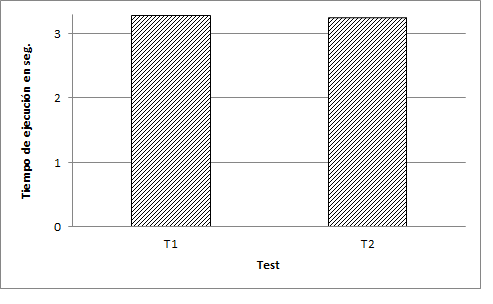
\includegraphics[width=12cm]{./images/phd/experimentation/t1-t2-tiempo}
\caption{Gráfica de Tiempo de ejecución medio con referencia $T_1$.}
\label{fig:results-graph-1}
\end{figure}

\begin{figure}[!htb]
\centering
	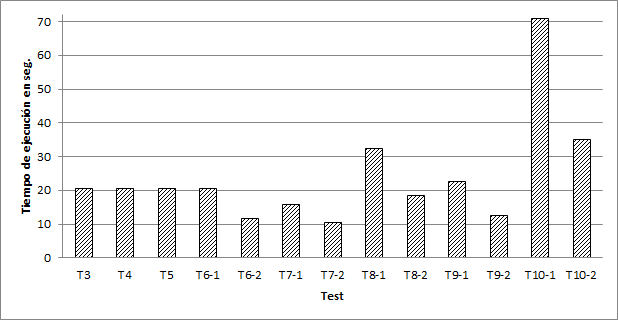
\includegraphics[width=14cm]{./images/phd/experimentation/t3-t10-tiempo}
\caption{Gráfica de Tiempo de ejecución medio con referencia $T_3$.}
\label{fig:results-graph-1}
\end{figure}

\begin{figure}[!htb]
\centering
	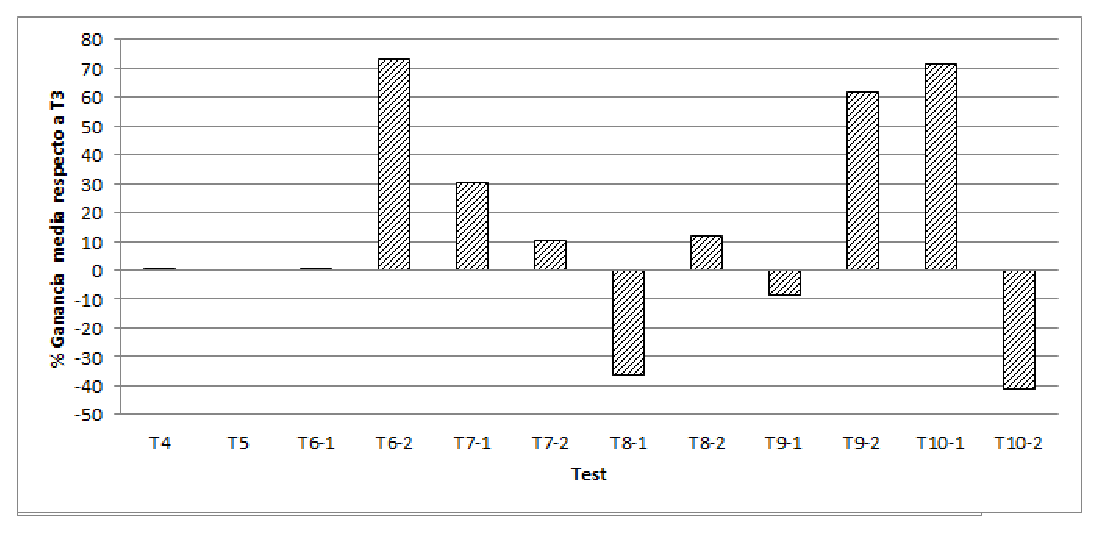
\includegraphics[width=14cm]{./images/phd/experimentation/t3-t10-ganancia}
\caption{Gráfica de Ganancia media con referencia $T_3$ en (\%).}
\label{fig:results-graph-2}
\end{figure}

\subsection{Validación del experimento sobre el Rendimiento del Sistema MOLDEAS}
La realización del experimento de rendimiento de las consultas en \gls{SPARQL} es motivado por el exceso 
de latencia en las consultas al repositorio \gls{RDF}. Como ya se ha mencionado no es objetivo la comparación 
de distintos repositorios RDF para comprobar cuál obtiene un mejor rendimiento para las consultas realizadas 
sino probar cuáles son las optimizaciones en las consultas en SPARQL y en el código fuente del demostrador que 
permiten acelerar el tiempo de la consulta independientemente del proveedor del servicio. Por ello, las características 
a combinar $F_i$ para obtener un mejor tiempo de respuesta permiten establecer la mejor conjunción de las mismas de acuerdo 
al estudio de los tiempos de ejecución obtenidos. 

De acuerdo a los resultados obtenidos se establecen los siguientes puntos clave y conclusiones:
\begin{itemize}
\item Los tipos de consulta generados a partir de $F_1$ y $F_3$ permiten establecer un valor de referencia 
en tiempo de ejecución para su posterior comparación con las mejoras introducidas. De esta manera se establece 
un primer valor de referencia para la comparación de consultas simples ($1$ código CPV y $1$ código NUTS) entorno 
a los $3$ segundos y otro para consultas expandidas, $n$ códigos CPV y $n$ código NUTS, en torno a los $20$ segundos. Estos 
valores son un por una parte motivadores del experimento de mejora y por otra permiten evidenciar la ganancia con la introducción 
de nuevas características 
 \item Existen algunas de las características, $F_2$ y $F_4$, que no implican mejora en el tiempo de ejecución. 
\item En el caso particular de $F_3$, uso de la clausula LIMIT, su valor se fija en $10,000$ y carece de representatividad debido a que los resultados 
de la consulta ya son previamente filtrados y no superan esta cifra.
\item La reescritura de consultas, $F_4$, habitualmente implica mejoras en el tiempo de ejecución pero no se ha apreciado una mejora 
crítica debido a que este tipo de optimizaciones obtienen una mejora crítica cuando las consultas en SPARQL realizan operaciones 
con valores opcionales, clausula OPTIONAL, por ejemplo cuando se trasladan consultas del tipo NATURAL JOIN e INNER JOIN en SQL a SPARQL, en el 
caso de estudio estos valores no se han utilizado ya que las consultas generadas por el sistema no incluyen encaja de patrones 
mediante clausulas opcionales.
\item En cuanto a la característica $F_5$ sobre el uso de grafos nombrados se obtiene una mejora relevante ya que la selección 
de los grafos sobre los cuales se realizan las consultas permite acotar el número de tripletas, no es lo mismo realizar sobre el 
grafo RDF completo presente en el \textit{endpoint} que sobre un subconjunto del mismo. Sin embargo, hay que destacar que la 
ejecución de múltiples consultas (separando por grafo) provoca que el tiempo de ejecución sea incrementado.
\item Sin duda la mejora más intensa en cuanto a tiempo de ejecución se produce en los casos $F_6$ y $F_7$ como se puede 
ver en los tratamiento $T^{2}_6$, $T^{1}_7$, $T^{2}_7$ y $T^{2}_9$ ya que el tiempo de ejecución de consultas simples 
es relativamente bajo y, evidentemente, la distribución de consultas permite la obtención de un mejor tiempo de ejecución 
global. No obstante, en los tratamientos $T^{1}_{10}$ and $T^{2}_{10}$ esta supuesta mejora se convierte en un inconveniente 
ya que el número de consultas generadas es muy alto y la distribución mediante $5$ hilos no permite realizar una mejora.
\item Teniendo en cuenta los puntos anteriores cabe destacar que el tipo de códigos CPV no tiene ninguna implicación para 
la ejecución de la consulta. Sin embargo, el número de códigos \gls{CPV} si implica un incremento en el tiempo de ejecución, del orden 
de $3$ segundos adicionales por cada código CPV nuevo, en cambio el uso de varios códigos NUTS no supone un incremento en el tiempo 
de ejecución y en el experimento la ejecución de un código CPV con varios \gls{NUTS} es similar a la combinación $n-m$ de los mismos.
\end{itemize}

A la vista de las conclusiones extraídas y de los resultados obtenidos se comprueba que la mejora combinación de características se 
genera en el tratamiento $T^{2}_7$ con un tiempo de ejecución de $10.55$ segundos y una ganancia respecto a  $T_3$ del $95.73 \%$, la descripción 
de esta mejora implica que se trata de una consulta expandida ($F_3$) en la cual se utilizan clausulas LIMIT ($F_2$), se reescriben 
las consultas mediante FILTERs ($F_4$), generando consultas simples en SPARQL ($F_6$) de 1 código CPV y $m$ códigos NUTS y, finalmente, 
se distribuyen con un hilo por código CPV. Por otra parte, el peor resultado se genera en el tratamiento $T^{1}_{10}$ con un tiempo de 
ejecución de $71.63$ segundos y una pérdida en ganancia del $-71.17 \%$, esta situación se debe a la extrema generación de consultas 
simples que si bien son rápidas en tiempo de ejecución por separado, el gran número de las mismas generadas implica que la supuesta 
ganancia se convierta en pérdida.

\subsection{Evaluación del experimento sobre el Rendimiento del Sistema MOLDEAS}
La ejecución y validación del experimento mediante la extracción de una serie de conclusiones permiten 
dar respuesta las preguntas establecidas en el diseño del experimento.
\begin{itemize}
  \item ¿Cuáles son las mejoras que se pueden aplicar sobre una consulta en \gls{SPARQL} para mejorar el tiempo de ejecución? 

Existen diversas mejoras aplicables a las consultas en SPARQL dependiendo del tipo de encaje de tripletas que se realice como son el 
uso de la clausula LIMIT, FILTER o los grafos nombrados, siendo independientes del proveedor del \textit{endpoint}. No obstante, estas mejoras no son siempre son relevantes para todos los 
casos de estudio y en el caso particular estudiado su relevancia no es tan crítica como la separación de la consulta expandida 
en simples y su distribución.
 \item ¿Cuál es la combinación de mejoras que obtiene un mejor tiempo de respuesta? 

En el caso particular estudiado las características 
del tratamiento $T^{2}_7$ generan el mejor tiempo de ejecución utilizando consultas simples, con uso de clausulas LIMIT y FILTER en SPARQL 
y distribuyendo la ejecución de las mismas.
 \item ¿Cuál es el coste de la combinación de estas mejoras? 

La generación de consultas a partir de una consulta expandida es un proceso 
trivial que no genera sobrecarga en tiempo de ejecución en el código. El esfuerzo recae sobre la programación distribuida con hilos pero 
teniendo en cuenta las capacidades que suministran los lenguajes de programación actuales (Java) este tipo de práctica queda minimizada. Por tanto, 
el coste de implantación de esta solución es bajo.
 \item ¿Existe algún elemento externo de configuración que implique un incremento en el tiempo de ejecución de las consultas? 

El incremento del tiempo de ejecución se puede abordar desde dos punto de vista: 1) el nuevo código fuente implica una lógica con una alta 
complejidad temporal, como se ha señalado la generación de consultas simples no resulta crítico y la programación distribuida, con su intrínseca 
dificultad, queda minimizada debido a las facilidades de los lenguajes de programación, en este caso Java y 2) el cambio del número de peticiones 
y consultas implica una sobrecarga en la red, conllevando un exceso en el tiempo de ejecución. En este caso, esta situación es minimizada 
tratándose de un entorno local y en el caso de un entorno global la situación tampoco se considera crítica debido a que las consultas 
están limitadas en tamaño y se facilitaría algún sistema de caché de consultas y resultados~\cite{Blanco:2010:CSE:1835449.1835466}.


 \item ¿Cómo afectan los resultados en la implementación actual del sistema \gls{MOLDEAS}?

La realización de este experimento ya ha generado una refactorización en el código del componente \textit{moldeas-api} para atacar 
la división de consultas expandidas en simples y la ejecución paralela de consultas, por lo que realmente este experimento 
ha servido para mejorar el tiempo de ejecución del sistema y el código fuente del mismo. Sobre la configuración necesaria 
para adoptar esta solución, el uso del \textit{framework} Spring facilita los cambios en las implementaciones de un interfaz, por lo que,
la dificultad para integrar nuevas implementaciones está minimizado con el uso de este tipo de tecnología.
\end{itemize}

Finalmente y como síntesis de esta sección cabe destacar que la ejecución de consultas sobre conjuntos de datos de cierta 
envergadura conlleva la aparición de problemas de escalabilidad y rendimiento que están siendo abordados en la comunidad 
de \linkeddata mediante la aplicación de técnicas distribuidas, igualmente es conveniente la realización de un esfuerzo 
para que las consultas en \gls{SPARQL} no supongan un cuello de botella en las aplicaciones que hagan uso de tecnologías 
semánticas, para ello los estudios~\cite{SparqlSemantics} sobre el rendimiento~\cite{Schmidt2010,Bernstein07optarq:a} de SPARQL, su optimización, etc., son claves. Actualmente, 
en la última especificación de SPARQL 1.1 y el emergente uso de consultas federadas~\cite{sparqlOpt} requieren especial atención para 
el correcto despliegue de aplicaciones semánticas nativas.


% 
% Finally, the previous SPARQL expanded query should be rewrite with the aforementioned improvements in order to get 
% an optimized SPARQL query, see Fig.~\ref{figure:rewrite}.
% \begin{figure}[!ht] 
% \begin{center}
% \begin{lstlisting}[language=SPARQL]
% SELECT * WHERE{
%   ...
%   ?notice  cpv-def:codeIn2008  ?cpvCode . 
%   FILTER(? cpvCode = cpv:45221111-3 ... ) .
%   ?notice ppn-def:nutsCode ?nutsCode .
%   FILTER(?place = nuts:B3 ... ) .
%   ...
%   ?notice ppn-def:totalAmount ?totalAmount.
%   FILTER( xsd:double(?amount) >=  xsd:long(170,000)) && 
% 	(xsd:double(?amount) <=  xsd:long(200,000)) ).
%  ?notice ppn-def:duration ?duration.
%   FILTER ((xsd:long(?duration) >=  xsd:long(2)) && 
% 	   (xsd:long(?duration) <= xsd:long(3)) ).
% }
% \end{lstlisting}
% \caption{Consulta SPARQL expandida y optimizada.}
% \label{figure:rewrite}
% \end{center}
% \end{figure}













